% \section{The Construction and Analysis of the New v3.4 Catalog \label{sec:v34}}


%%%% COPY BELOW TO OVERLEAF as zeljko2.tex 

We first describe the construction of the new SDSS catalog and derivation of photometric
zeropoint corrections using Gaia DR2 data, and then compare the resulting photometry to 
Gaia DR2, DES, Pan-STARRS and CFIS catalogs. 

 
\subsection{The construction of raw SDSS catalog from light curves \label{sec:averaging}} 

Given light curve data files described in Section~\ref{ssec:DR15}, we computed the median 
and mean magnitudes, their formal uncertainties and $\chi^2$ (assuming constant brightness)
for all stars, in all five bands. Due to more observational epochs in DR15, the new data are more 
sensitive to variability; following \pO, we applied $\chi^2>3$ in the $gri$ bands, as well as  
requirements for at least 4 epochs in the same three bands and the formal uncertainty of the 
mean $r$ band magnitude below 0.05 mag. These selection criteria recovered 98.5\% stars from
the original catalog, resulting in a new catalog with 991,472 stars. 

Figure~\ref{fig:rerr_nvso} compares the numbers of epochs for matched stars and their formal
uncertainties of the mean $r$ band magnitude. The new 2020 catalog has about 2-3 times more 
measurements per star, depending on its sky position within Stripe 82. Consequently,  formal 
photometric uncertainties (``random errors'') are about 1.4-1.7 times smaller. This raw catalog
is labeled version v3.1, and is publicly available from the same
website\footnote{http://faculty.washington.edu/ivezic/sdss/catalogs/stripe82.html} 
as the original 2007 catalog. 

A star-by-star comparison of the photometry between the old and new catalogs is discussed
in Section~\ref{sec:v26v34}. 

\begin{figure}[th!]
\centering
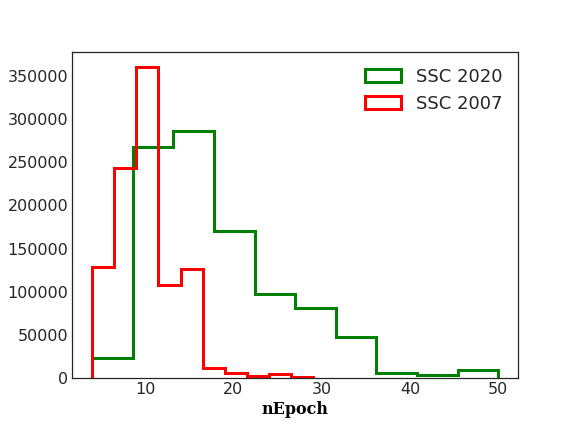
\includegraphics[width=0.4\textwidth, keepaspectratio]{figures/nepoch_compOvsN.png}
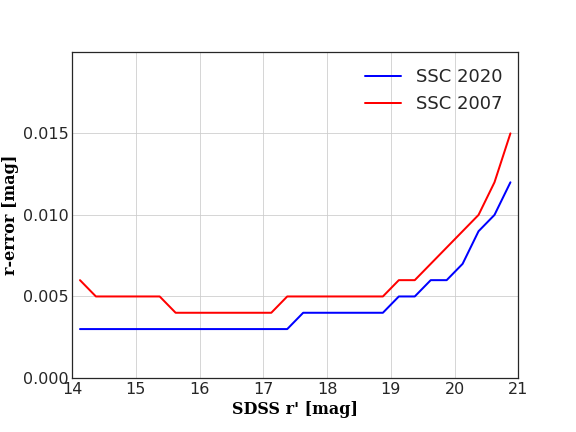
\includegraphics[width=0.4\textwidth, keepaspectratio]{figures/rerr_compOvsN.png}
\caption{{\it Left:} A comparison of the number of observational epochs for matched stars in the 2020 versus 2007 Standard Star Catalog (SSC). {\it Right:} A comparison of the median formal $r$ band photometric uncertainties of matched objects in the 2020 versus 2007 SSC, as a function of their mean $r$ magnitudes.
\label{fig:rerr_nvso}}
\end{figure}


\subsection{The derivation of  photometric zeropoint corrections using Gaia DR2 data\label{sec:GaiaCorr}} 

The variation of photometric zeropoints with position on the sky in the \pOc\ (see their eq.~4) was 
constrained using a combination of stellar colors \citep[the principal axes in color-color diagrams, for details 
see][]{2004AN....325..583I} and a standard star network \citep{2002AJ....123.2121S}. It is likely that 
residual errors in zeropoint calibration (e.g., a saw-tooth pattern, as a function of Declination,
was reported by \citealt{2013A&A...552A.124B}; see their Fig.~23) can be further minimized using 
uniformly calibrated space-based photometry from Gaia Data Release 2 (DR2). 

\subsubsection{Positional matching of the SDSS and Gaia catalogs}
Naively, one would positionally match the SDSS and Gaia DR2 catalogs using a matching radius of 
about 0.3 arcsec because SDSS positions are accurate to better than 0.1 arcsec per coordinate (rms) 
for sources with $r < 20.5$ mag \citep{2003AJ....125.1559P}.  However, observational epochs are
sufficiently different that stellar proper motions need to be accounted for; indeed, we find a very 
strong correlation between the SDSS-Gaia positional differences and proper motions published in 
the Gaia DR2 catalog (see the left panel in  Figure~\ref{fig:GaiaRApm}). After accounting for proper
motions,  the positions agree at the level of $\sim28$ milliarcsec (robust\footnote{We use robust estimator 
of standard deviation computed as $\sigma_G = 0.741*(q_{75}-q_{25})$, where $q_{25}$ and $q_{75}$ are 
the 25\% and 75\% quantiles, and the normalization factor 0.741 assures that $\sigma_G$ is equal to 
standard deviation for normal (Gaussian) distribution.}
rms, per coordinate). The 
residual differences are dominated by systematic errors in SDSS astrometry because there is
no increase of this rms with magnitude (see the right panel in Figure~\ref{fig:GaiaRApm}), and
because the contribution of Gaia's astrometric measurement uncertainties is negligible. 
The implied SDSS astrometric accuracy of $\sim28$ milliarcsec is substantially better than 
``$<0.1$ arcsec reported by \cite{2003AJ....125.1559P}, but note that here we used 
positions ``averaged'' over typically $\sim20$ SDSS runs (see the left panel in Figure~\ref{fig:rerr_nvso}). 

\begin{figure}[t]
\centering 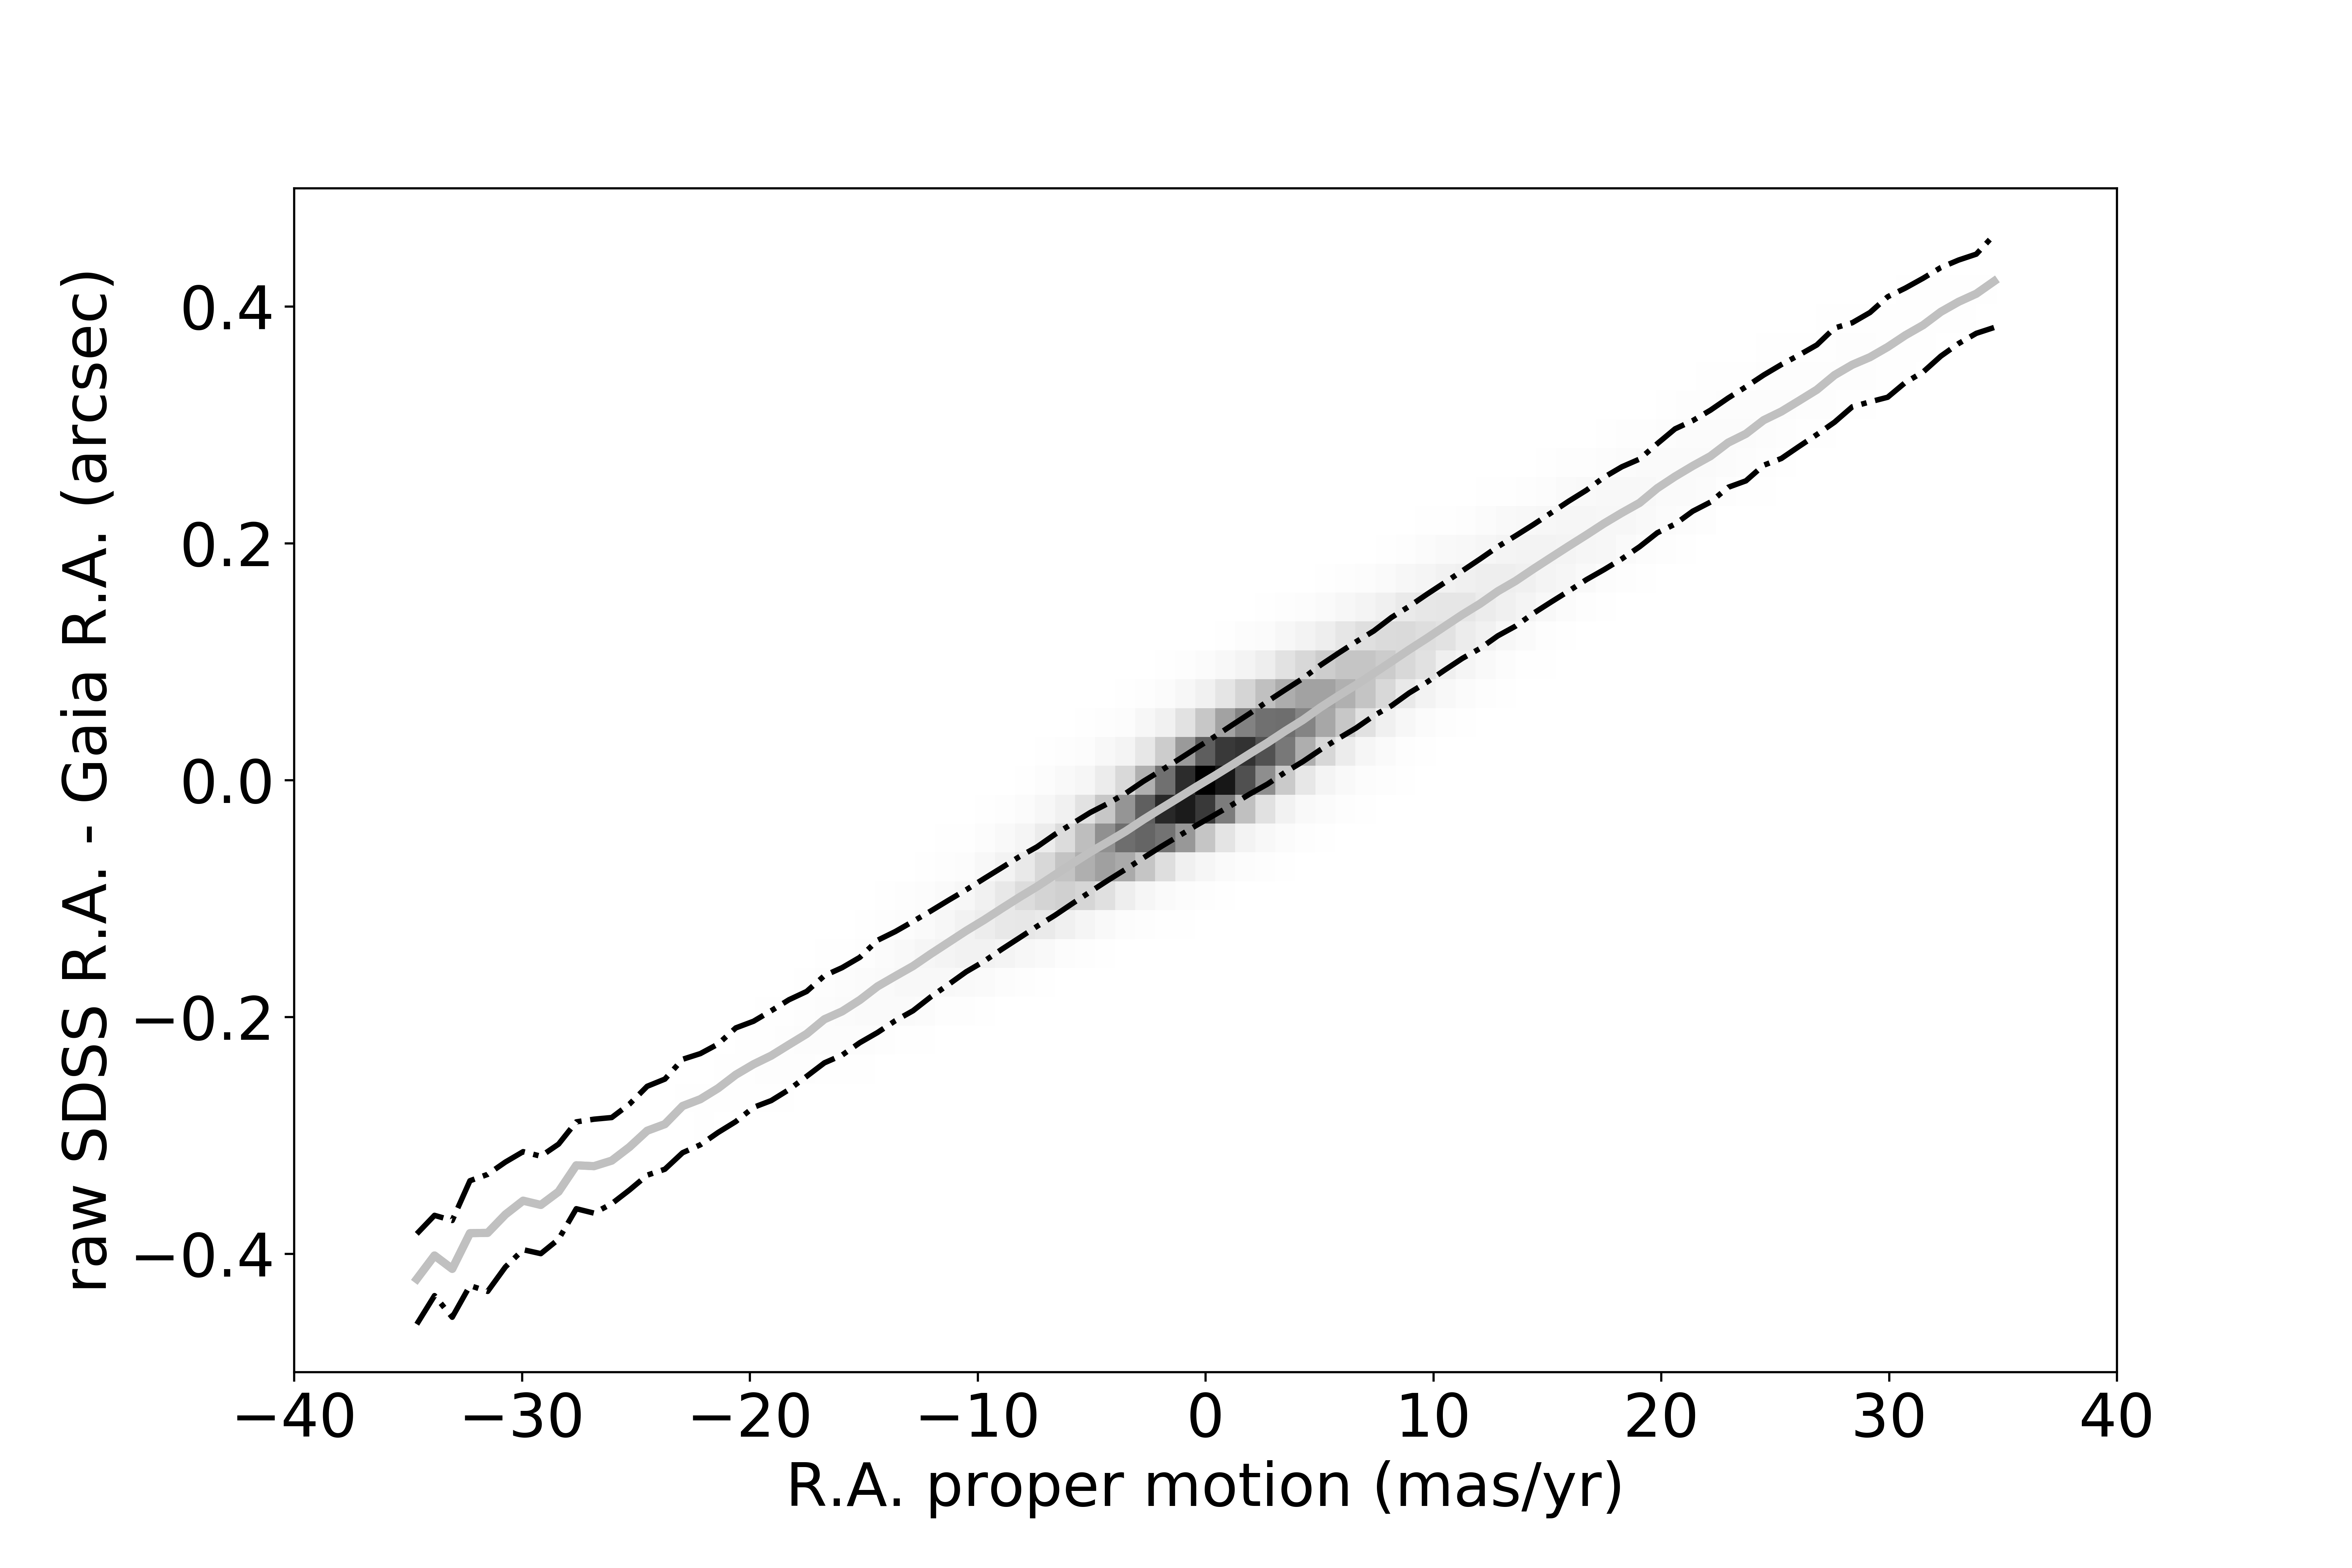
\includegraphics[width=0.4\textwidth, keepaspectratio]{figures/astroVSpm_RA_pm.png}
\centering 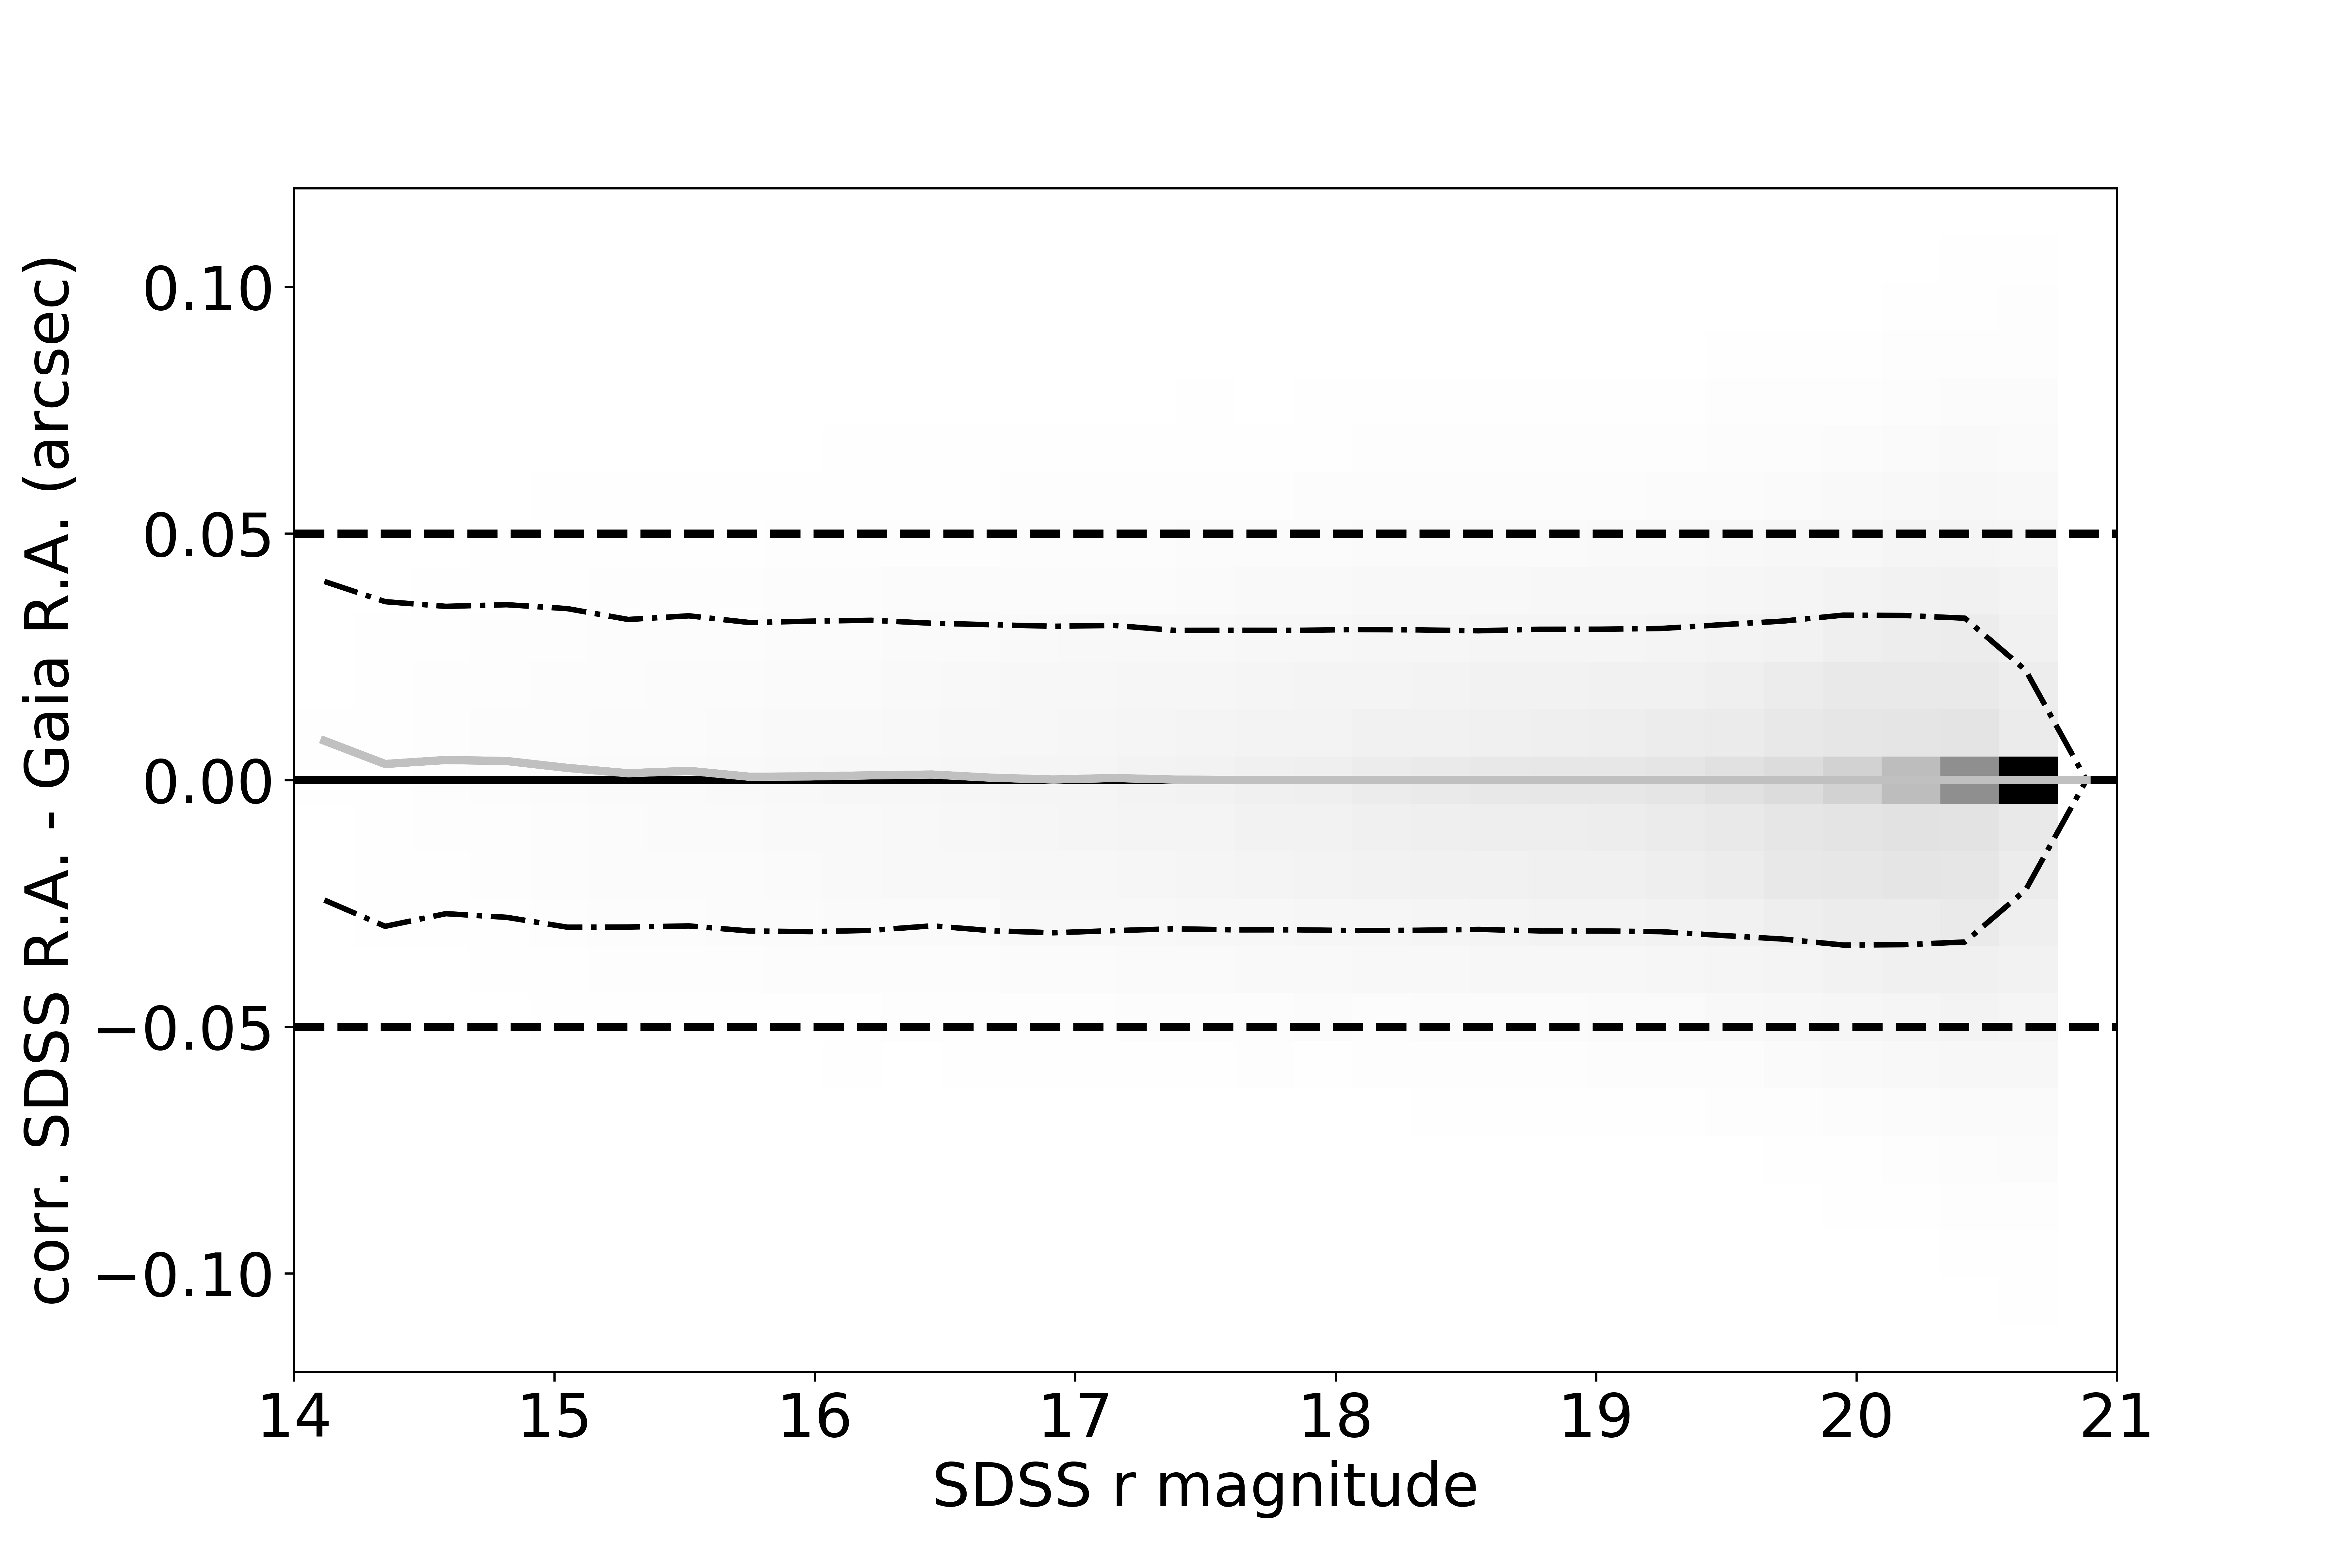
\includegraphics[width=0.4\textwidth, keepaspectratio]{figures/astroVSpm_RA_r.png}

\caption{The left panel shows the R.A. difference between SDSS and Gaia 
vs. R.A. proper motion reported by Gaia DR2. The solid line shows the median difference in bins 
of proper motion and the dashed lines mark the $\pm \sigma_G$ envelope around the medians,
where $\sigma_G$ is the robust standard deviation. The right panel shows the R.A. difference 
after correcting using the best-fit R.A. difference vs. 
proper motion curve, as a function of the SDSS $r$ magnitude. As evident, the residual differences are dominated 
by systematic errors in SDSS astrometry at the level of $\sim28$ milliarcsec (note that there is no increase with 
magnitude). Analogous plots for Declination quantities are similar. 
\label{fig:GaiaRApm}}
\end{figure}
  

\subsubsection{Gaia-based photometric zeropoint corrections}

Gaia DR2 reported Gmag magnitudes, which approximately span the SDSS $griz$ bandpasses, 
and BP and RP magnitudes, which approximately correspond to the blue and red halfs of the 
Gmag bandpass. We first used Gmag data to derive ``gray'' zeropoint corrections (applied to
all five SDSS bands), and then use the BP-RP color to derive zeropoint corrections for the 
$ugiz$ bands, relative to the $r$ band. 

The basic idea is simple: use Gaia's Gmag, Gmag$_{GaiaDR2}$, and the SDSS $gri$ magnitudes
to derive synthetic Gmag magnitudes based on SDSS data, Gmag$_{SDSS}$; bin the 
$\Delta$Gmag = (Gmag$_{SDSS}$-Gmag$_{GaiaDR2}$) residuals by R.A. and Dec, and 
use the median residuals per bin as the gray correction for SDSS photometry (as functions
of R.A. and Dec). Similarly, use Gaia's BP-RP color to derive synthetic $u-r$, $g-r$, $r-i$
and $r-z$ colors, and used the median residuals per bin as zeropoint corrections for 
the $ugiz$ bands. 

Given a large number of matched stars ($\sim 400,000$), and a large number of color combinations,
we do not attempt to derive analytic fits for synethtic magnitudes and colors but instead
use 0.05 mag narrow color bins and linear interpolation between the bins. We have verified
that even sixth-order polynomial fits do not provide better results than this simple 
numerical approach. An example of such a transformation is shown in Figure~\ref{fig:GrVSgi}. 

The variation of Gmag residuals shows two interesting features. First, there is a sharp
``jump'' by about 3 millimag at Gmag$\sim$16.  This jump was a known (and 
larger problem) in Gaia Data Release 1, but appears not entirely fixed in DR2. The 
second ``feature'' is a large ($\sim0.01-0.02$ mag) discrepancy at the faint end:
about $\sim$10 millimag at Gmag=19.5 and $\sim$20 millimag at Gmag=20.5. 
A comparison of the SDSS catalog with Pan-STARRS and DES catalogs (see 
Section~\ref{sec:DESPS1} and Figure~\ref{fig:drVSr}) strongly suggests that the
origin of this discrepancy is a bias in Gaia's Gmag photometry at the faint end, rather 
than a problem with SDSS catalog (offsets between the SDSS and DES
photometry are $<1-2$ millimag at Gmag$\sim$20.5). 
 
Given these two features, we limit the calibration sample to the $16<$Gmag$<19.5$
magnitude range. We further restrict calibration stars to the $0.4 < g-i < 3.0$ color 
range (approximately A0 to M5 spectral range), yielding a sample of $\sim372,000$ stars. 
The behavior of median Gmag residuals per R.A. and Declination bin is shown in 
Figures~\ref{fig:graycorrRA} and \ref{fig:graycorrDec}. 

Except for a few degrees long region at the edge of Stripe 82 (R.A.$>$55 deg), the
SDSS photometric zeropoints are remarkably stable with respect to R.A.; the scatter
is only 3.5 millimag. On the other hand, there are clear deviations in Declination 
direction, which clearly map to the 12 scanning strips that fill Stripe 82. We note
that discrepancies never exceed 0.01 mag (with a scatter of 6.2 millimag), which was 
the claimed accuracy of the \pOc. Thanks to a large number of stars in the sample,
and well calibrated Gaia's photometric zeropoints across the sky, we can now 
constrain SDSS zeropoints with a precision of about 1 millimag per 0.01 degree
wide Declination bin. 

The residuals shown in Figures~\ref{fig:graycorrRA} and \ref{fig:graycorrDec} are
applied as ``gray'' zeropoint corrections to $ugriz$ magnitudes, as functions of 
R.A. and Declination, to all 991,472 stars in the catalog. This catalog version was
labeled v3.1, and it is publicly available\footnote{See http://faculty.washington.edu/ivezic/sdss/catalogs/stripe82.html}. 

In the next re-calibration step, we derive synthetic $u-r$, $g-r$, $r-i$ and $r-z$ colors
from Gaia's BP-RP color, using the same binning procedure as we used above for 
Gmag$-r$ vs. $g-i$ variation (see Figure~\ref{fig:GrVSgi}). An example of color residuals 
is shown in Figure~\ref{fig:riresid}.  The median residuals per R.A. and Declination bins 
are then used as zeropoint corrections for the $ugiz$ bands. The robust standard deviation 
for all zeropoint corrections is listed in Table~\ref{tab:GaiaRMS}. 

The largest corrections were derived for the $u$ band. Given that Gaia's BP-RP
color does not strongly constrain the $u$ band flux, we used the CFIS catalog 
(see Section~\ref{ssec:cfis}) as an independent verification test. We verified that
zeropoint errors in the SDSS catalog implied by Gaia's and CFIS data agree in
Declination direction, but found inconsistencies for R.A. bins. For this reason,
we only applied $u$ band correction in Declination direction. The plausible 
$u$ band zeropoint errors in the new catalog are further discussed in Section~\ref{sec:CFIStest}. 
This final catalog version was labeled v3.4, and it is also publicly available. 



\begin{deluxetable}{l|c|c}[ht!]
\tablecaption{The robust standard deviation for binned SDSS-based vs. Gaia-based color residuals$^a$. \label{tab:GaiaRMS}}
\tablehead{
\colhead{Color } & \colhead{rms for R.A.} & \colhead{rms for Dec}
}
\startdata
 gray (Gmag) &    3.5         &    6.2   \\
    $u-r$        &   0.0$^b$  &   20.4   \\     
    $g-r$        &   4.0         &    4.2    \\
    $r-i$         &   4.1         &    3.2    \\ 
    $r-z$        &   7.4         &    2.9    \\ 
\enddata
\tablenotetext{a}{The robust standard deviation is estimated using interquartile range. The units are millimag.} 
\tablenotetext{b}{For the $u$ band, we could not confirm the R.A. behavior of Gaia-based zeropoint correction 
with the CFIS data and didn't apply it. The large $u$ band correction as a function of Declination was validated 
with the CFIS data (see Section~\ref{sec:CFIStest}).} 
\end{deluxetable}
  


\begin{figure}
  \centering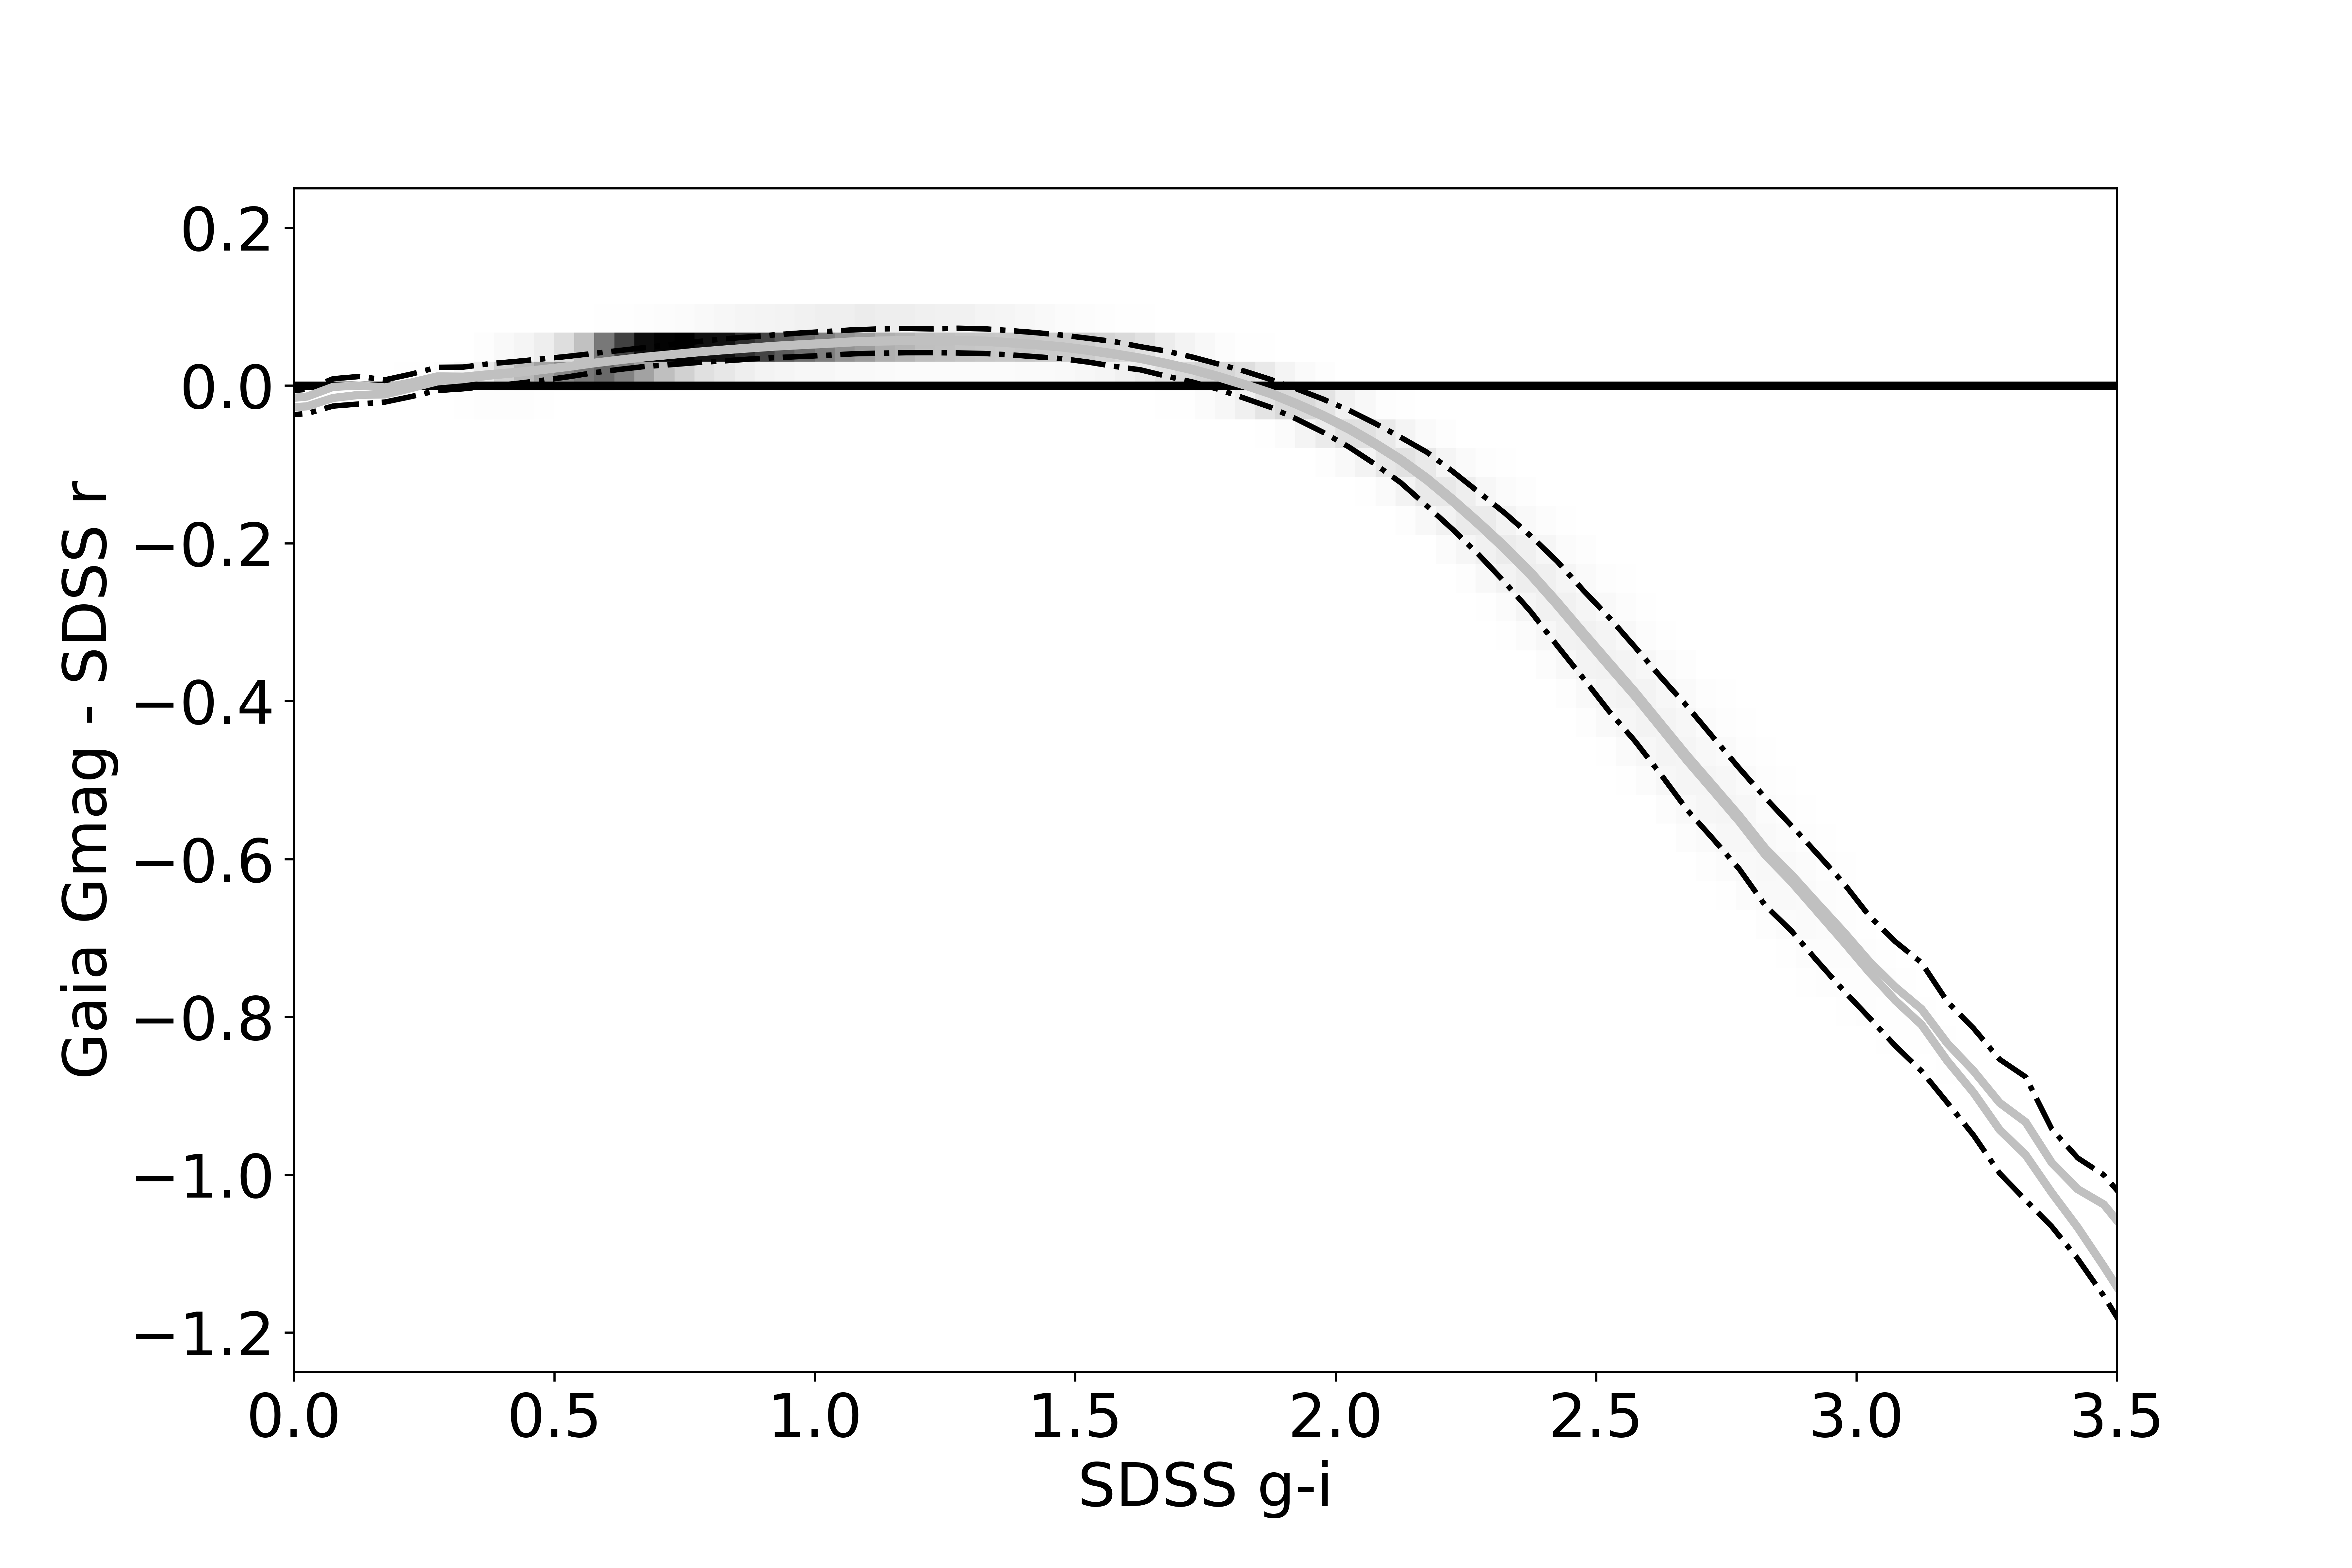
\includegraphics[width=8cm]{figures/GrVSgi.png} 
\caption{The variation of the difference between Gaia's Gmag magnitude from Data Release 2
and SDSS $r$ magnitude with the SDSS $g-i$ color.
The  color map illustrates the distribution of $\sim 393,000$ matched stars with 
$16<$Gmag$<19.5$. The two (barely distinguishable) solid lines represent the median 
values $\pm$ uncertainty of the median for 0.05 mag wide $g-i$ bins. The short-dashed 
lines show the median values $\pm$ the robust standard deviation for 
each bin. The horizontal solid line at zero is added to guide the eye. The mean of 
the two solid lines is used to derive the gray zeropoint correction, as a function of R.A.
and Declination.}
\label{fig:GrVSgi}
\end{figure}


\begin{figure}
    \centering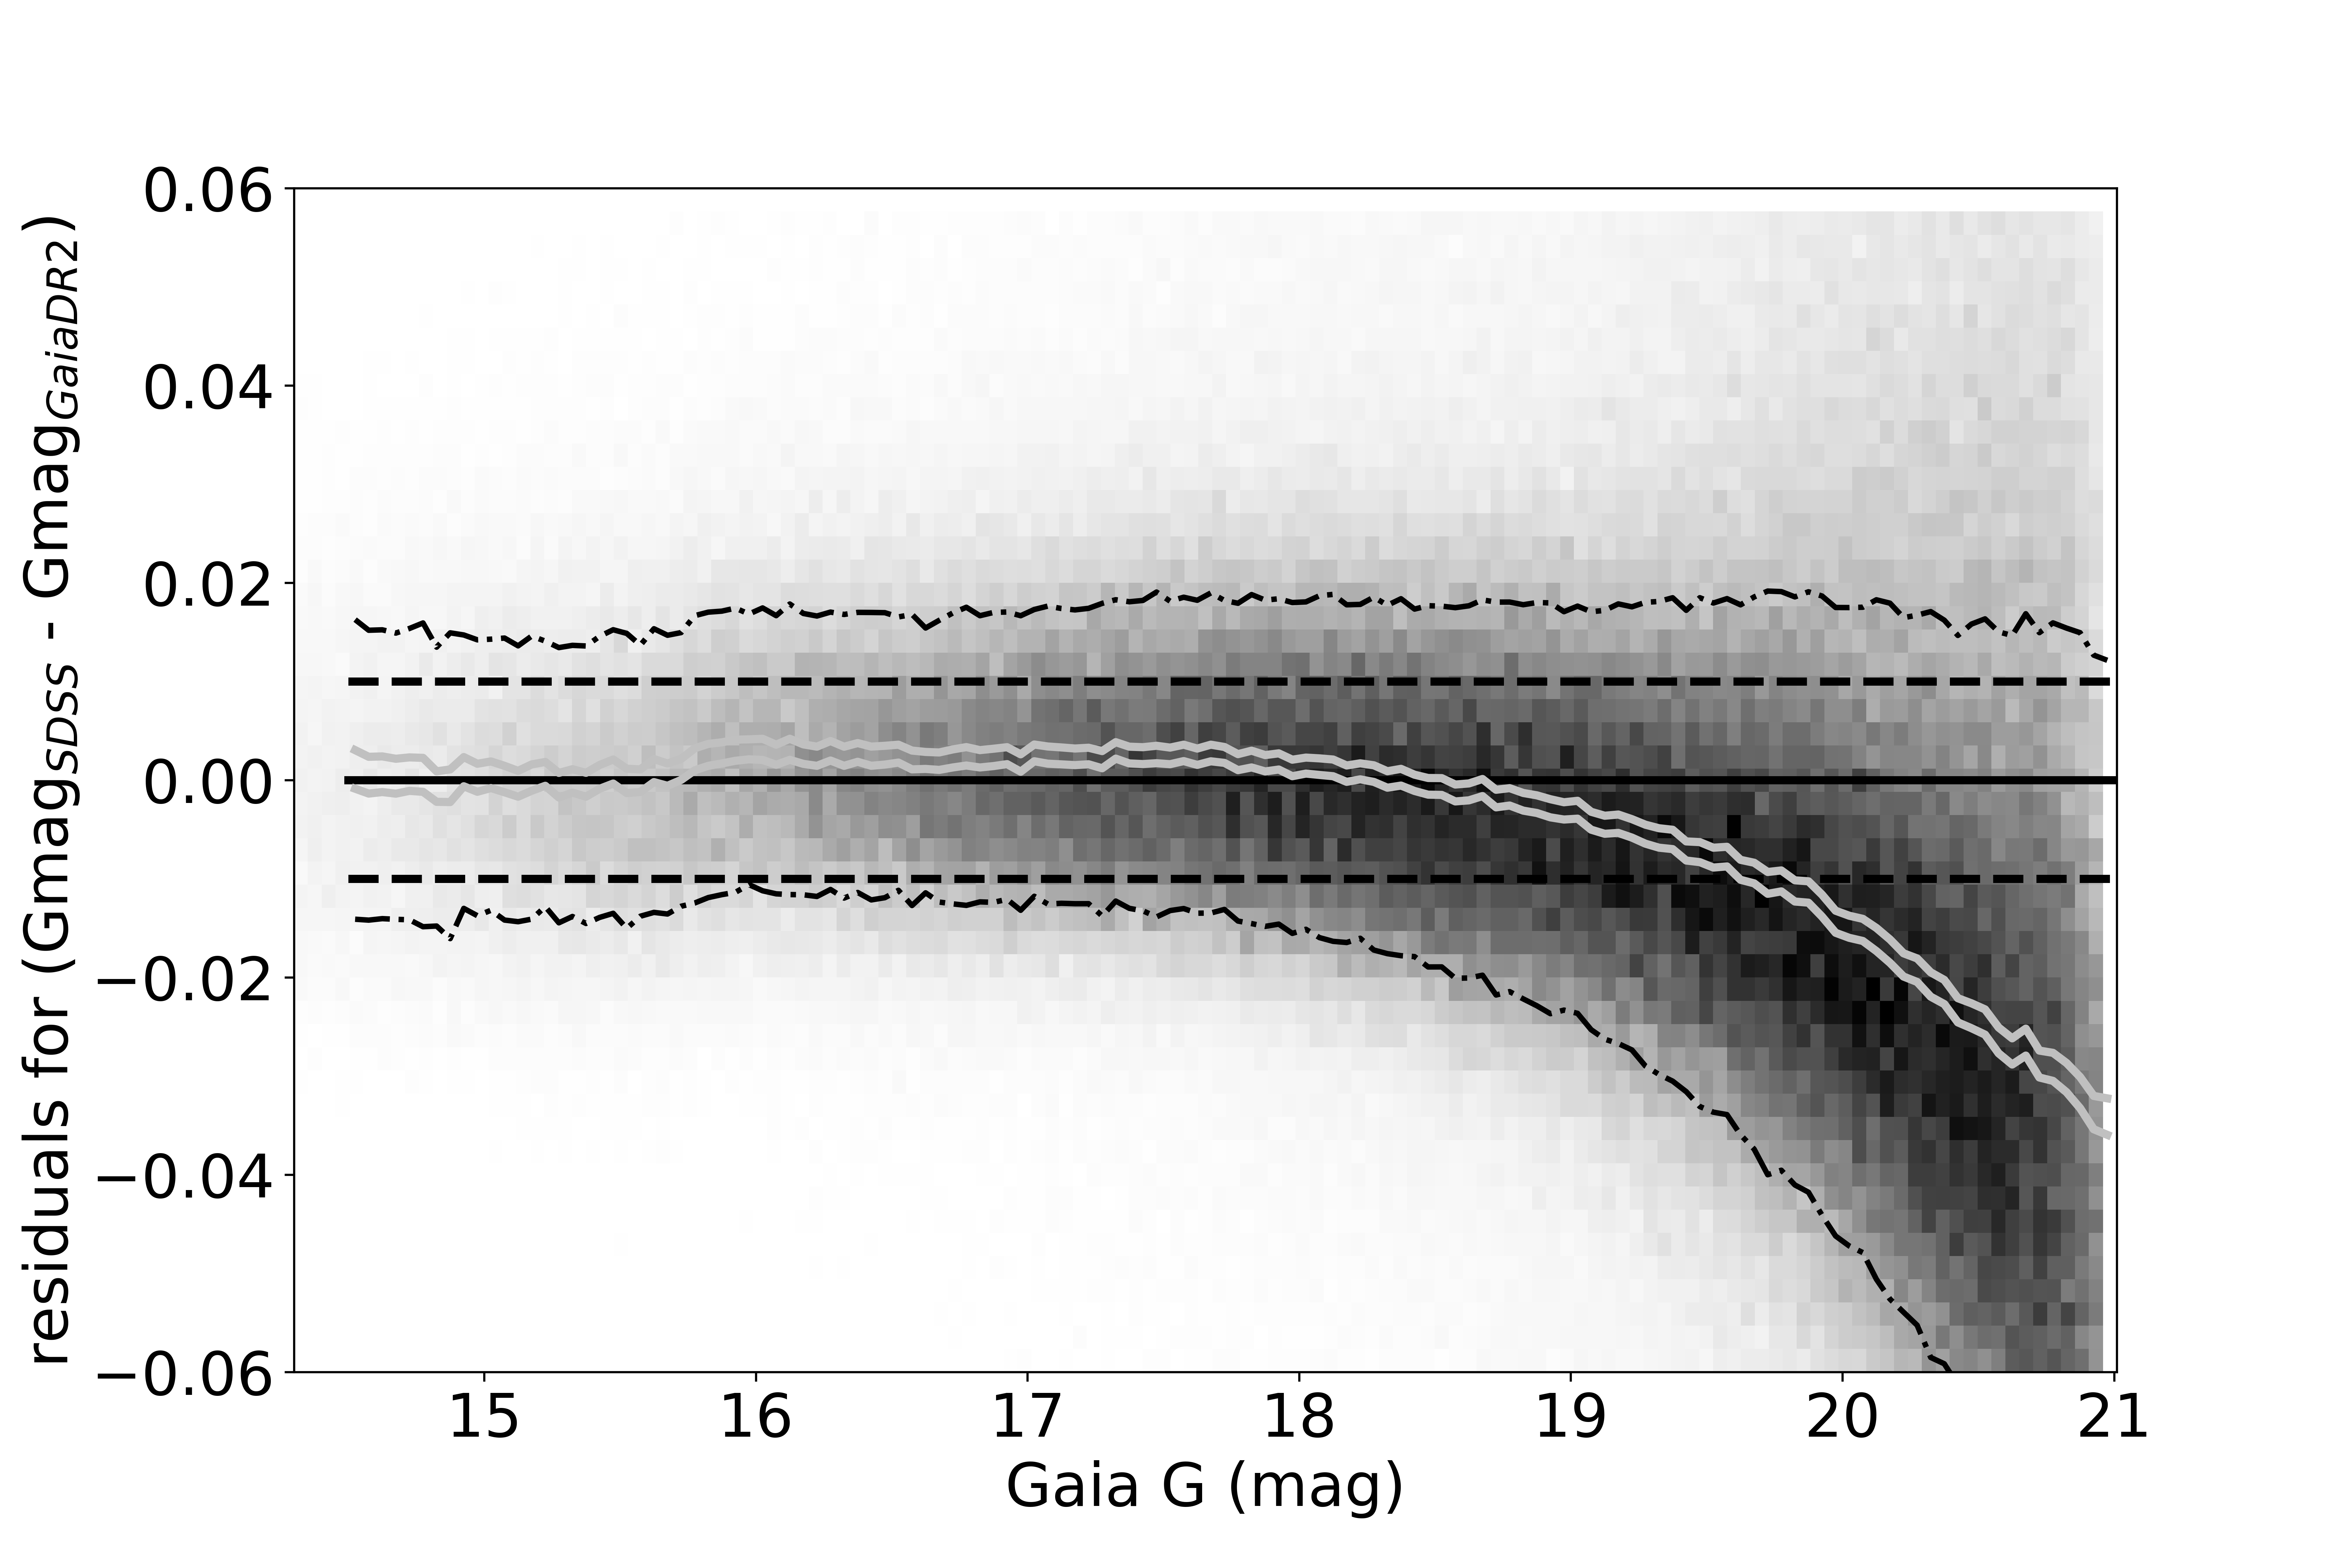
\includegraphics[width=9cm]{figures/GmagCorrectionTest_Gmag_Hess.png} 
\caption{The variation of the residuals between Gaia's Gmag from Data Release 2
and synthetic Gmag values generated using SDSS $gri$ photometry. The two solid 
lines represent the median values $\pm$ uncertainty of the median for each
0.05 mag wide Gmag bin. The short-dashed lines show the median values $\pm$ 
the robust standard deviation for each bin. The horizontal solid and long-dashed 
lines at zero and $\pm$0.01 mag, respectively, are added to guide the eye.
Note the jump by about 3 millimag at Gmag$\sim$16 -- this jump was a known and 
larger problem in Gaia Data Release 1, and apparently not entirely fixed in DR2. 
Note also large ($\sim0.01-0.02$ mag) discrepancy at the faint end -- a comparison 
of the SDSS catalog with Pan-STARRS and DES catalogs (see Figure~\ref{fig:drVSr}) 
suggests that its origin is a bias in Gaia's photometry at the faint end, rather than 
a problem with SDSS photometry.}
\label{fig:gaiaJump}
\end{figure}


\begin{figure}
  \centering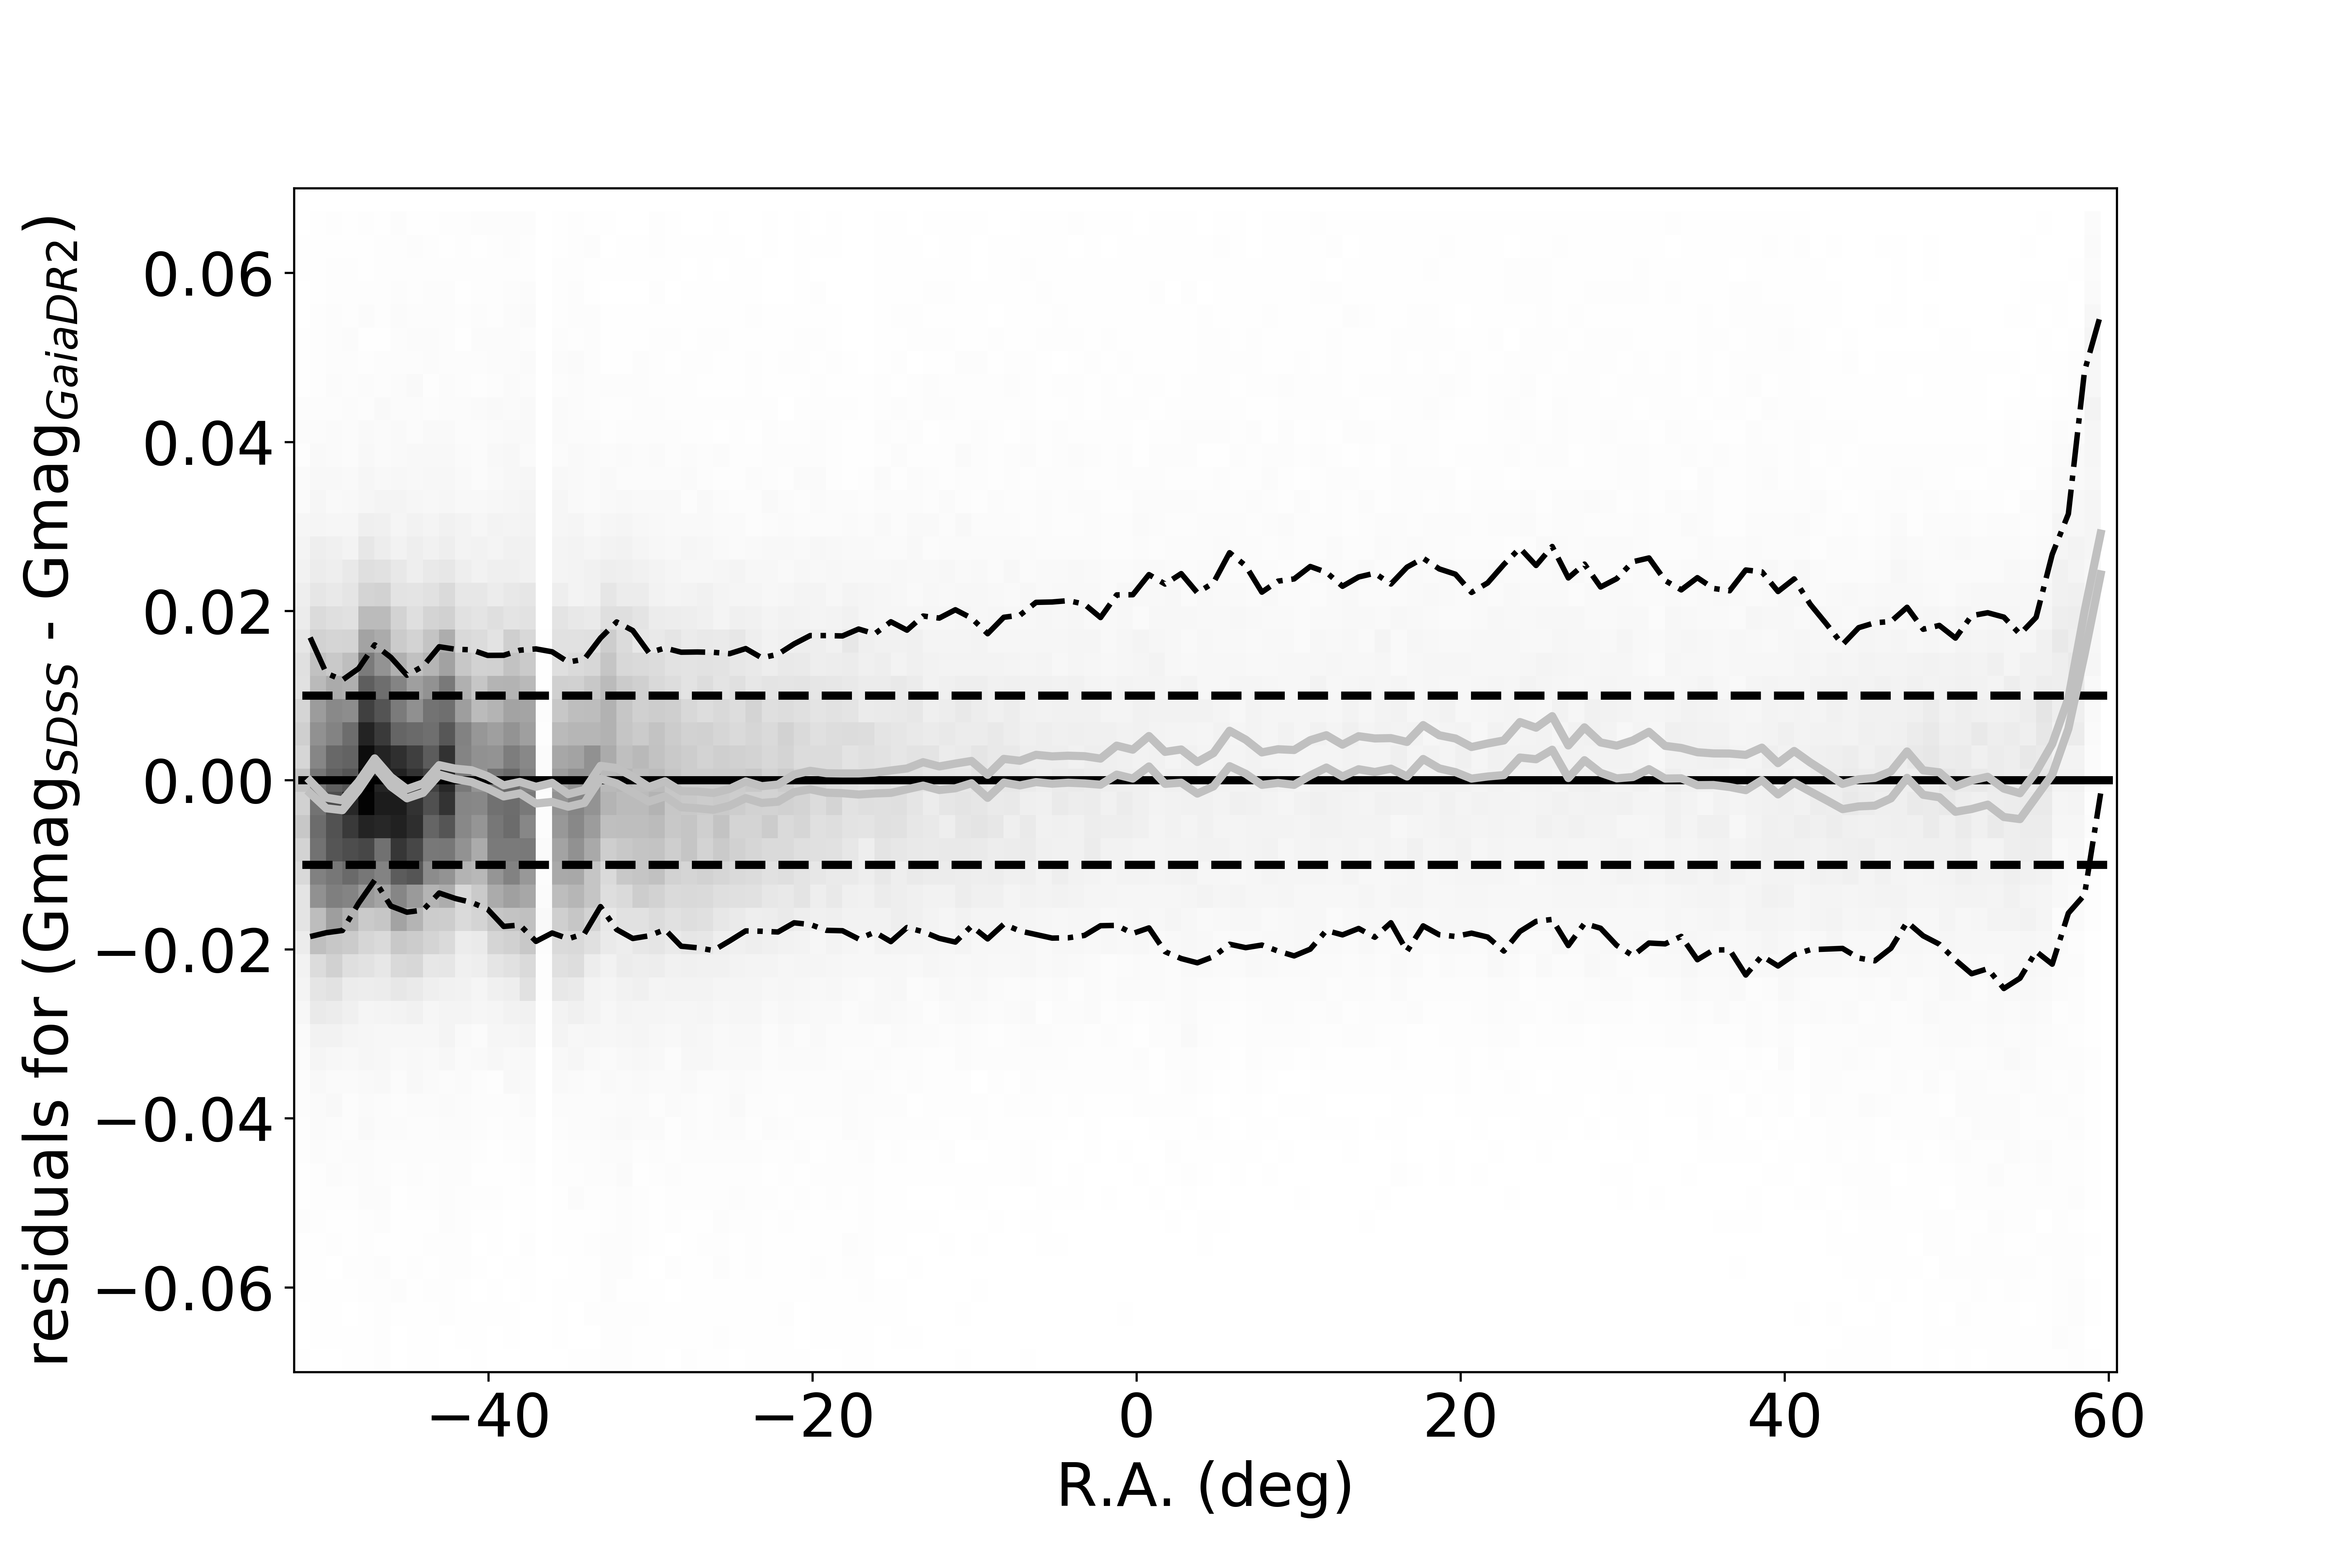
\includegraphics[width=8cm]{figures/GmagCorrection_RA_Hess.png} 
\caption{The R.A. variation of the residuals between Gaia's Gmag from DR2
and synthetic Gmag values generated using SDSS $gri$ photometry. The 
color map illustrates the distribution of $\sim 372,000$ matched stars with 
$16<$Gmag$<19.5$ and $0.4 < g-i < 3.0$. The two solid lines represent the 
median values $\pm$ uncertainty of the median for 1 degree wide R.A. bins. 
The short-dashed lines show the median values $\pm$ the robust standard 
deviation for each bin. The horizontal solid and long-dashed lines at zero and 
$\pm$0.01 mag, respectively, are added to guide the eye. The mean of the two 
solid lines is the gray correction, as a function of R.A., applied to the SDSS 
$ugriz$ magnitudes. The standard deviation for the applied correction is 3.5 millimag.}
\label{fig:graycorrRA}
\end{figure}

\begin{figure}
    \centering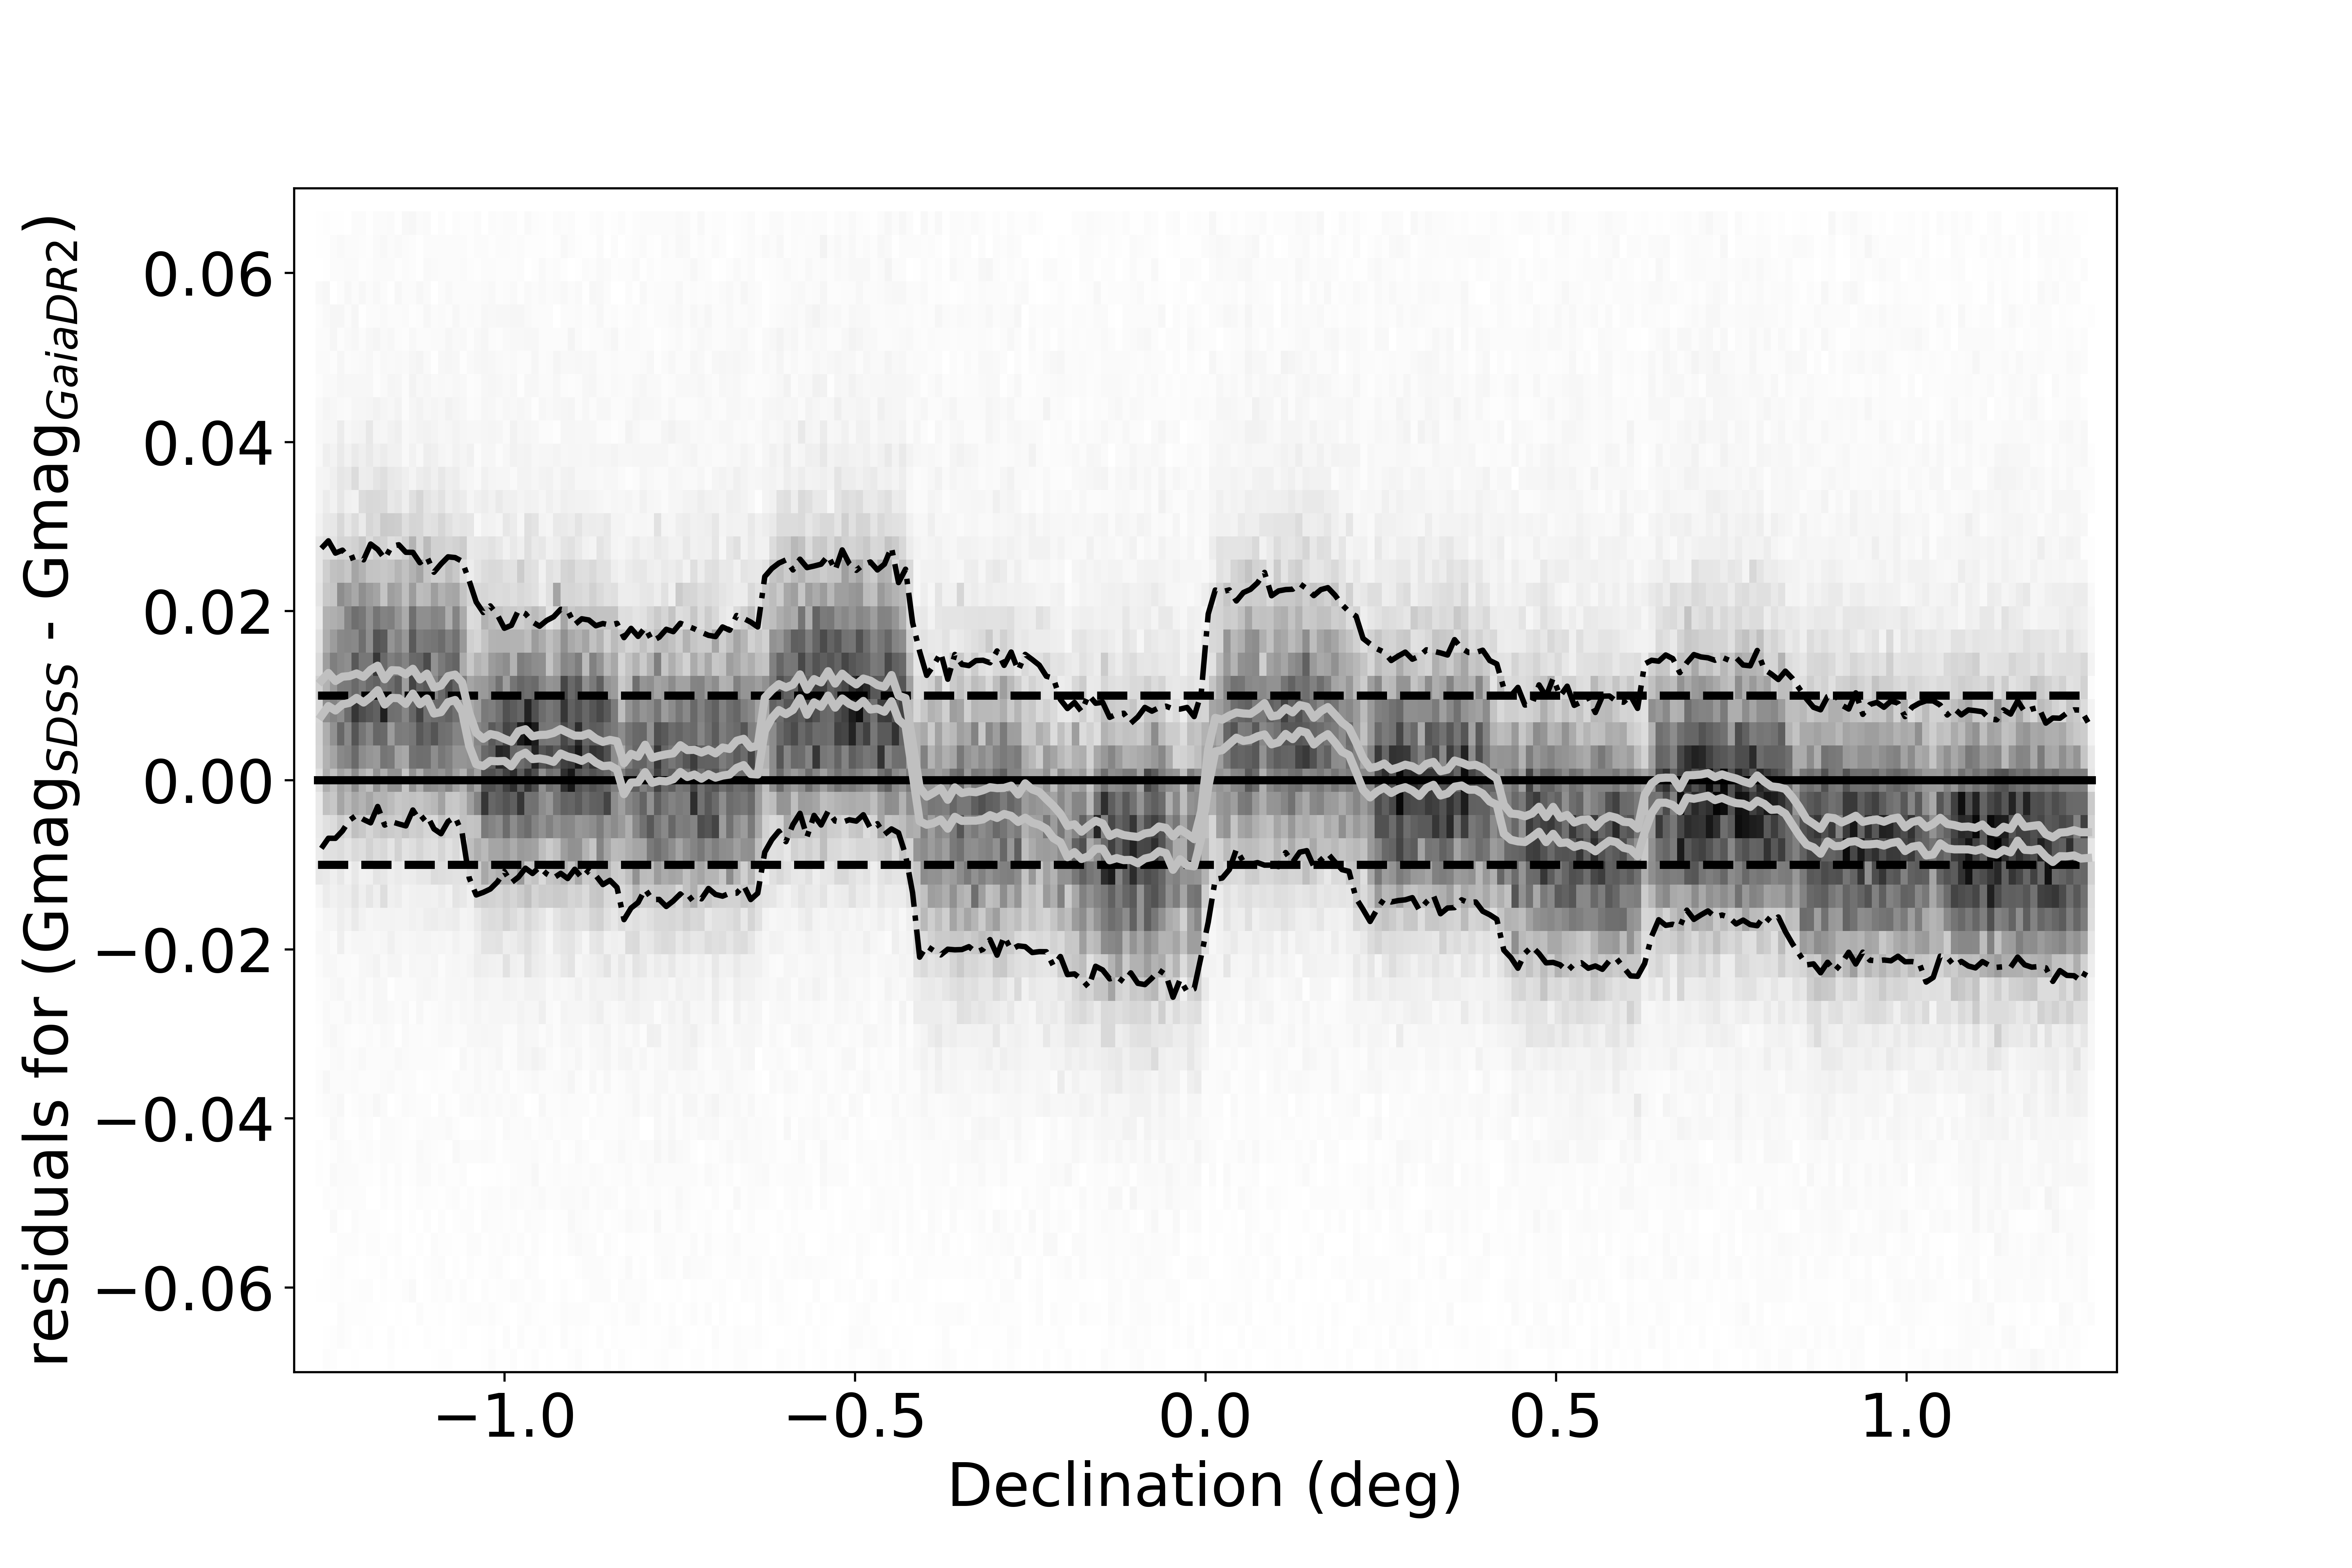
\includegraphics[width=9cm]{figures/GmagCorrection_Dec_Hess.png} 
\caption{Analogous to Figure~\ref{fig:graycorrRA}, except that here results are shown for
0.01 degree wide Declination bins. The 12 cleary visible regions correspond to
two SDSS scans (in R.A. direction) and six CCD columns in the SDSS camera. 
The standard deviation for the applied correction is 6.2 millimag, with a maximum
absolute value of $\sim0.01$ mag.}
\label{fig:graycorrDec}
\end{figure}



\begin{figure}
    \centering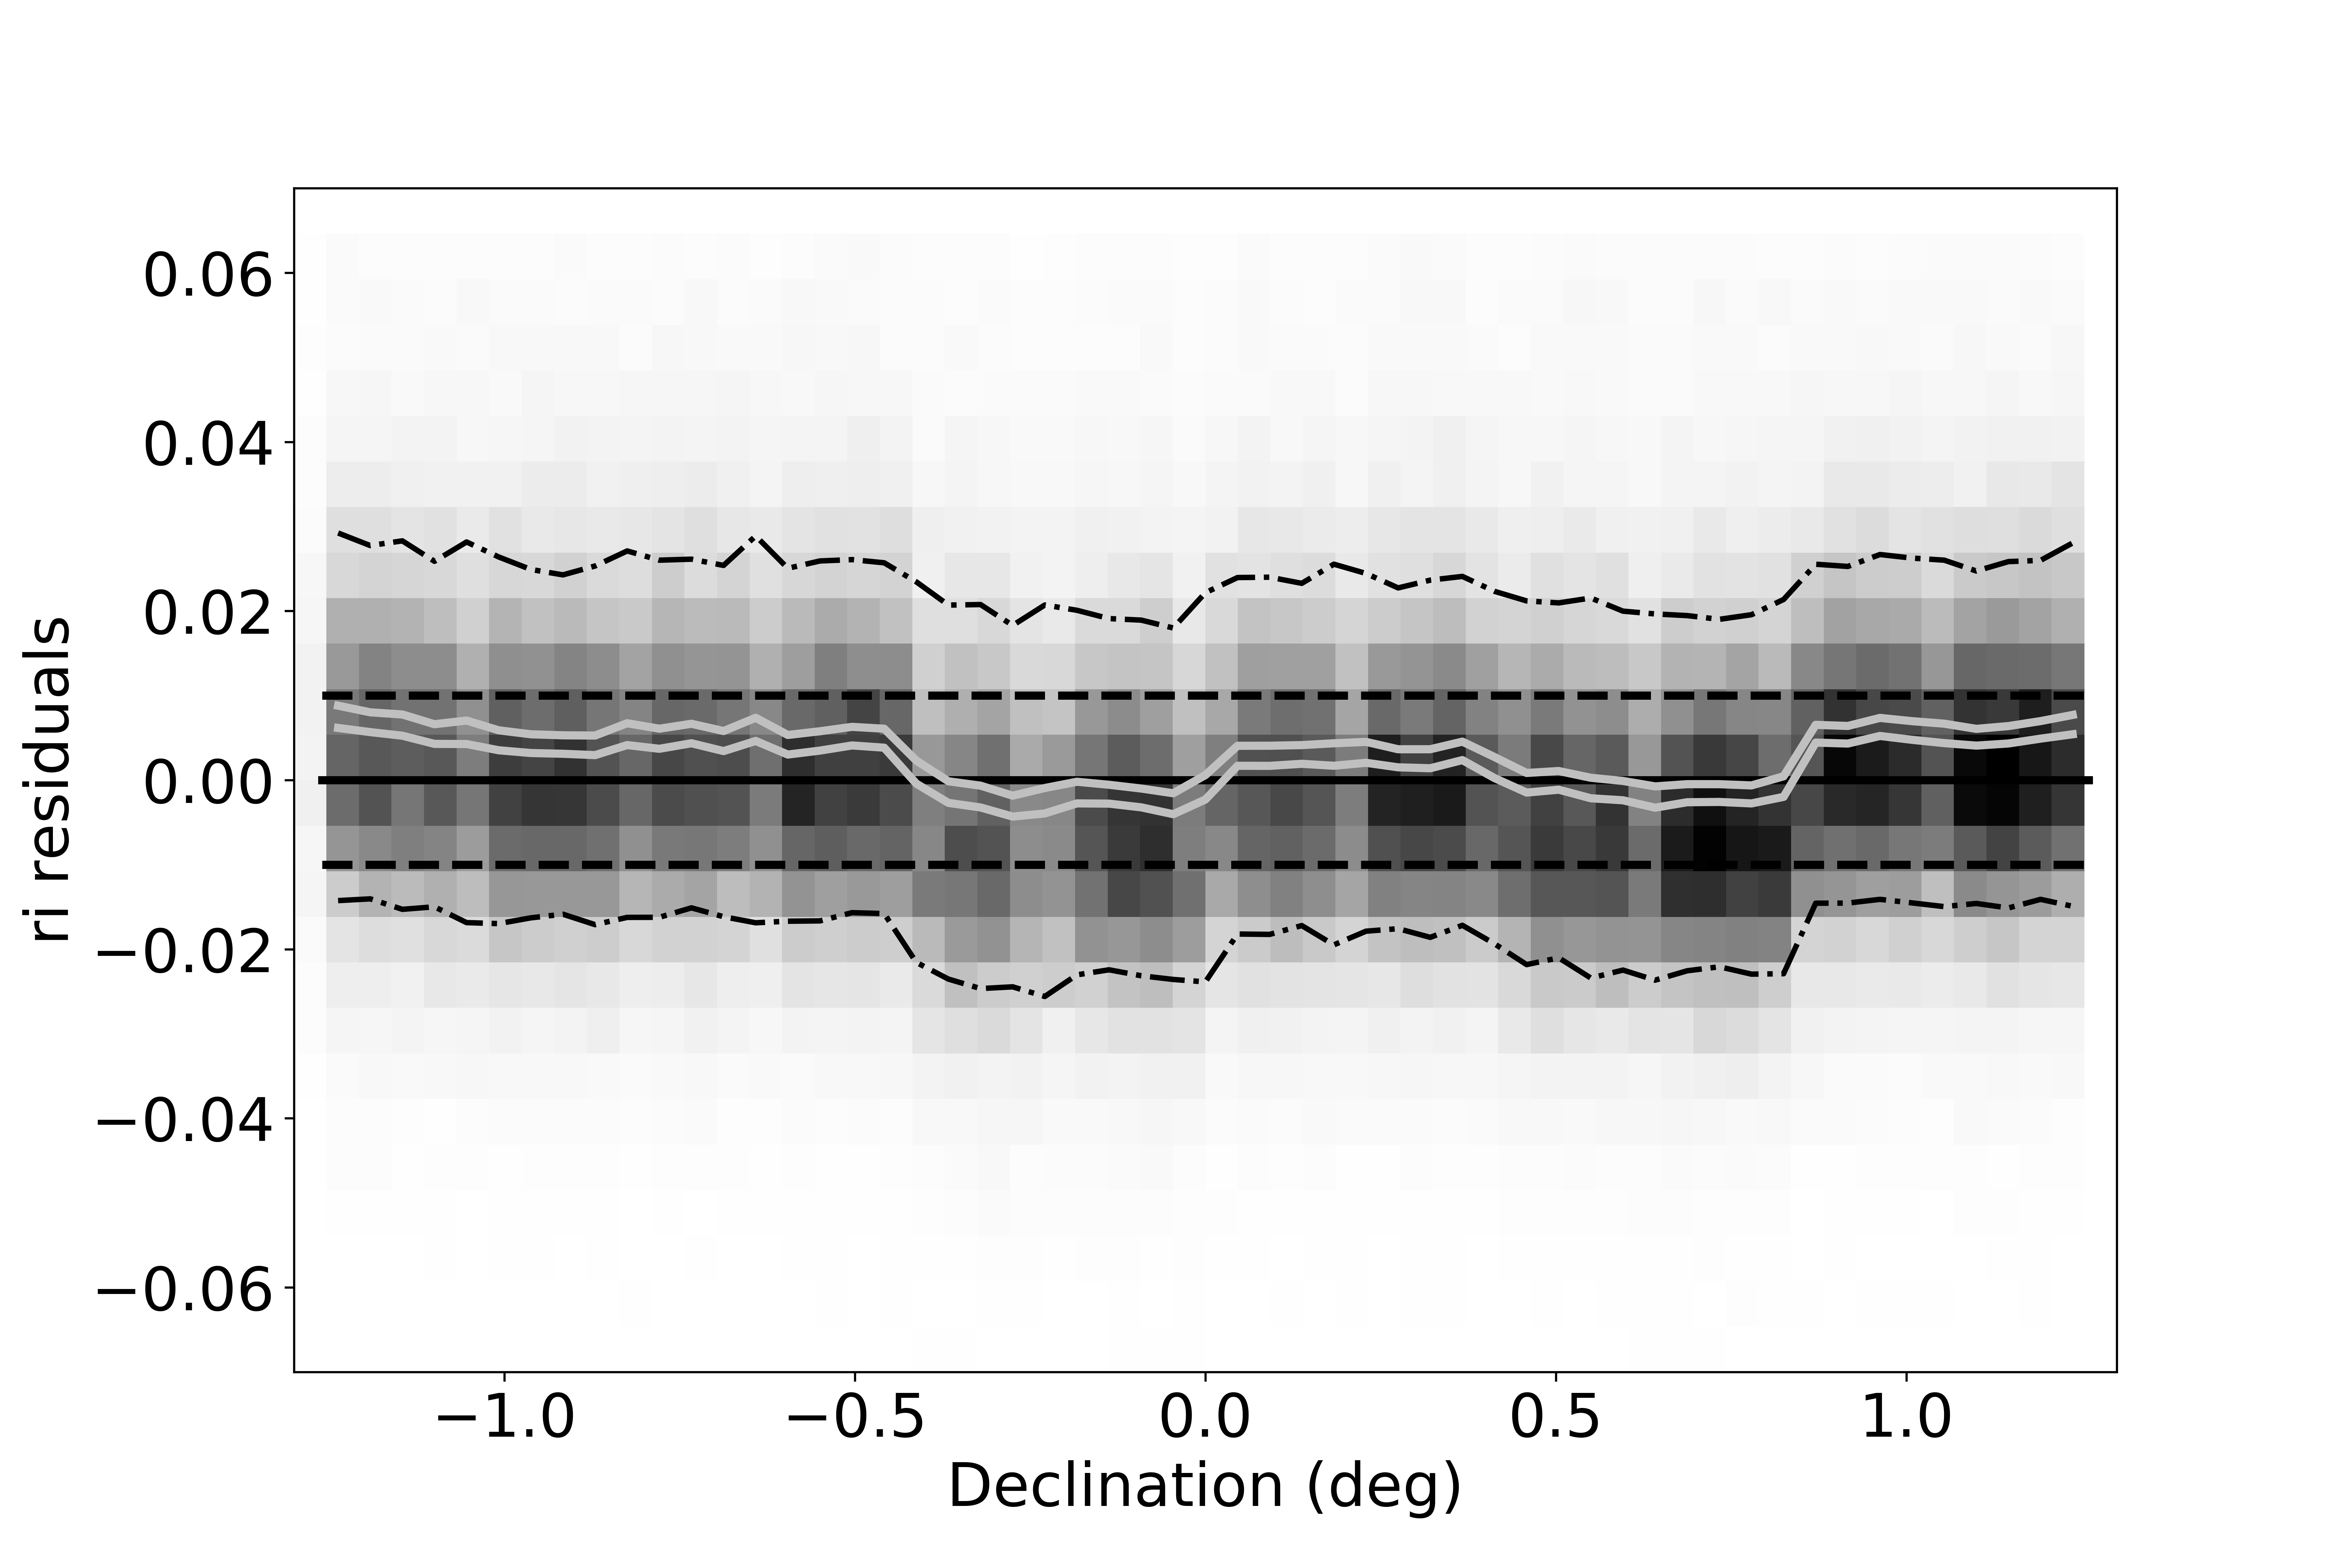
\includegraphics[width=9cm]{figures/colorResidGaiaColorsB_ri_Dec_Hess.png} 
\caption{Analogous to Figure~\ref{fig:graycorrDec}, except that here residuals 
correspond to differences between the SDSS $r-i$ color and a synthetic $r-i$ color
generated using Gaia's $BP-RP$ color. Note the signature of SDSS camera columns
at the level of a few millimags. The standard deviation for the binned medians is 
3.2 millimag (for other bands, please see Table~\ref{tab:GaiaRMS}.}
\label{fig:riresid}
\end{figure}





\subsection{Comparison of the SDSS v2.6 and v3.4 catalogs \label{sec:v26v34}} 
 
The v2.6 (``old'') SDSS Standard Star Catalog has been extensively used 
\citep[e.g.,][]{2008AJ....135..338F},
and here we briefly analyze differences between the v3.4 (``new'') and v2.6 magnitudes
to inform the future users about catalog consistency. 
In our analysis, we first compare v2.6 and v3.4 magnitudes of individual stars and 
bin the differences by R.A., Declination and magnitude. 

On average, both catalog versions are on the same magnitude scale (the median $ugriz$ 
magnitude differences for all stars are zero by construction). There are no systematic offsets 
when binned by magnitude, as illustrated in Figure~\ref{fig:v26v34drDec}. The most obvious 
differences appear when magnitude differences are binned by Declination. An example is 
shown in Figure~\ref{fig:v26v34drDec}, where the periodicity of residuals corresponds to the 
field-of-view size for the SDSS Photometric Calibration Telescope \citep{2002AJ....123.2121S}. 
The standard deviation for median values per bin is 6.8 millimag, with extreme values about 
0.01 mag. It is likely that systematic errors in the calibration star network photometry 
were propagated through ``flat-field corrections'' discussed by \pO\ to the v2.6 catalog.
We note that these errors, now found thanks to Gaia catalogs, are well within the claimed
photemetric accuracy by both \pO\ and \cite{2002AJ....123.2121S}. 

Given the quality of Gaia photometry, there should be no doubt that SDSS $ugriz$ photometry
reported in the new v.3.4 catalog is superior to the old v2.6 catalog. Nevertheless, we perform
additional tests, based on the position of the stellar locus in the $g-r$ vs. $u-g$, $r-i$ vs. $g-r$ 
and $i-z$ vs. $r-i$ color-color diagrams  \citep{2004AN....325..583I}. The tests are based
on the second principal color for the blue part of the stellar locus, whose median should 
not deviate from zero by construction. Figure~\ref{fig:comparew} compares the behavior
of the $w$ color for the old v2.6 and new v3.4 catalog and demonstrates that the $gri$
photometry is better calibrated in the latter. The behavior of the $s$ and $y$ colors for the 
new catalog is shown in Figure~\ref{fig:comparesy}. Based on these tests, we find that 
the contribution of the zeropoint errors is $<5$ millimag to $gri$ photometry, and 
$<10$ millimag for the $u$ and $z$ bands. 


\begin{deluxetable}{l|c|c}[ht!]
\tablecaption{The robust standard deviation for magnitude differences between the v2.6 (old)
and v3.4 (new) catalogs. \label{tab:oldnewRMS}}
\tablehead{
\colhead{Band} & \colhead{rms for R.A.} & \colhead{rms for Dec}
}
\startdata
       $u$        &        2.3$^a$    &    25.5      \\
       $g$        &        4.5    &      9.4      \\  
       $r$         &        2.0    &      7.0      \\  
       $i$         &        5.3    &      6.5      \\ 
       $z$        &        8.9    &      8.4      \\ 
\enddata
\tablenotetext{a}{For the $u$ band, the scatter in R.A. direction is due to more observations
in v3.4 than in v2.6, rather than zeropoint correction.} 
\end{deluxetable}
   

\begin{figure}
    \centering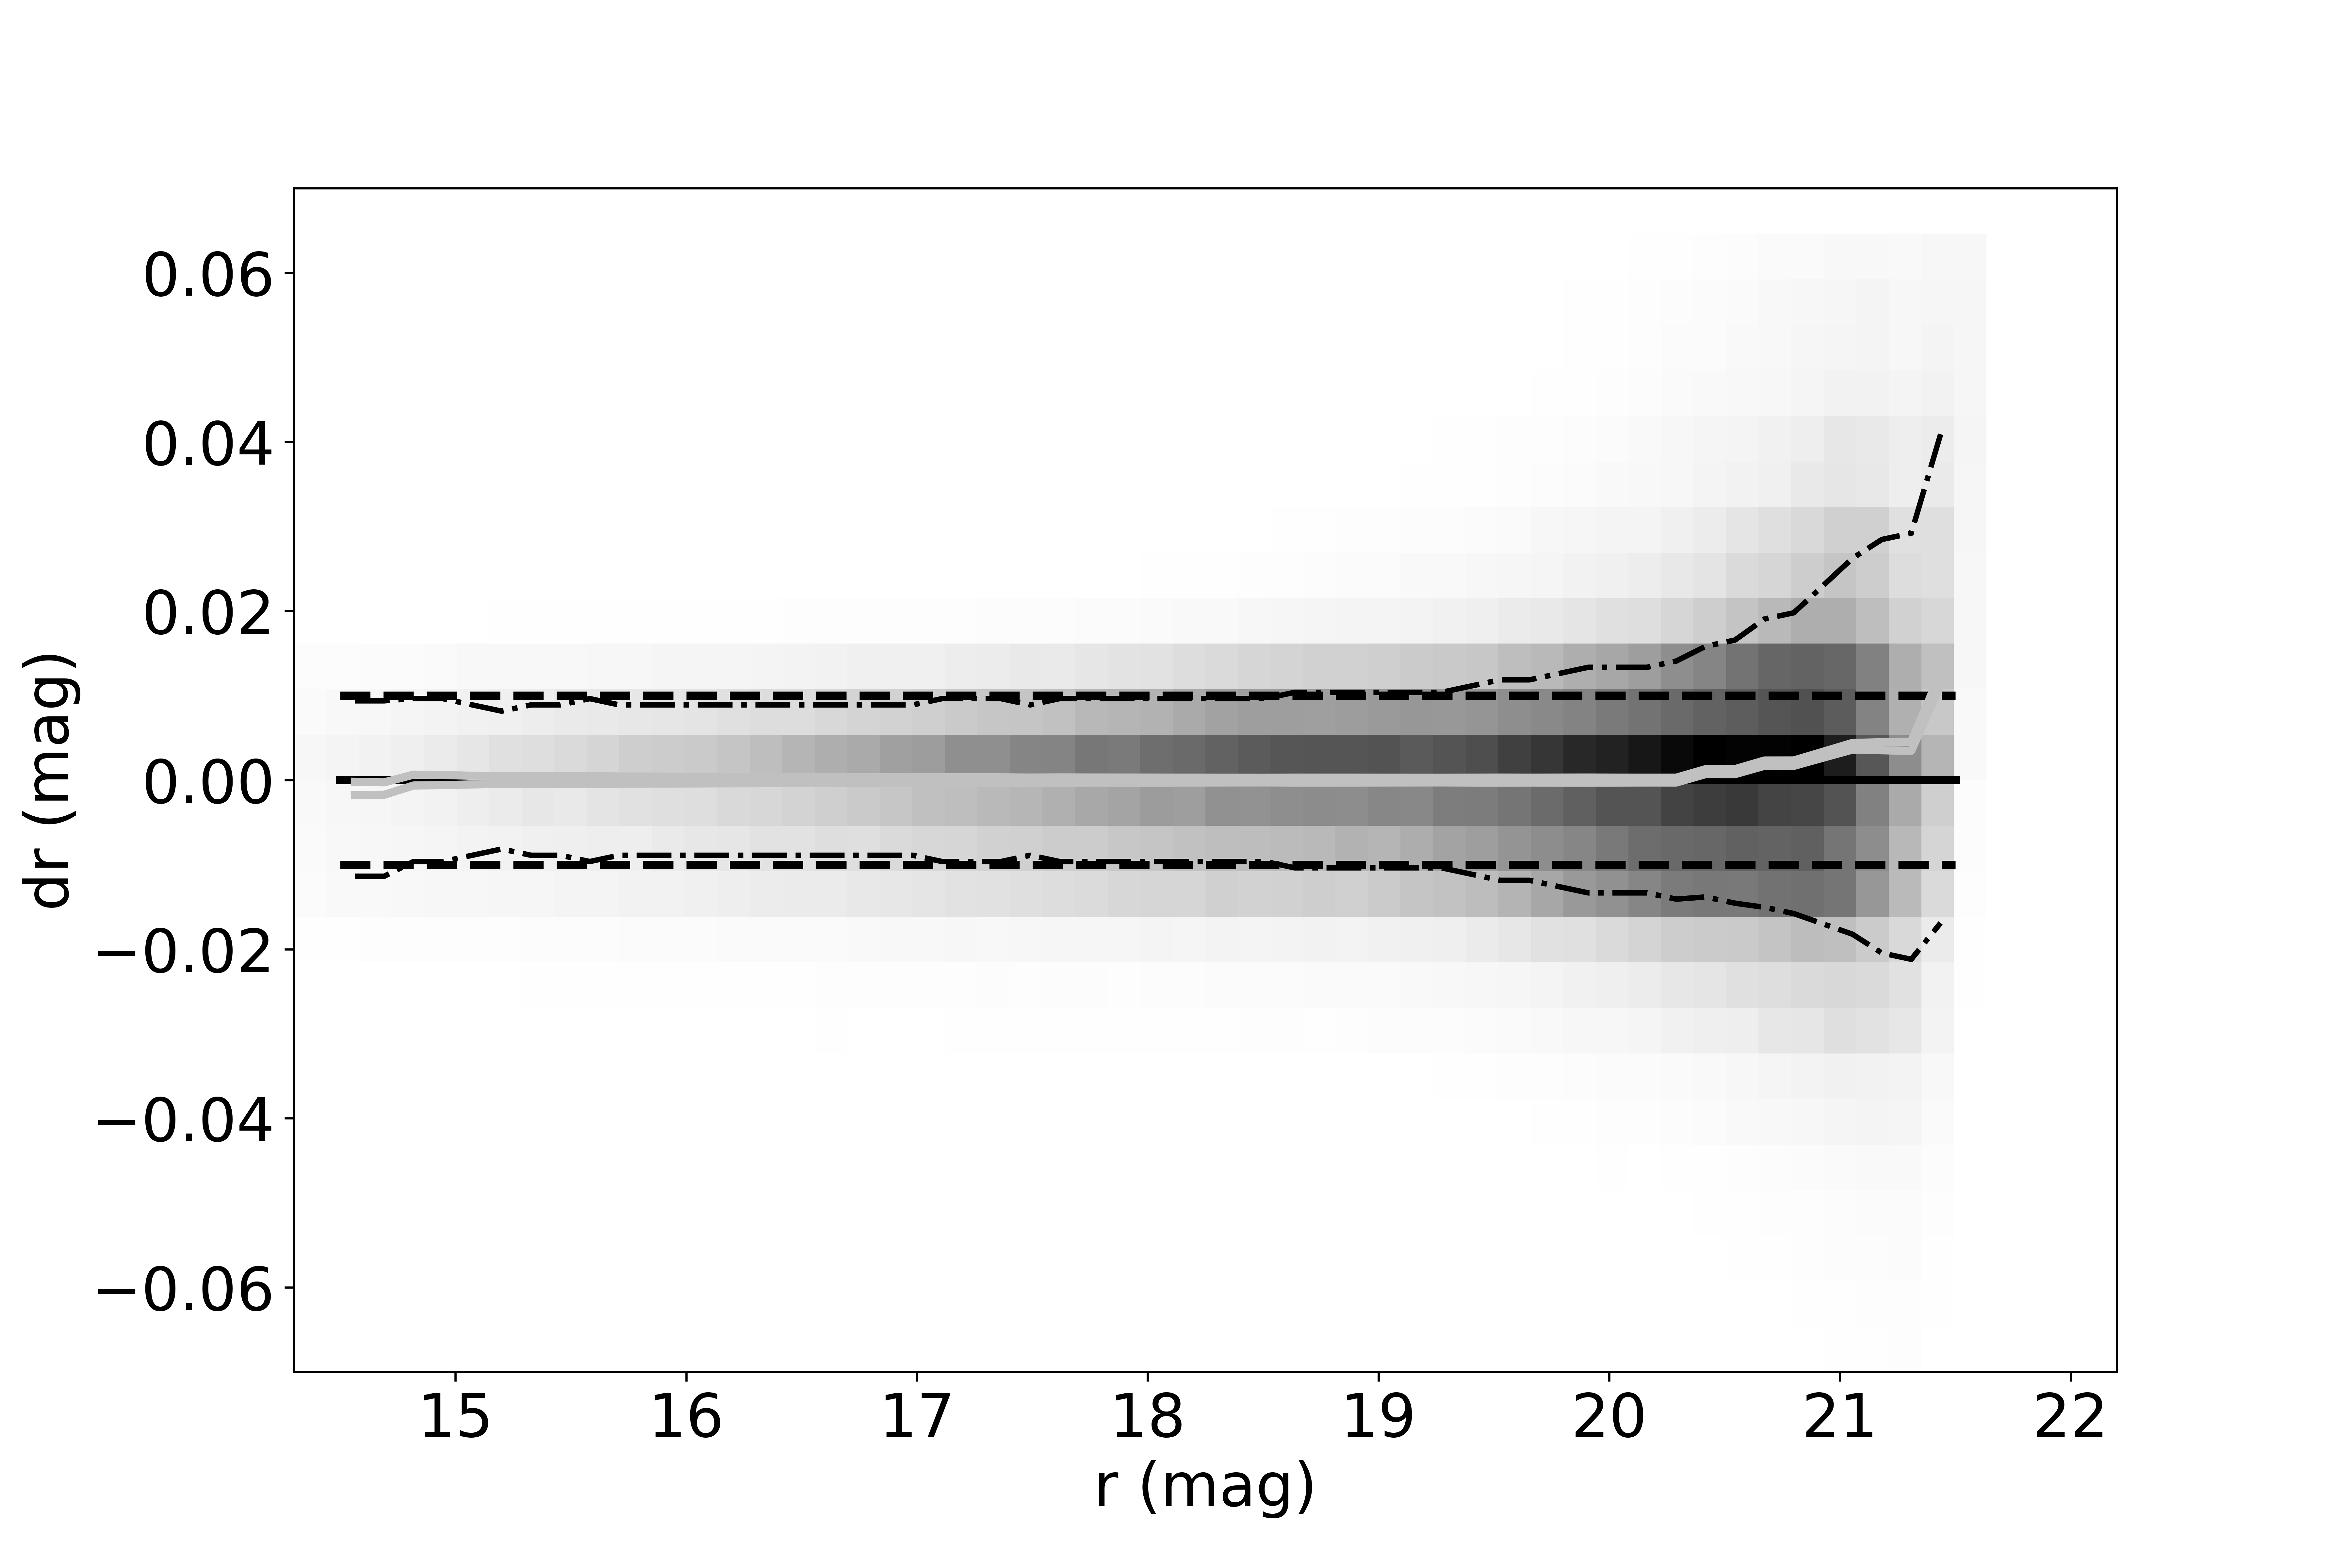
\includegraphics[width=9cm]{figures/testV26vsV33_r_dr_r_mag_Hess.png} 
\caption{Analogous to Figure~\ref{fig:v26v34drDec}, except that here the $r$ band
differences are shown as a function of the $r$ band magnitude. The scatted of median
values per bin is 1.9 millimag. The scatter of individual values is $\sim0.01$ mag
for $r<20$, and it is due to more data in the new catalog.} 
\label{fig:v26v34drr}
\end{figure}


\begin{figure}
    \centering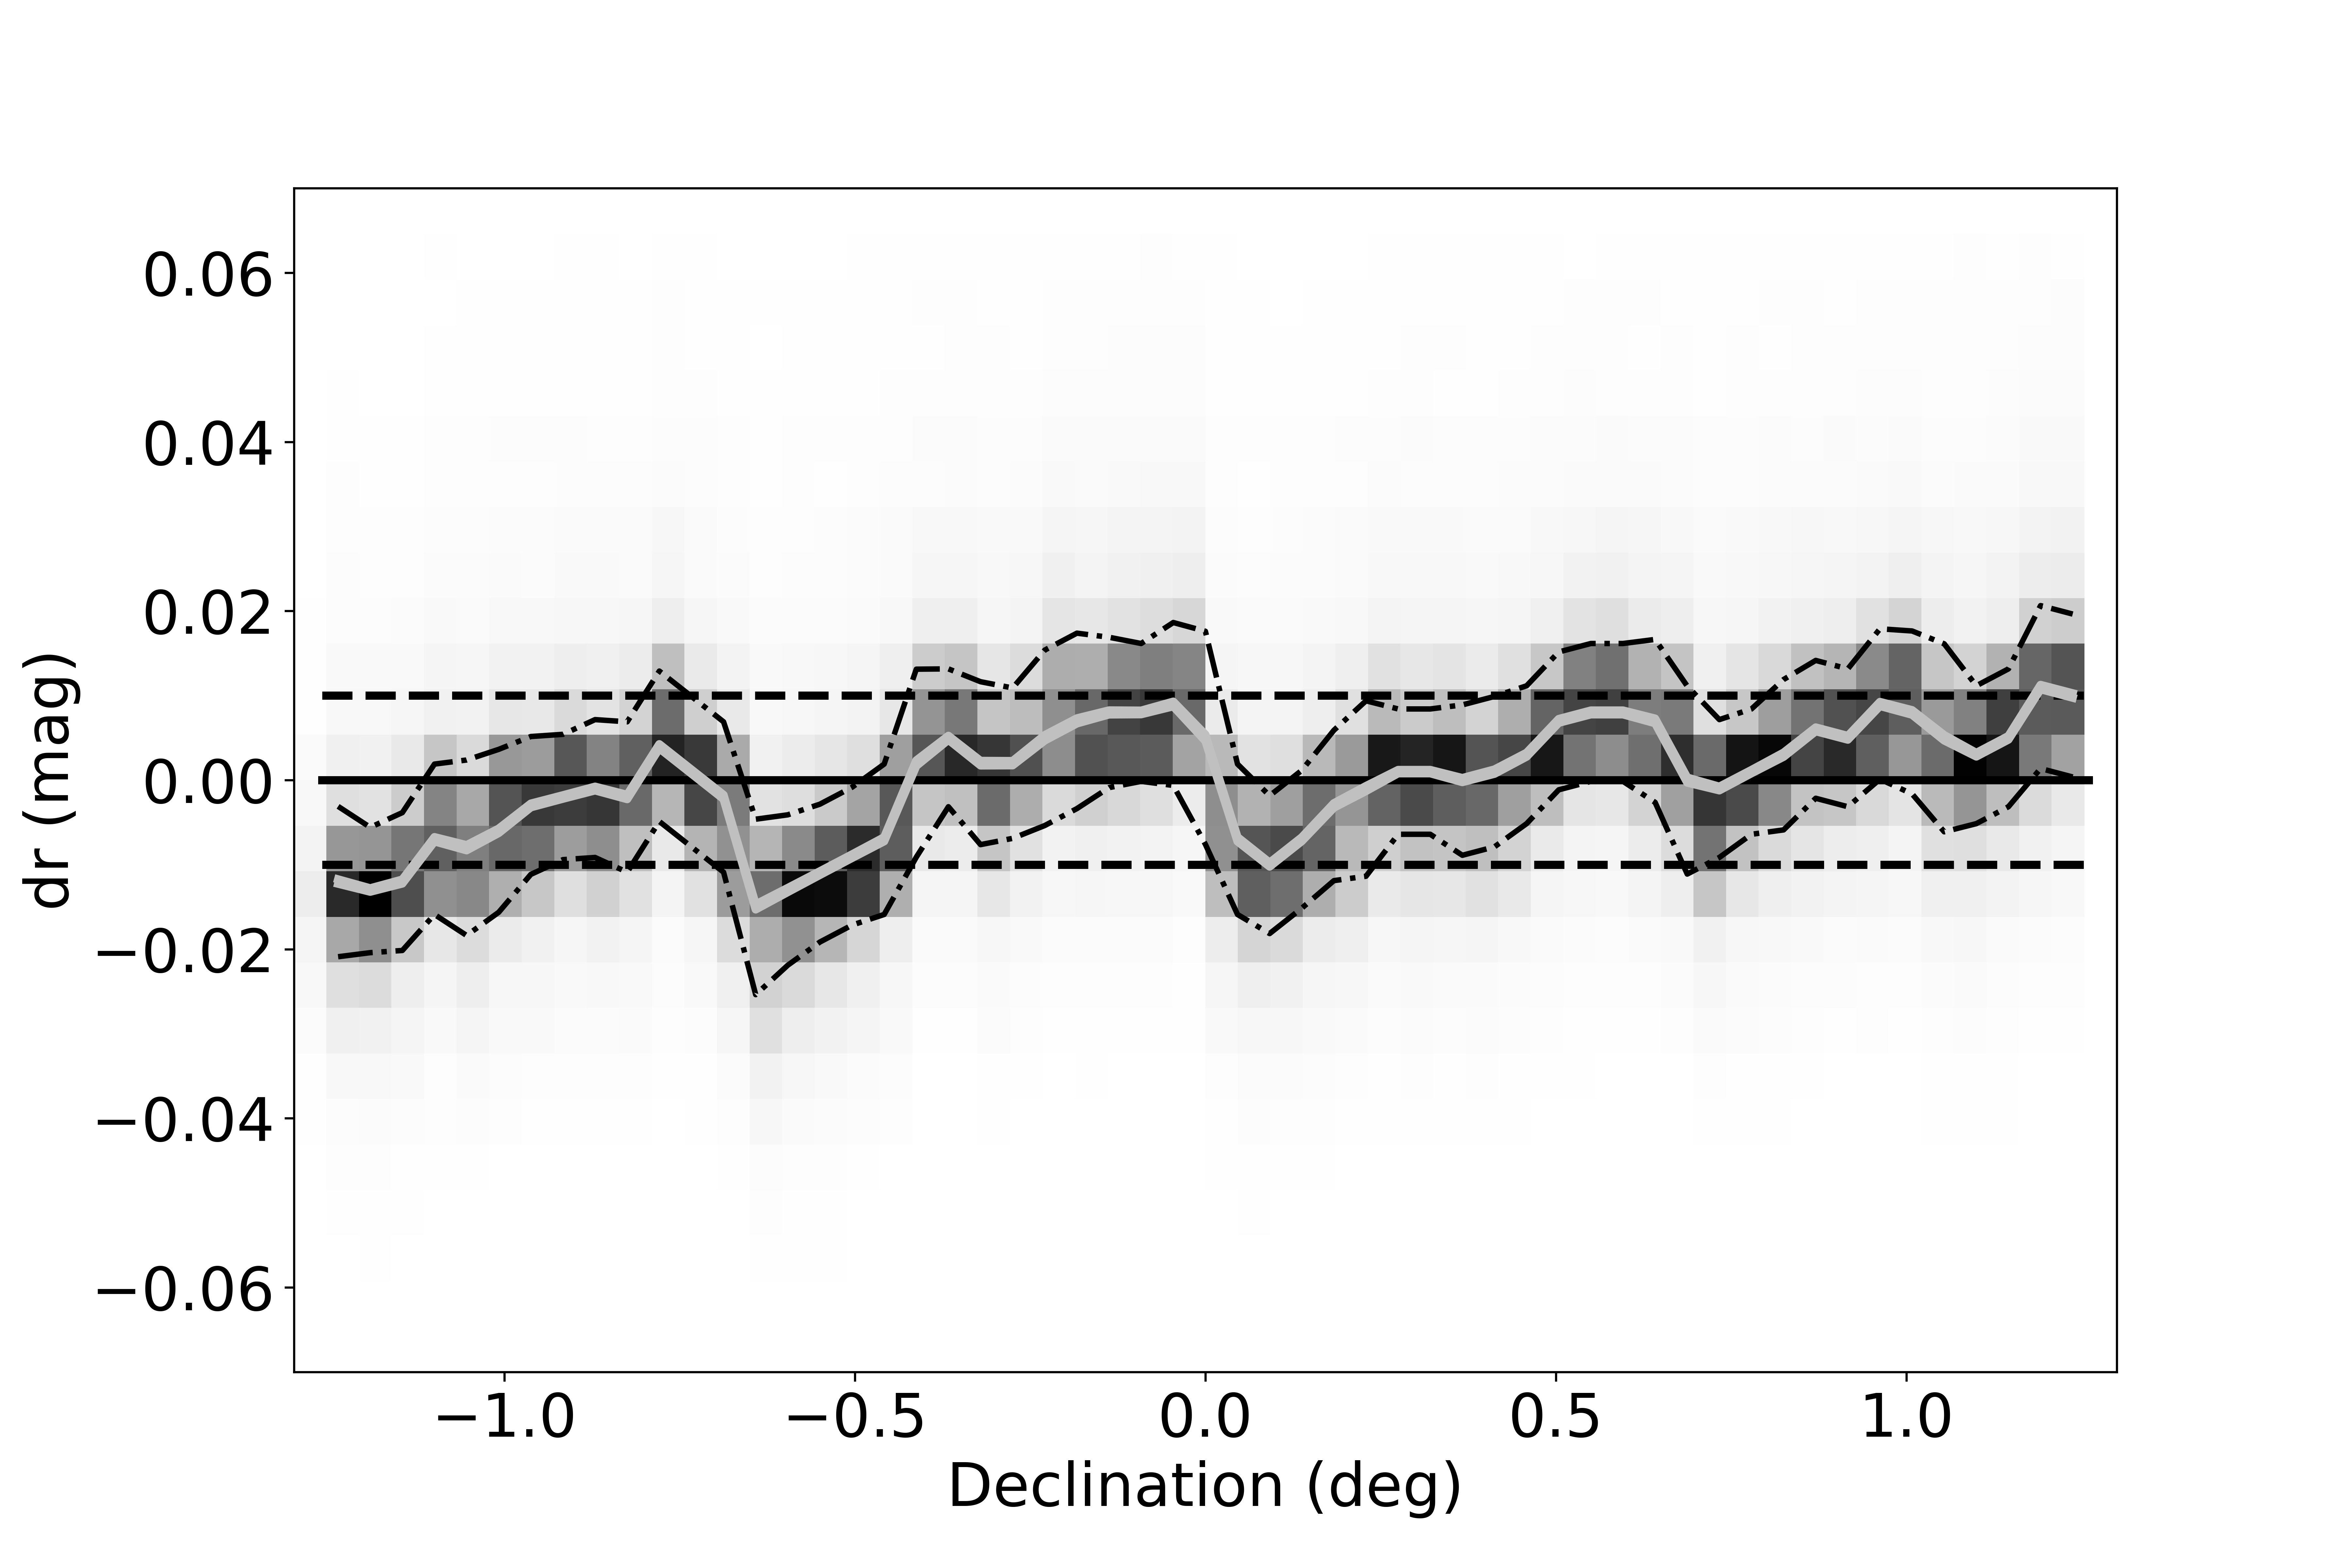
\includegraphics[width=9cm]{figures/testV26vsV33_r_dr_Dec_Hess.png} 
\caption{The differences between $r$ band magnitudes listed in the v2.6 and v3.4 
    SDSS Standard Star catalogs. The size of the four regions corresponds to the
field-of-view size of the SDSS Photometric Calibration Telescope. The standard 
deviation for median values per bin is 6.8 millimag, with extreme values about 0.01 mag. 
The scatter of binned medians in R.A. direction is much smaller -- 2.0 millimag. 
For statistics in other bands, please see Table~\ref{tab:oldnewRMS}.}
\label{fig:v26v34drDec}
\end{figure}
 

\begin{figure}
    \centering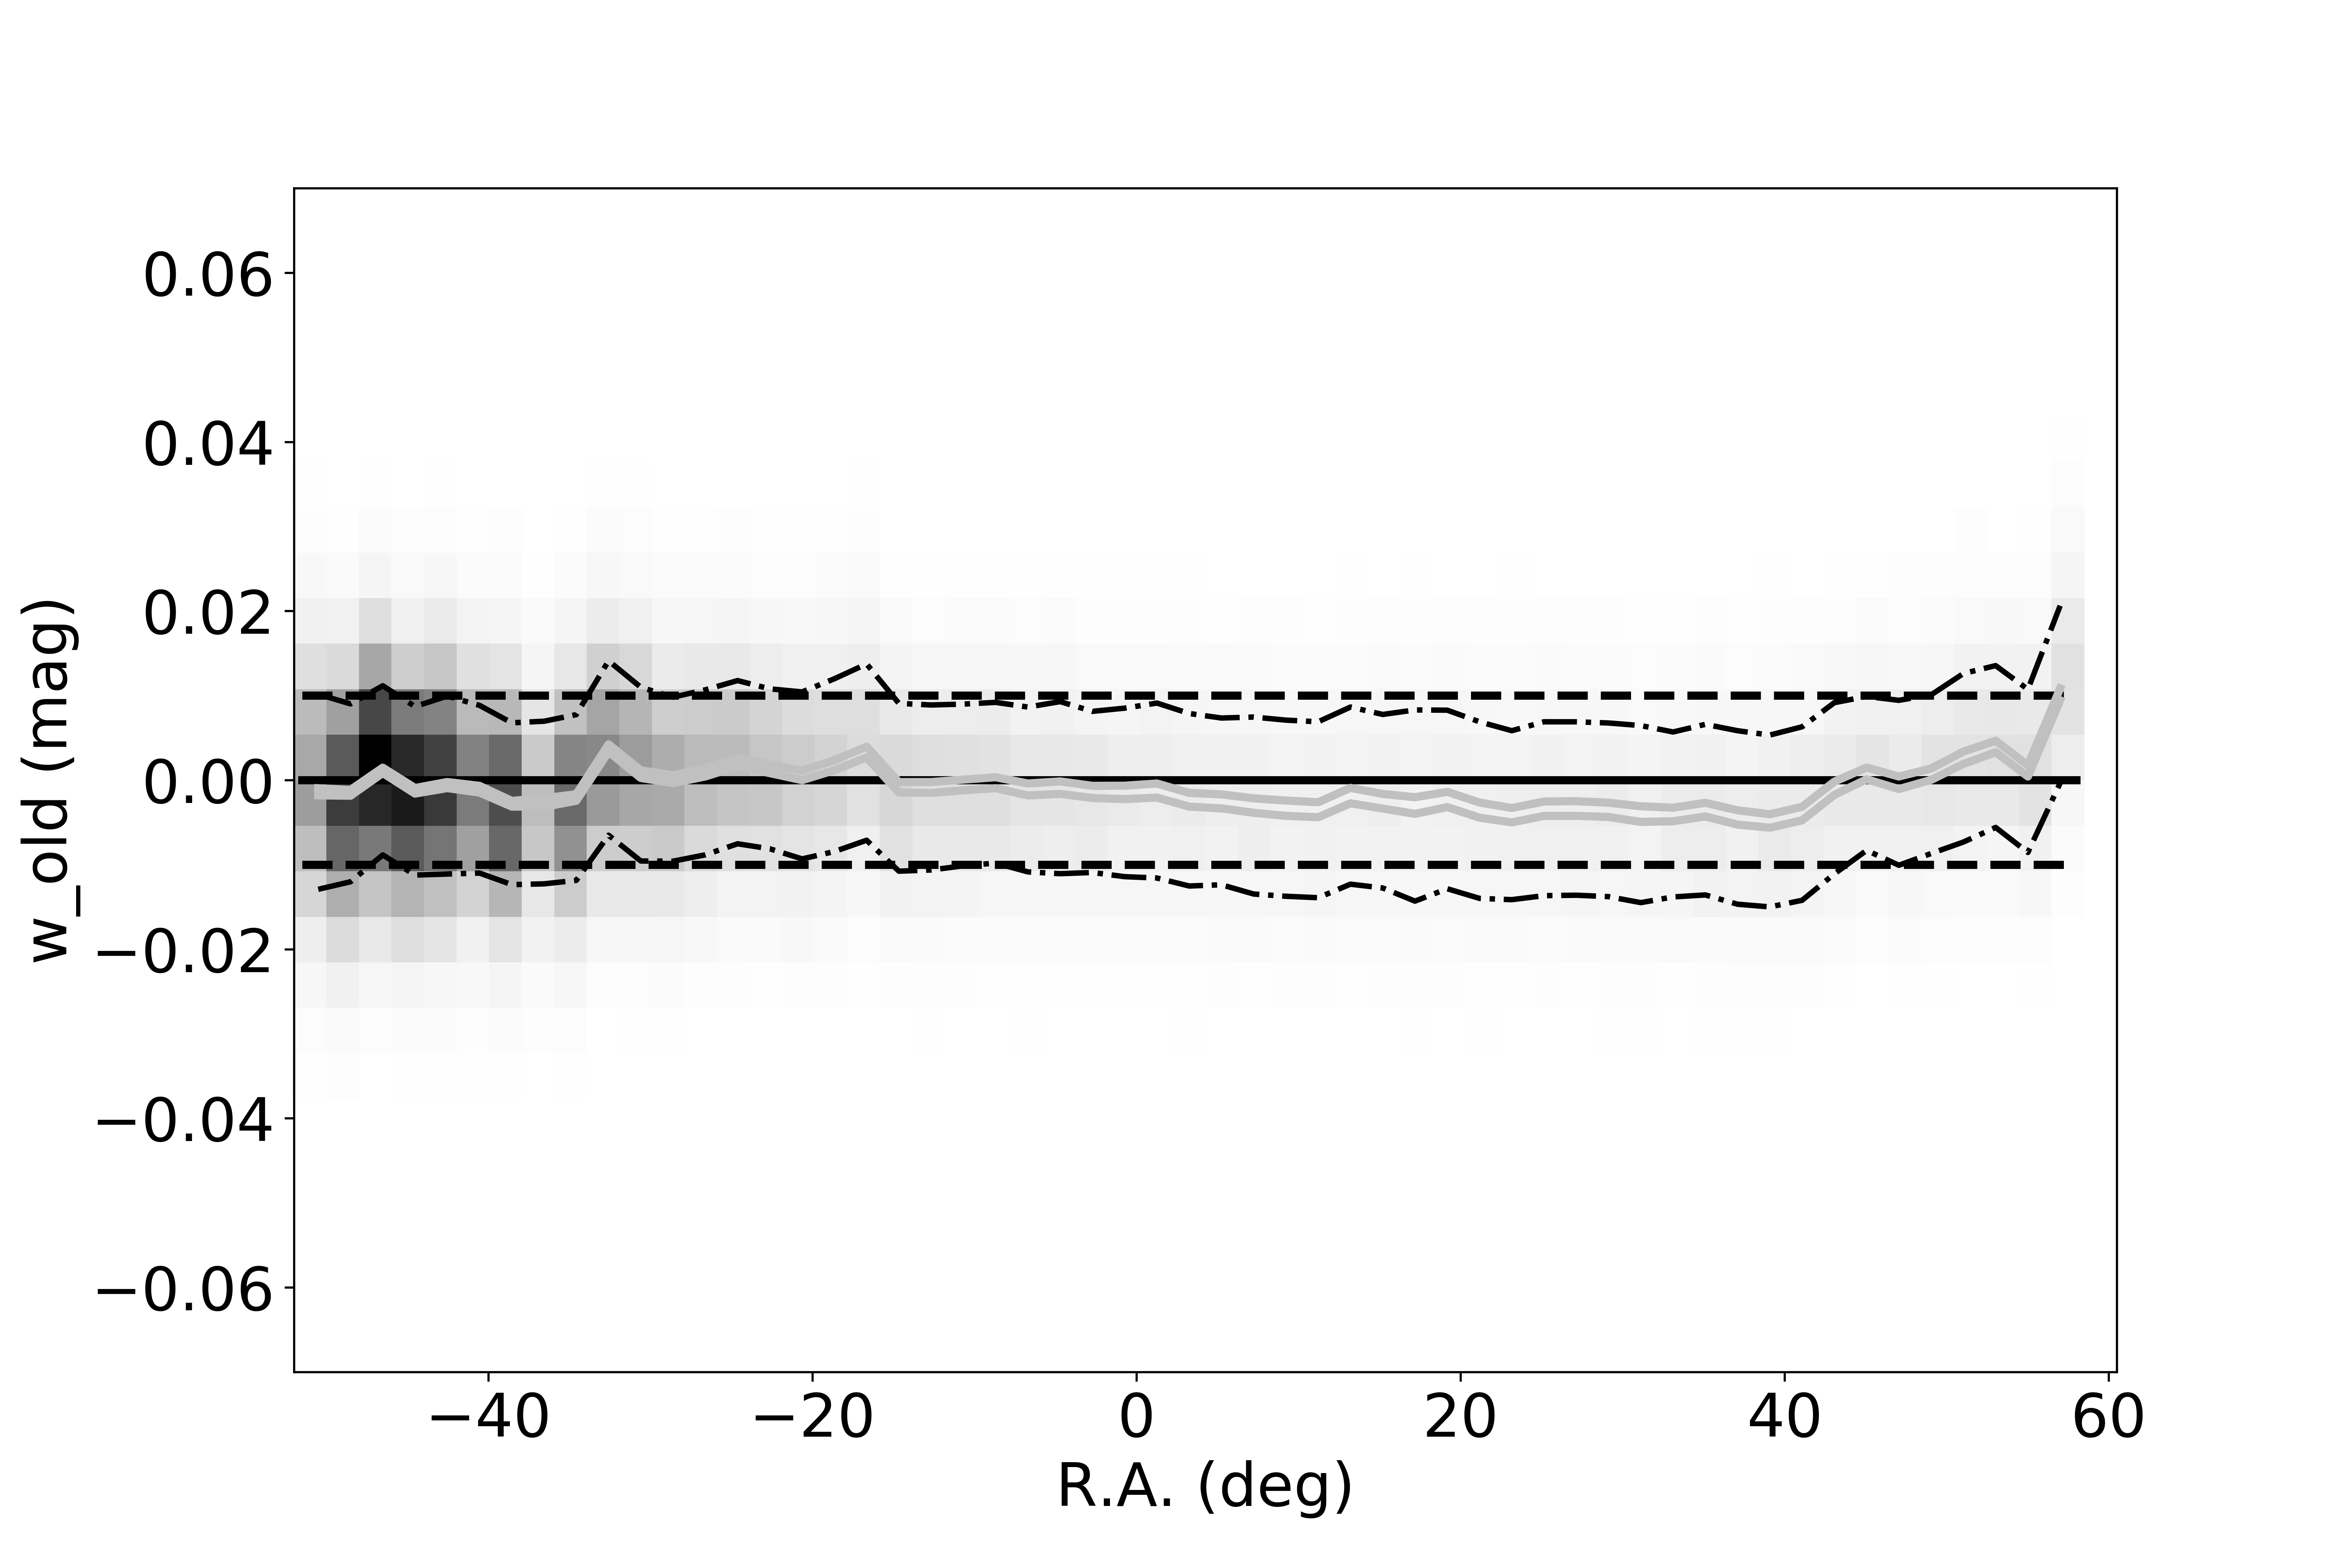
\includegraphics[width=7cm]{figures/testV26vsV33_r_w_old_RA_Hess.png}
    \centering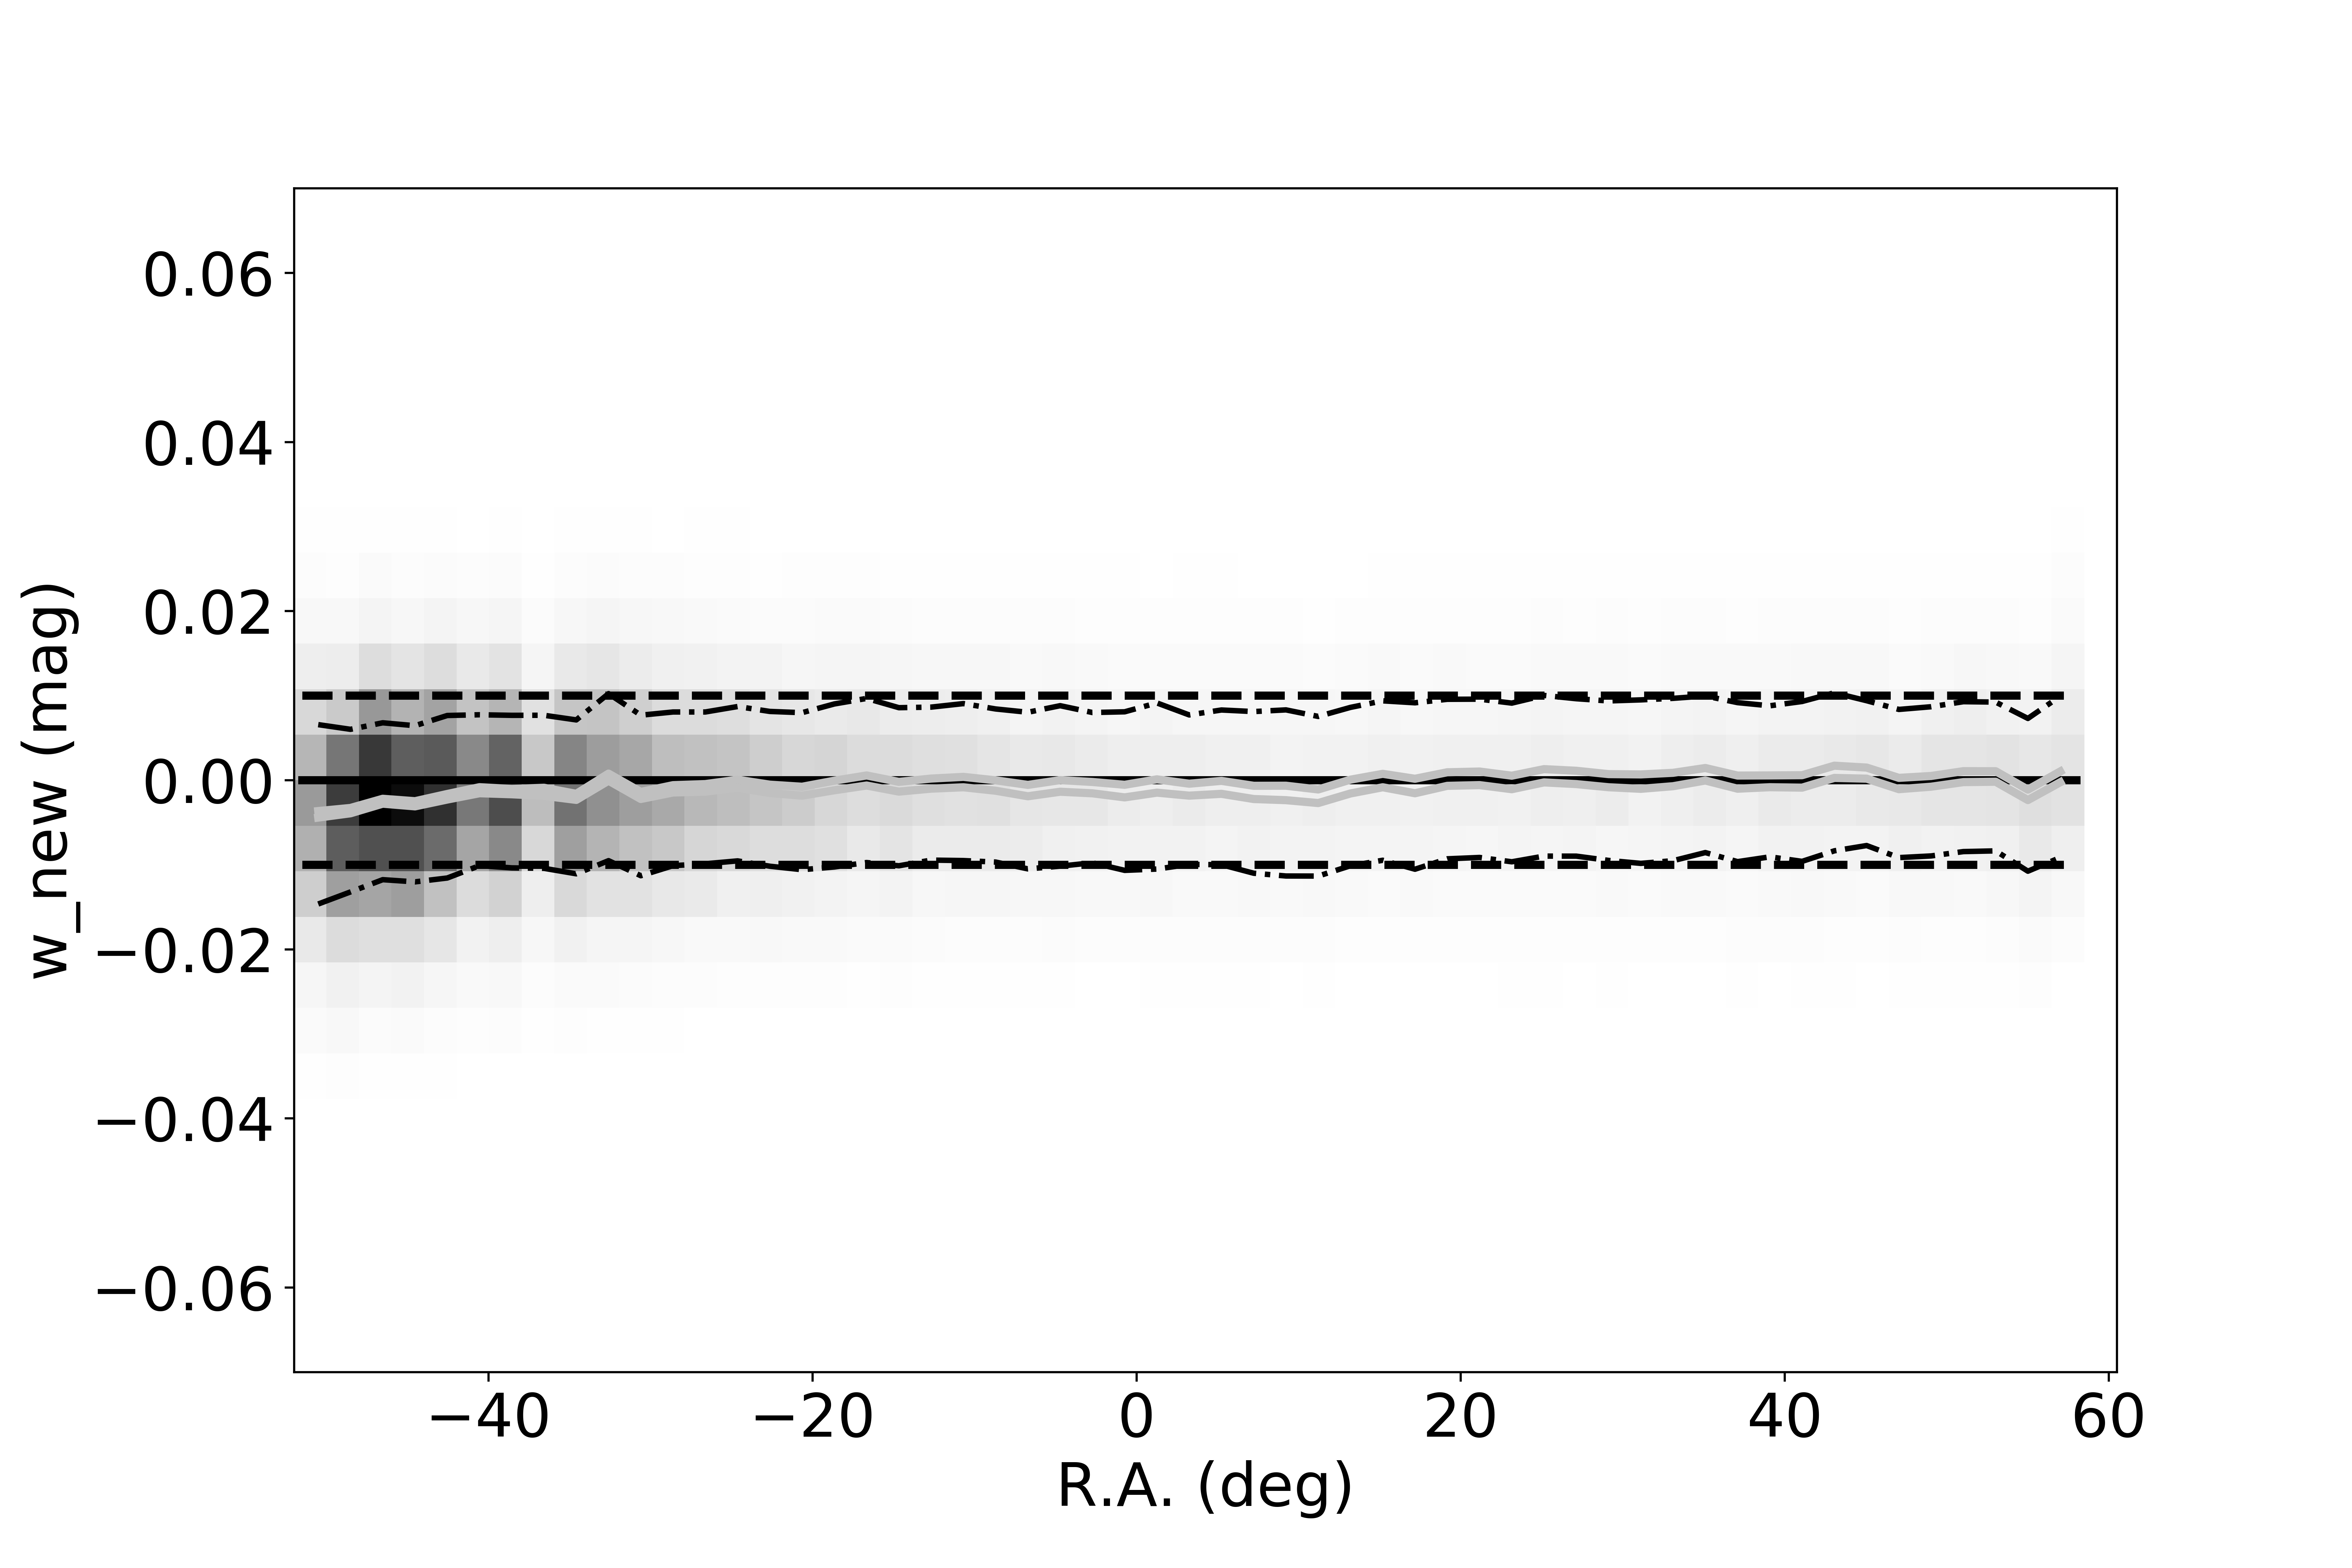
\includegraphics[width=7cm]{figures/testV26vsV33_r_w_new_RA_Hess.png}
    \centering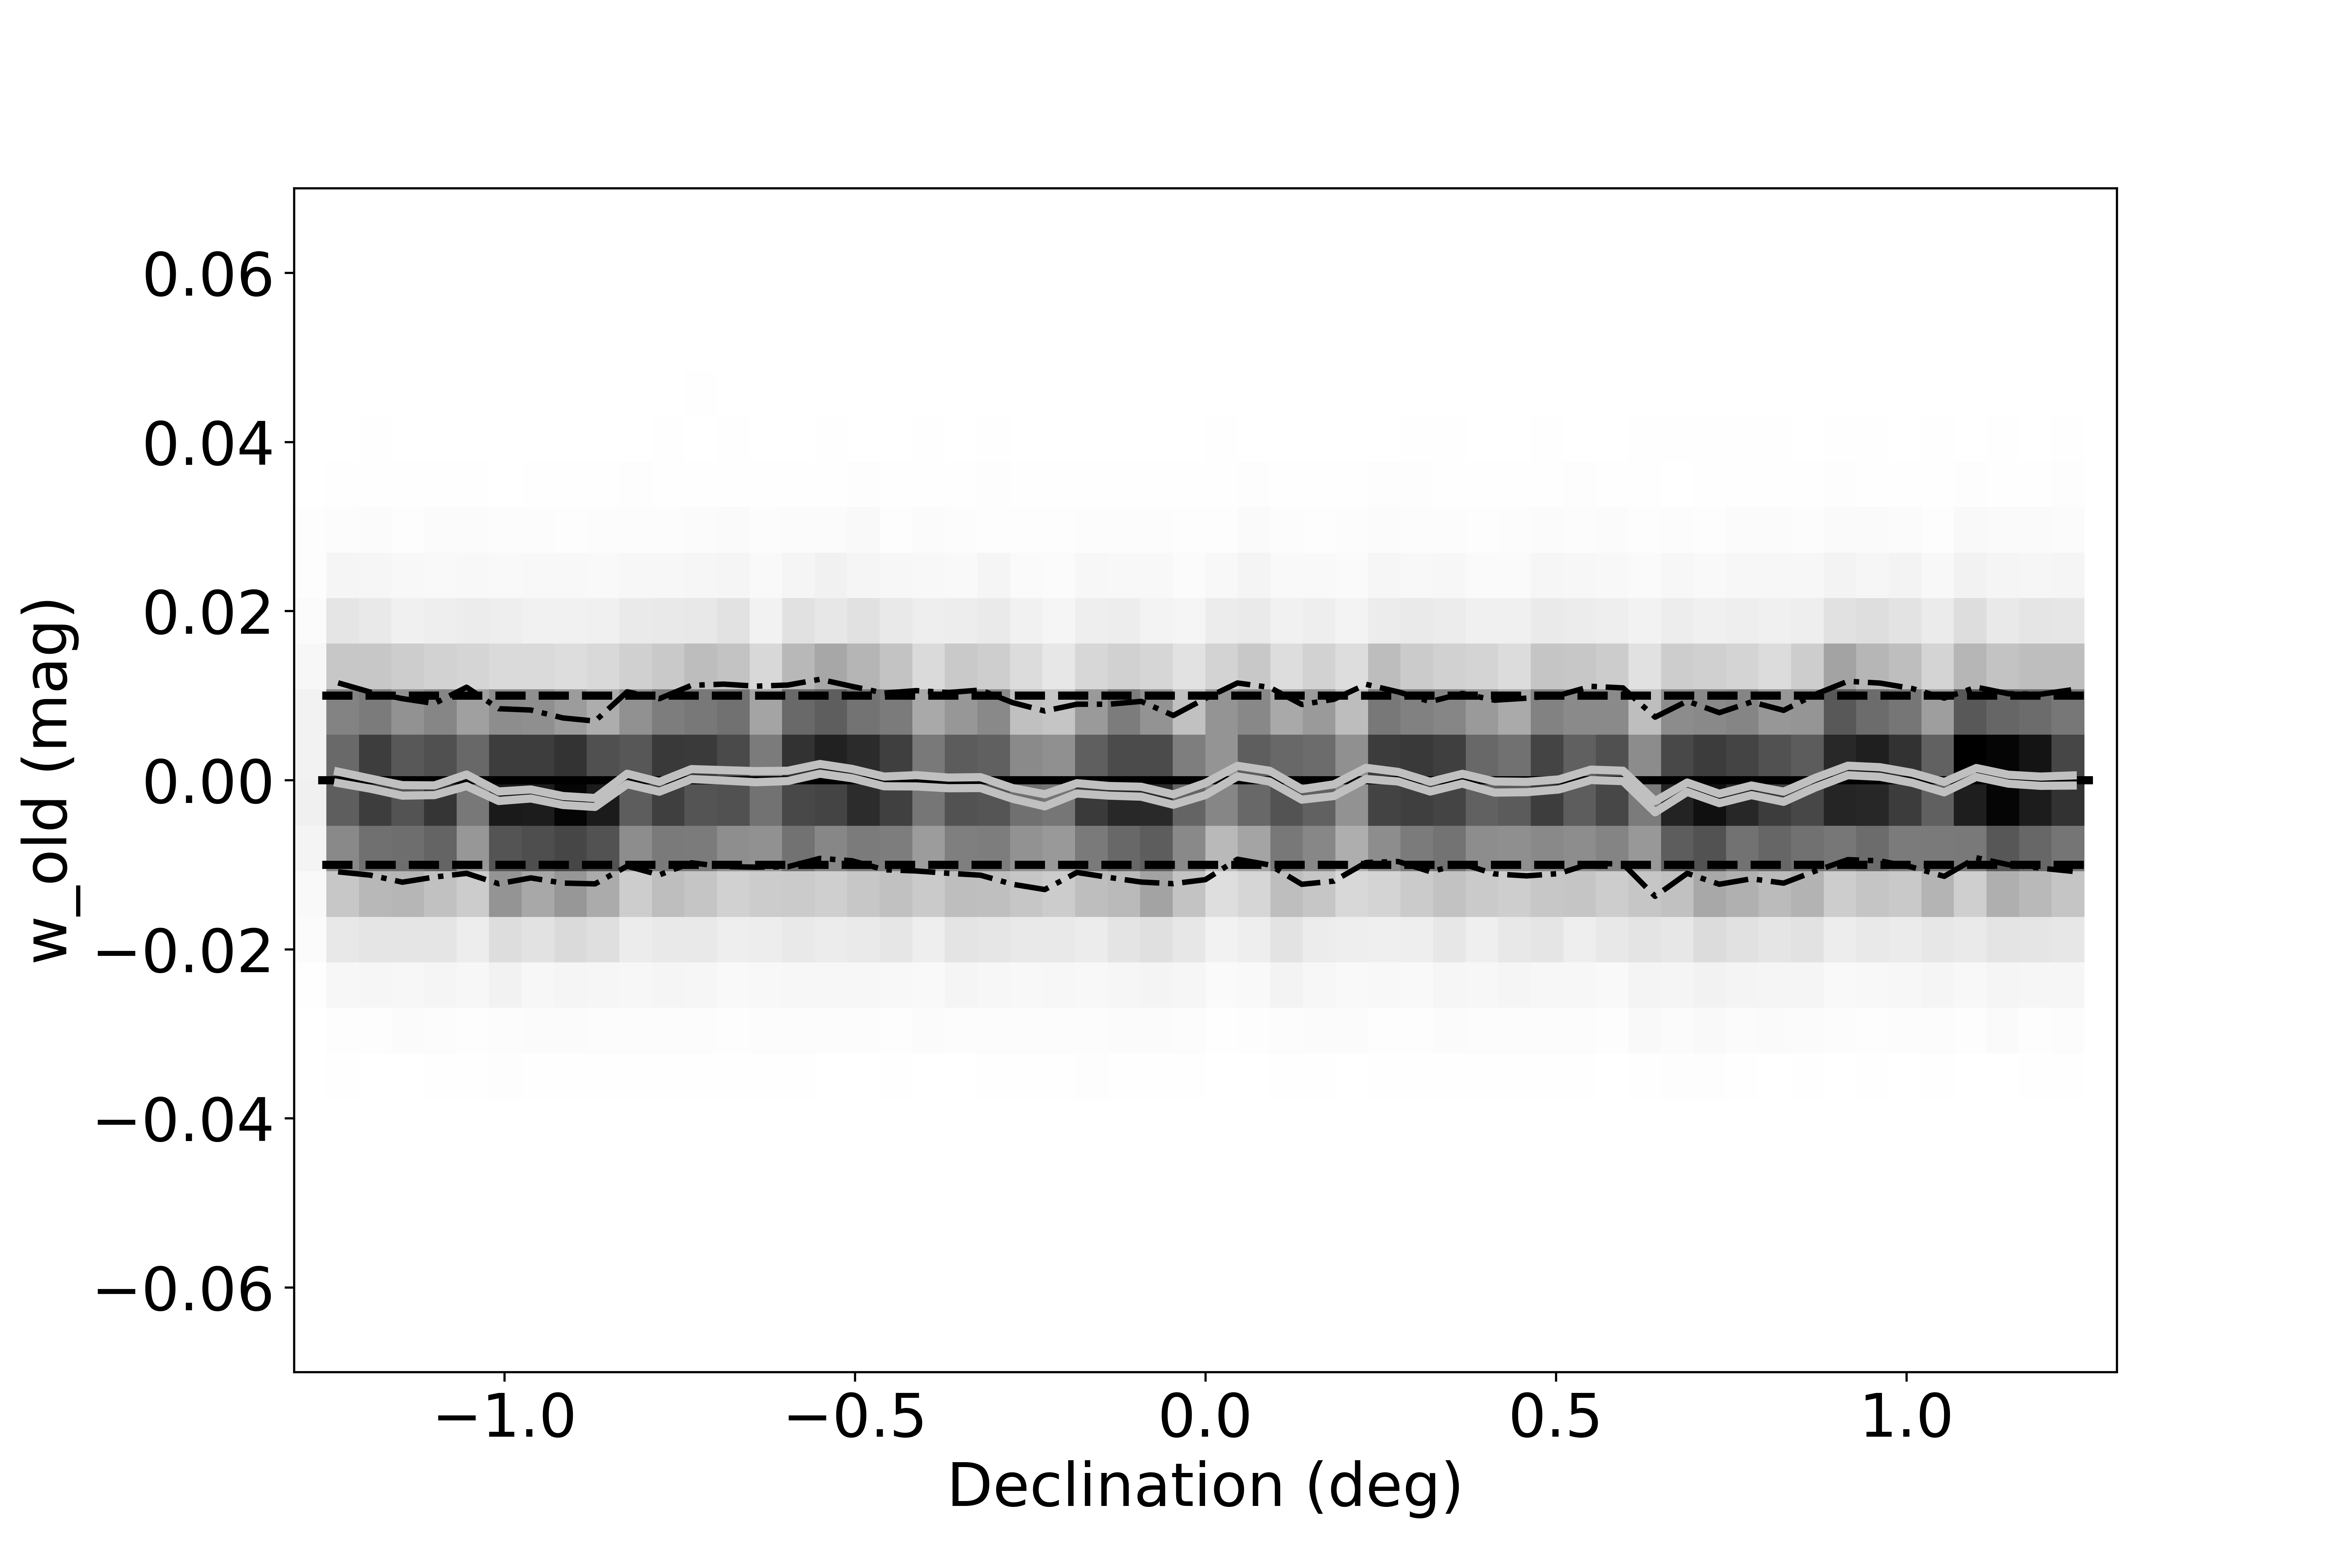
\includegraphics[width=7cm]{figures/testV26vsV33_r_w_old_Dec_Hess.png}
    \centering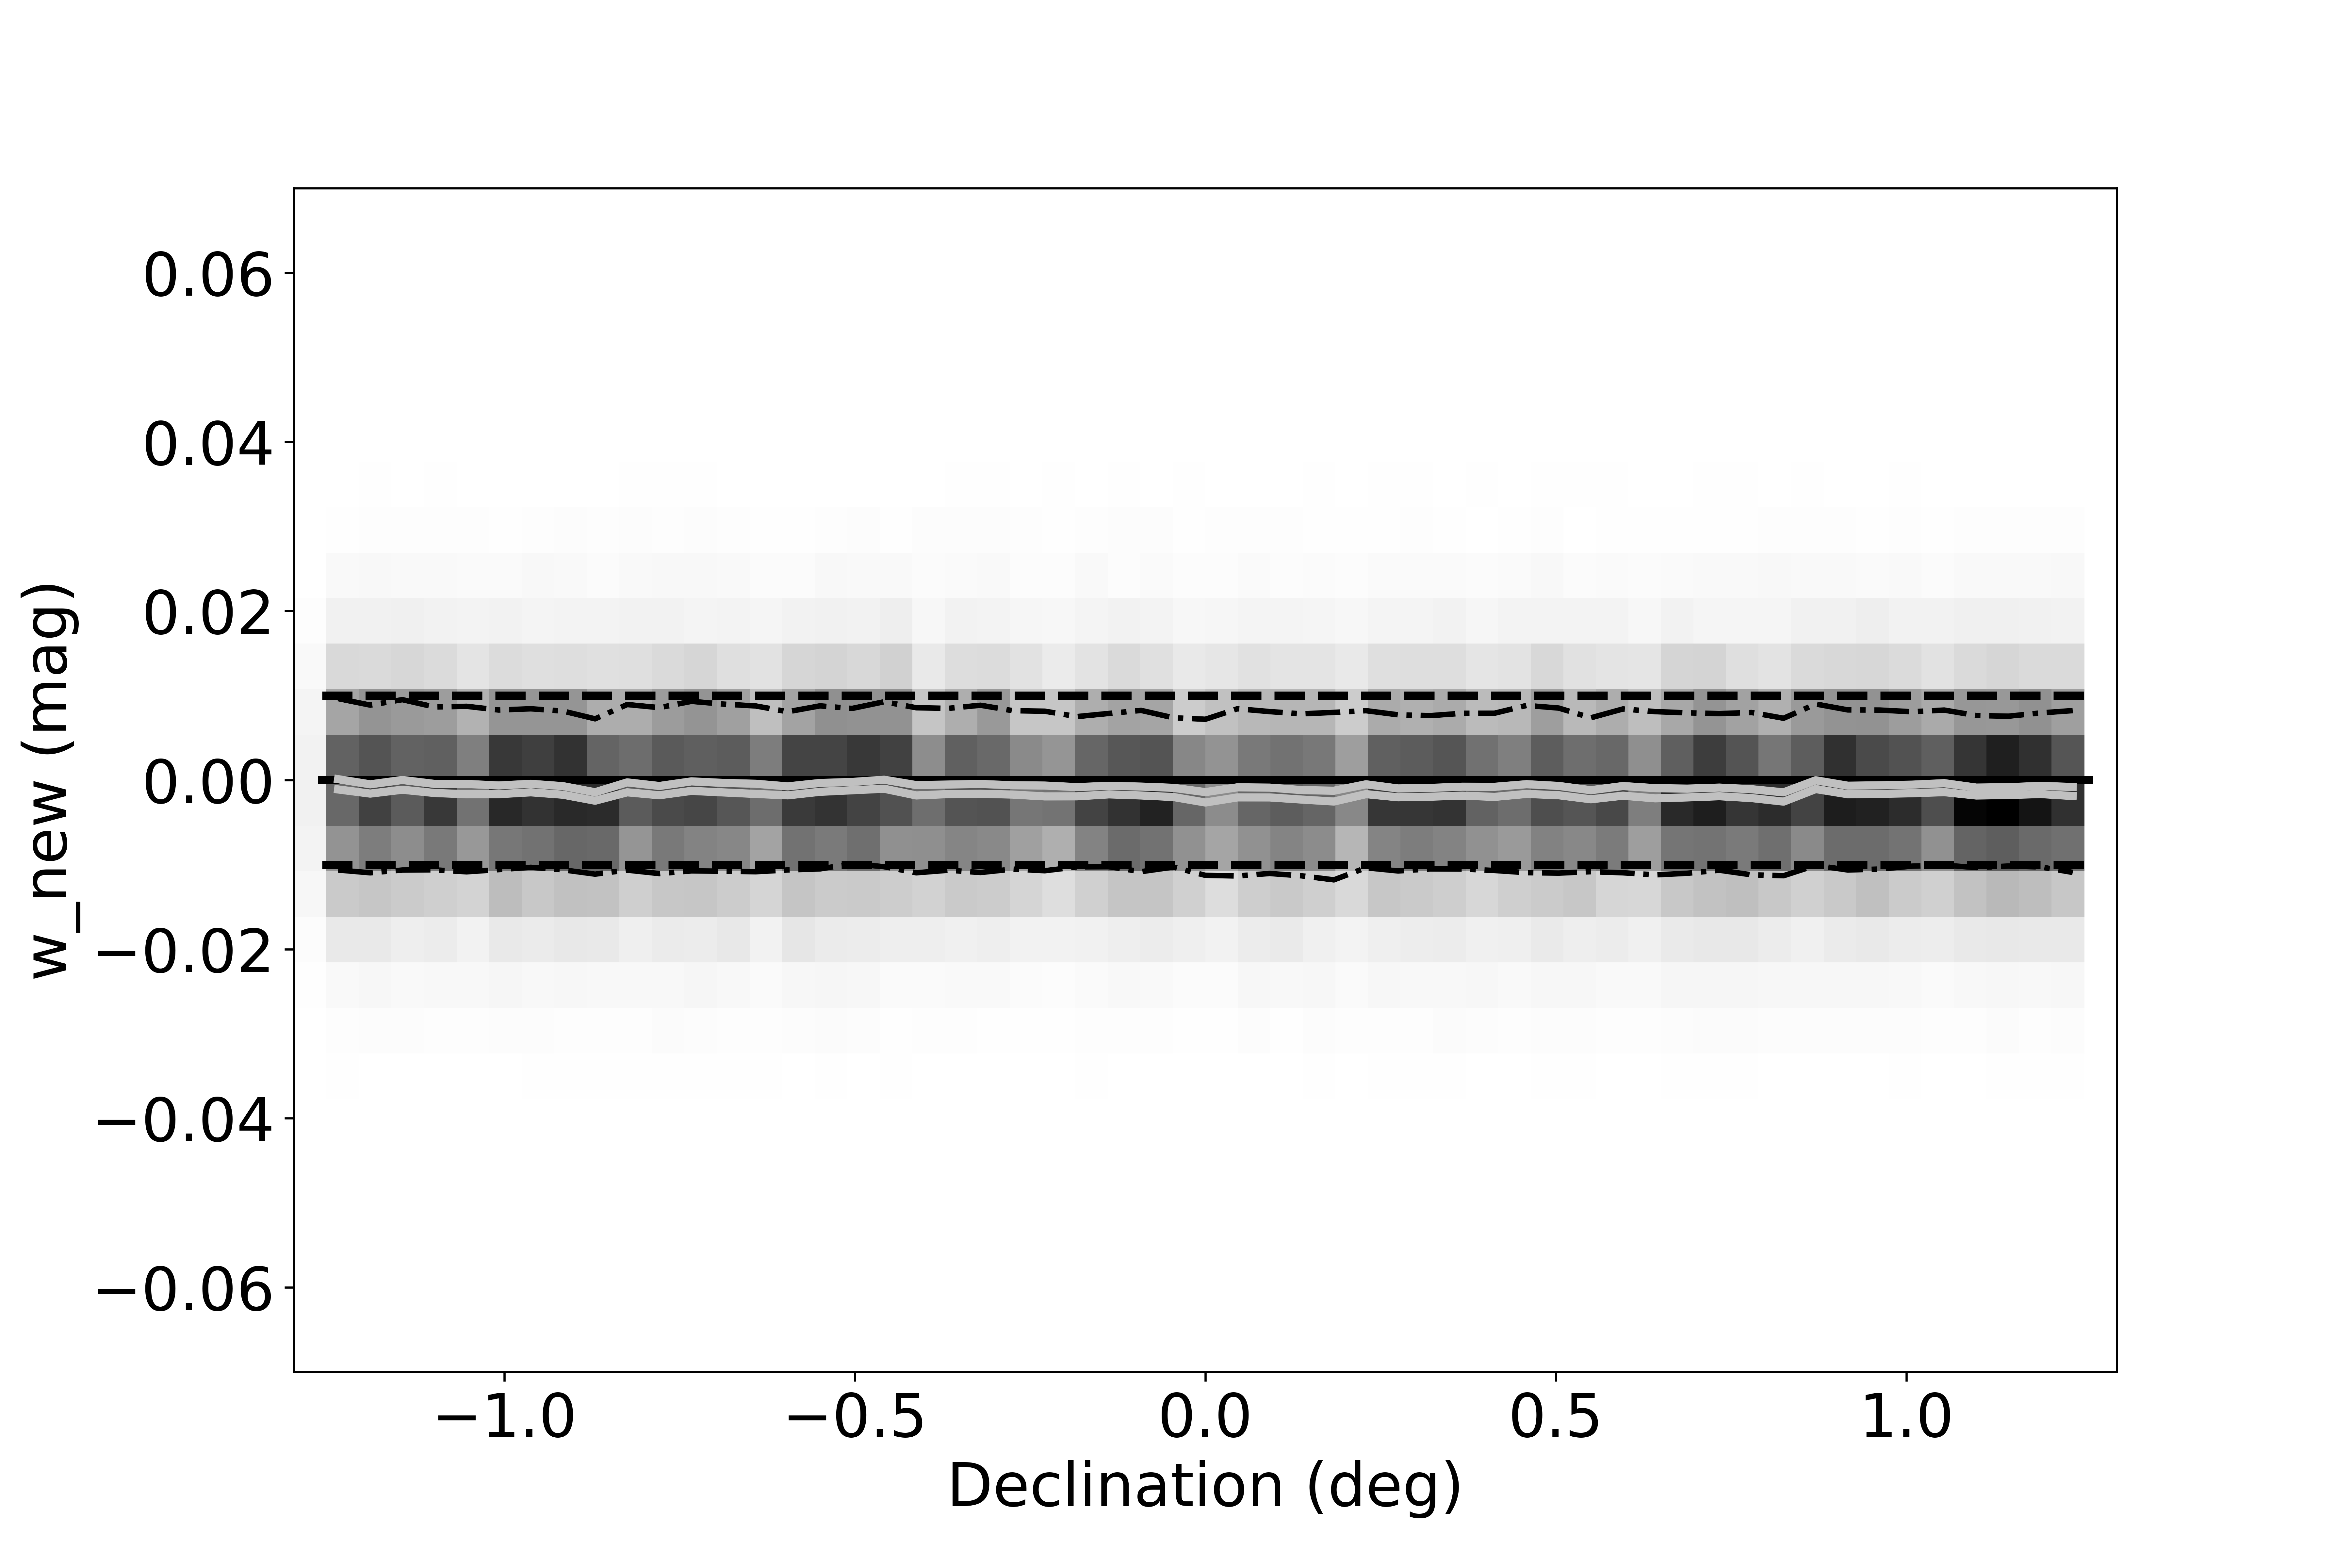
\includegraphics[width=7cm]{figures/testV26vsV33_r_w_new_Dec_Hess.png}
\caption{A comparison of the $w$ color, the second principal color in the SDSS
$r-i$ vs. $g-r$ color-color diagram, behavior for the v2.6 (left) and v3.4 (right)
catalogs. The standard deviation of the median $w$ values binned by R.A. and Dec
is 2.6 millimag and 1.1 millimag for v2.6 and 1.0 millimag and 0.3 millimag for v3.4,
respectively.}
\label{fig:comparew} 
\end{figure}
 

\begin{figure}
    \centering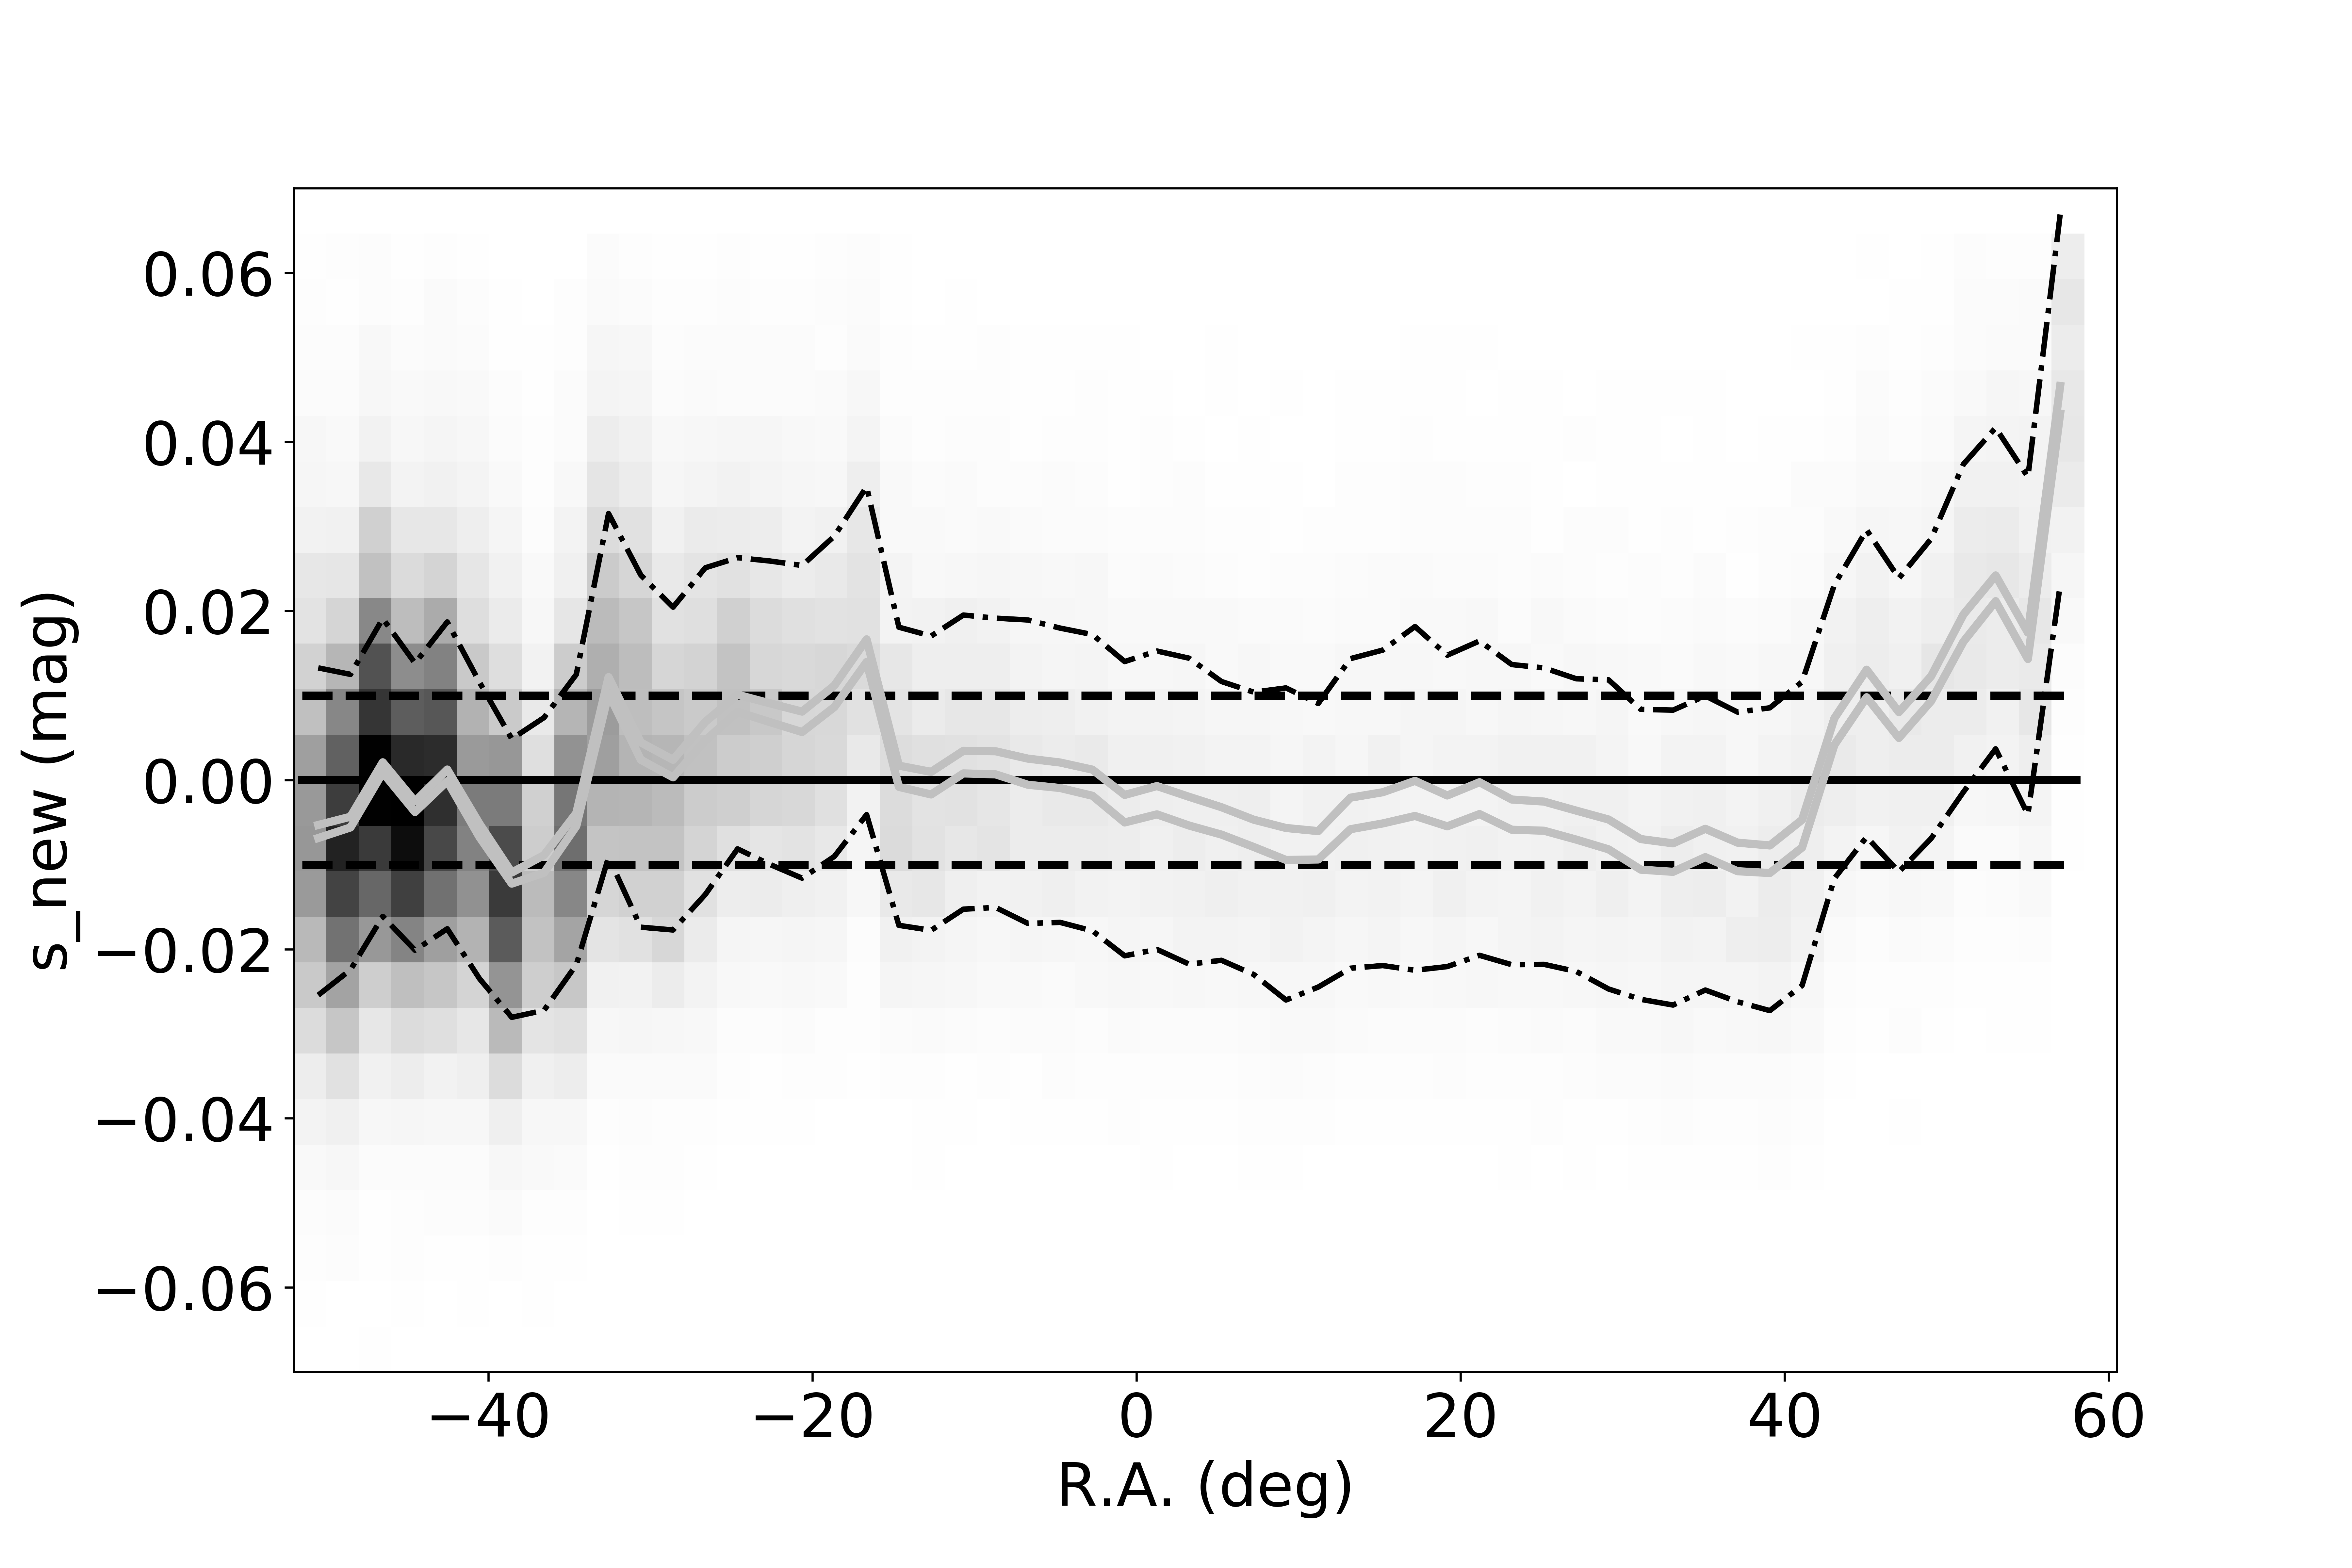
\includegraphics[width=7cm]{figures/testV26vsV33_snew_u_s_new_RA_Hess.png}
    \centering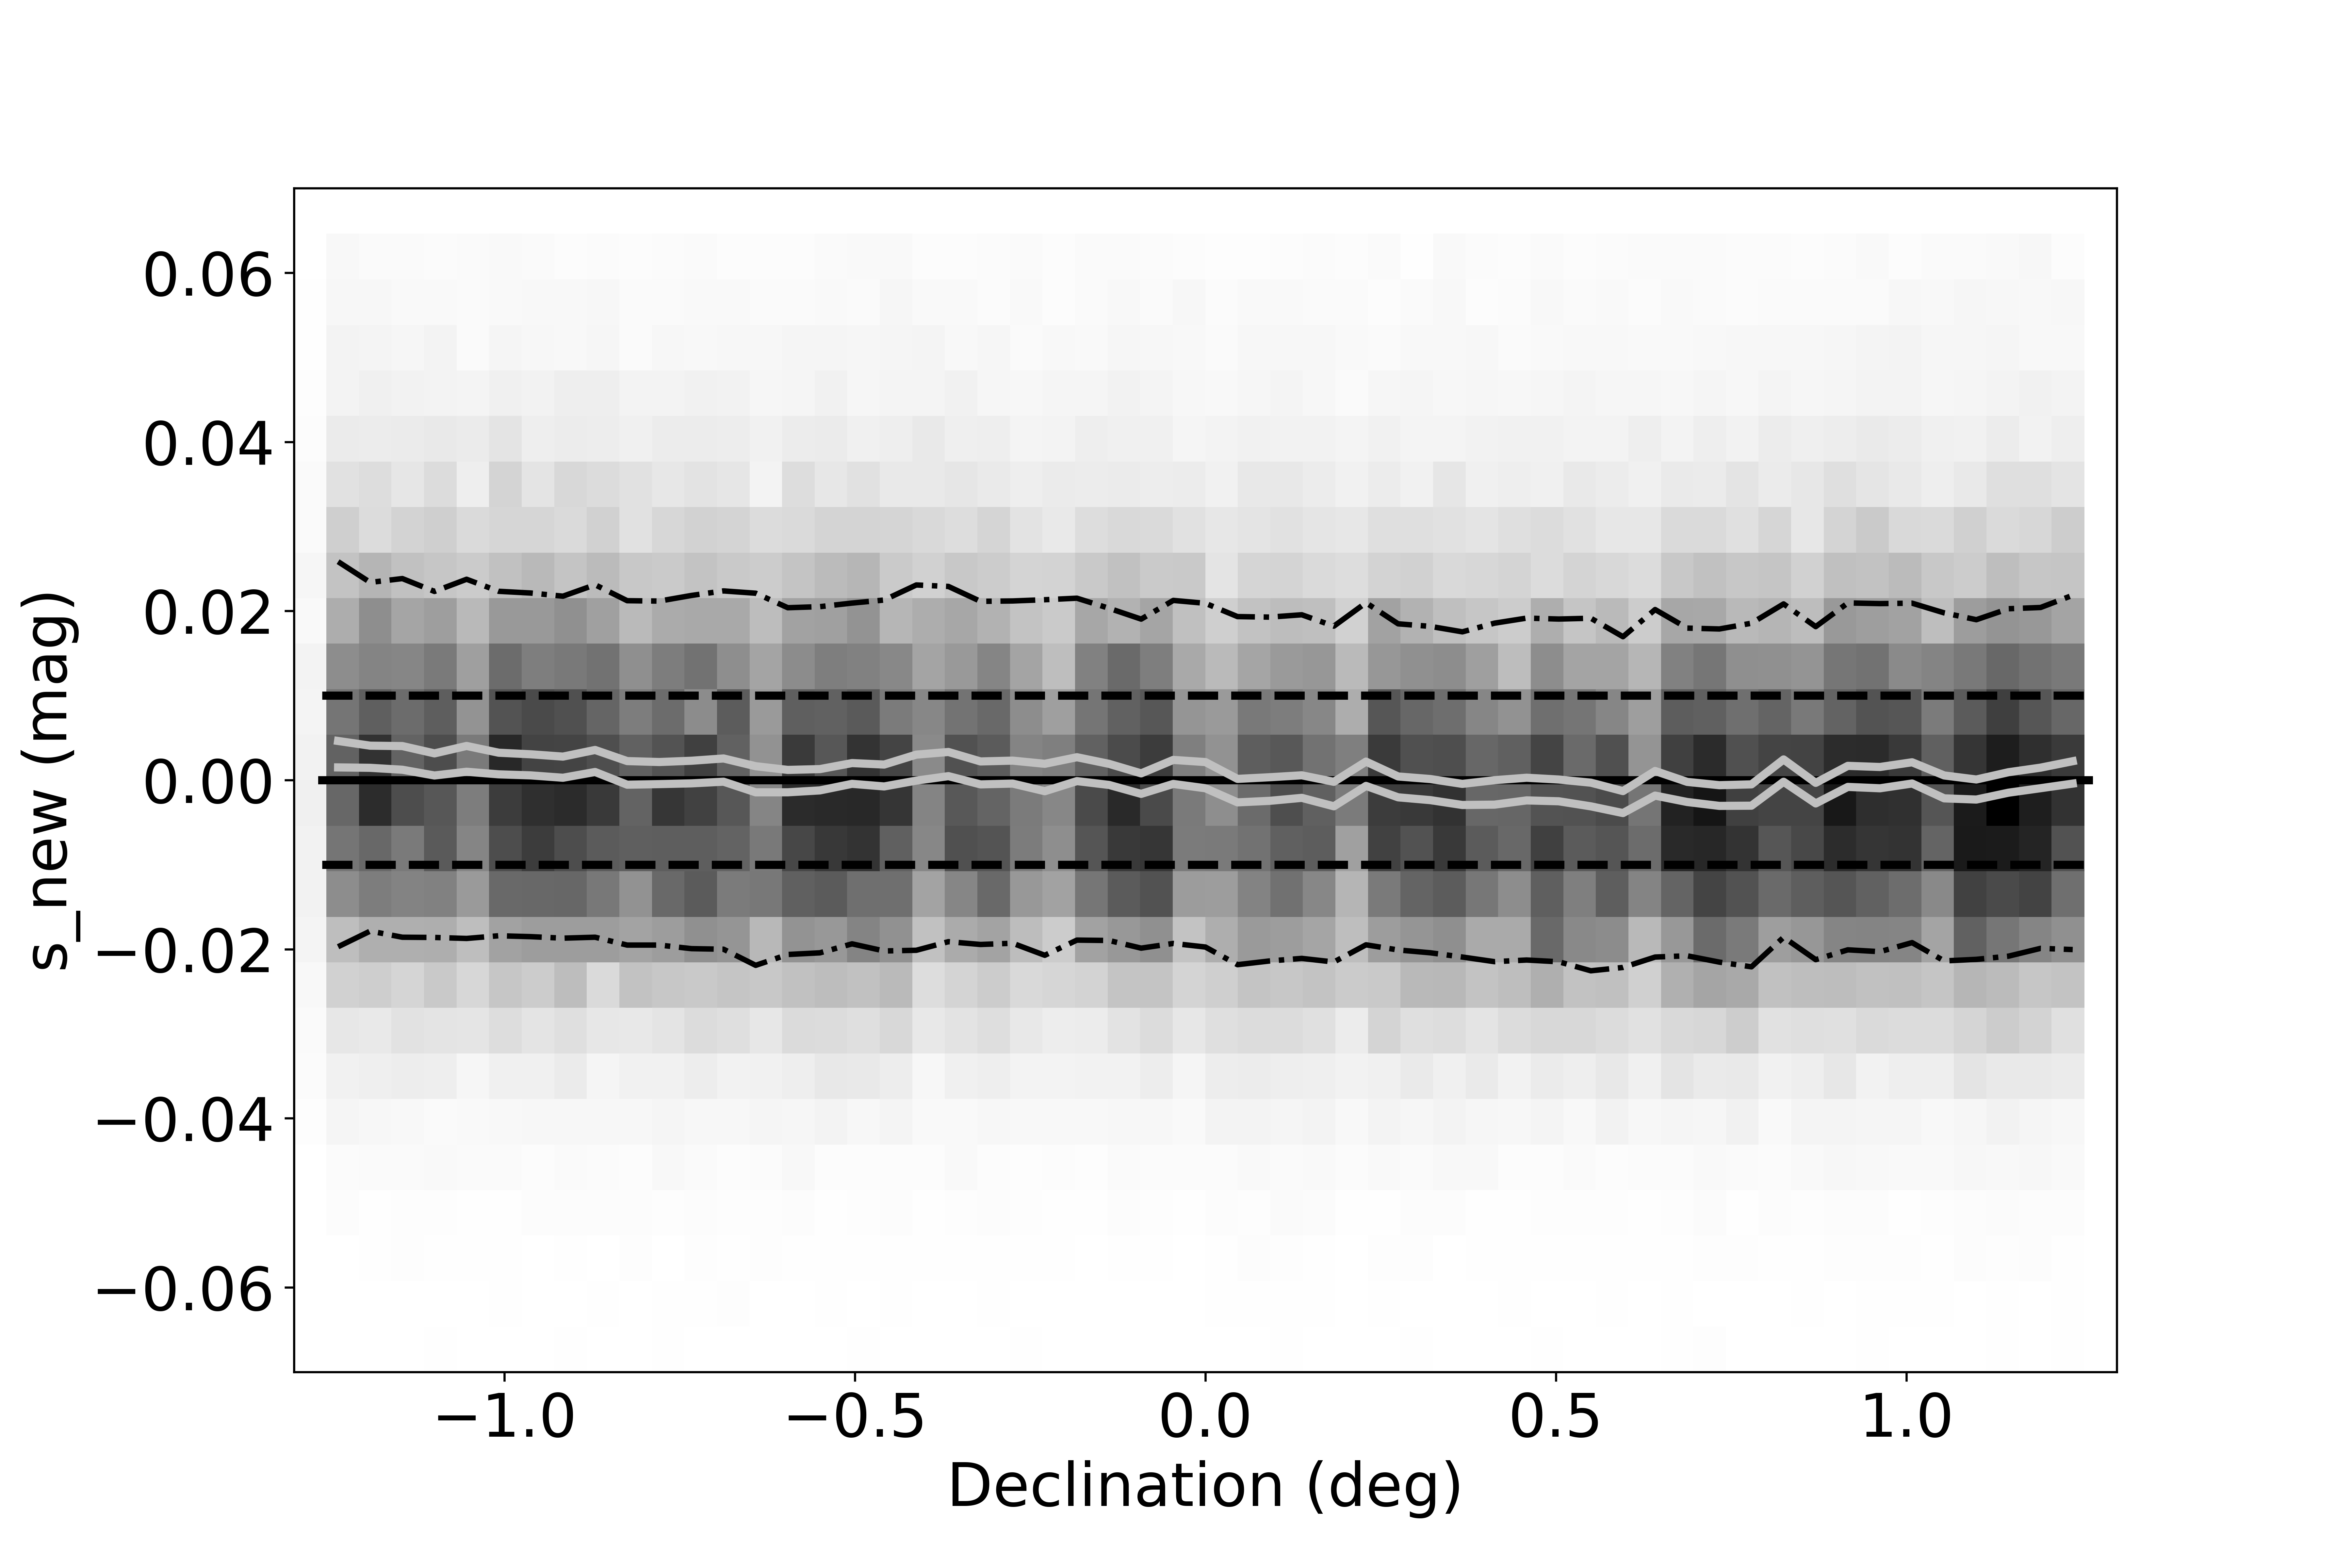
\includegraphics[width=7cm]{figures/testV26vsV33_snew_u_s_new_Dec_Hess.png} 
    \centering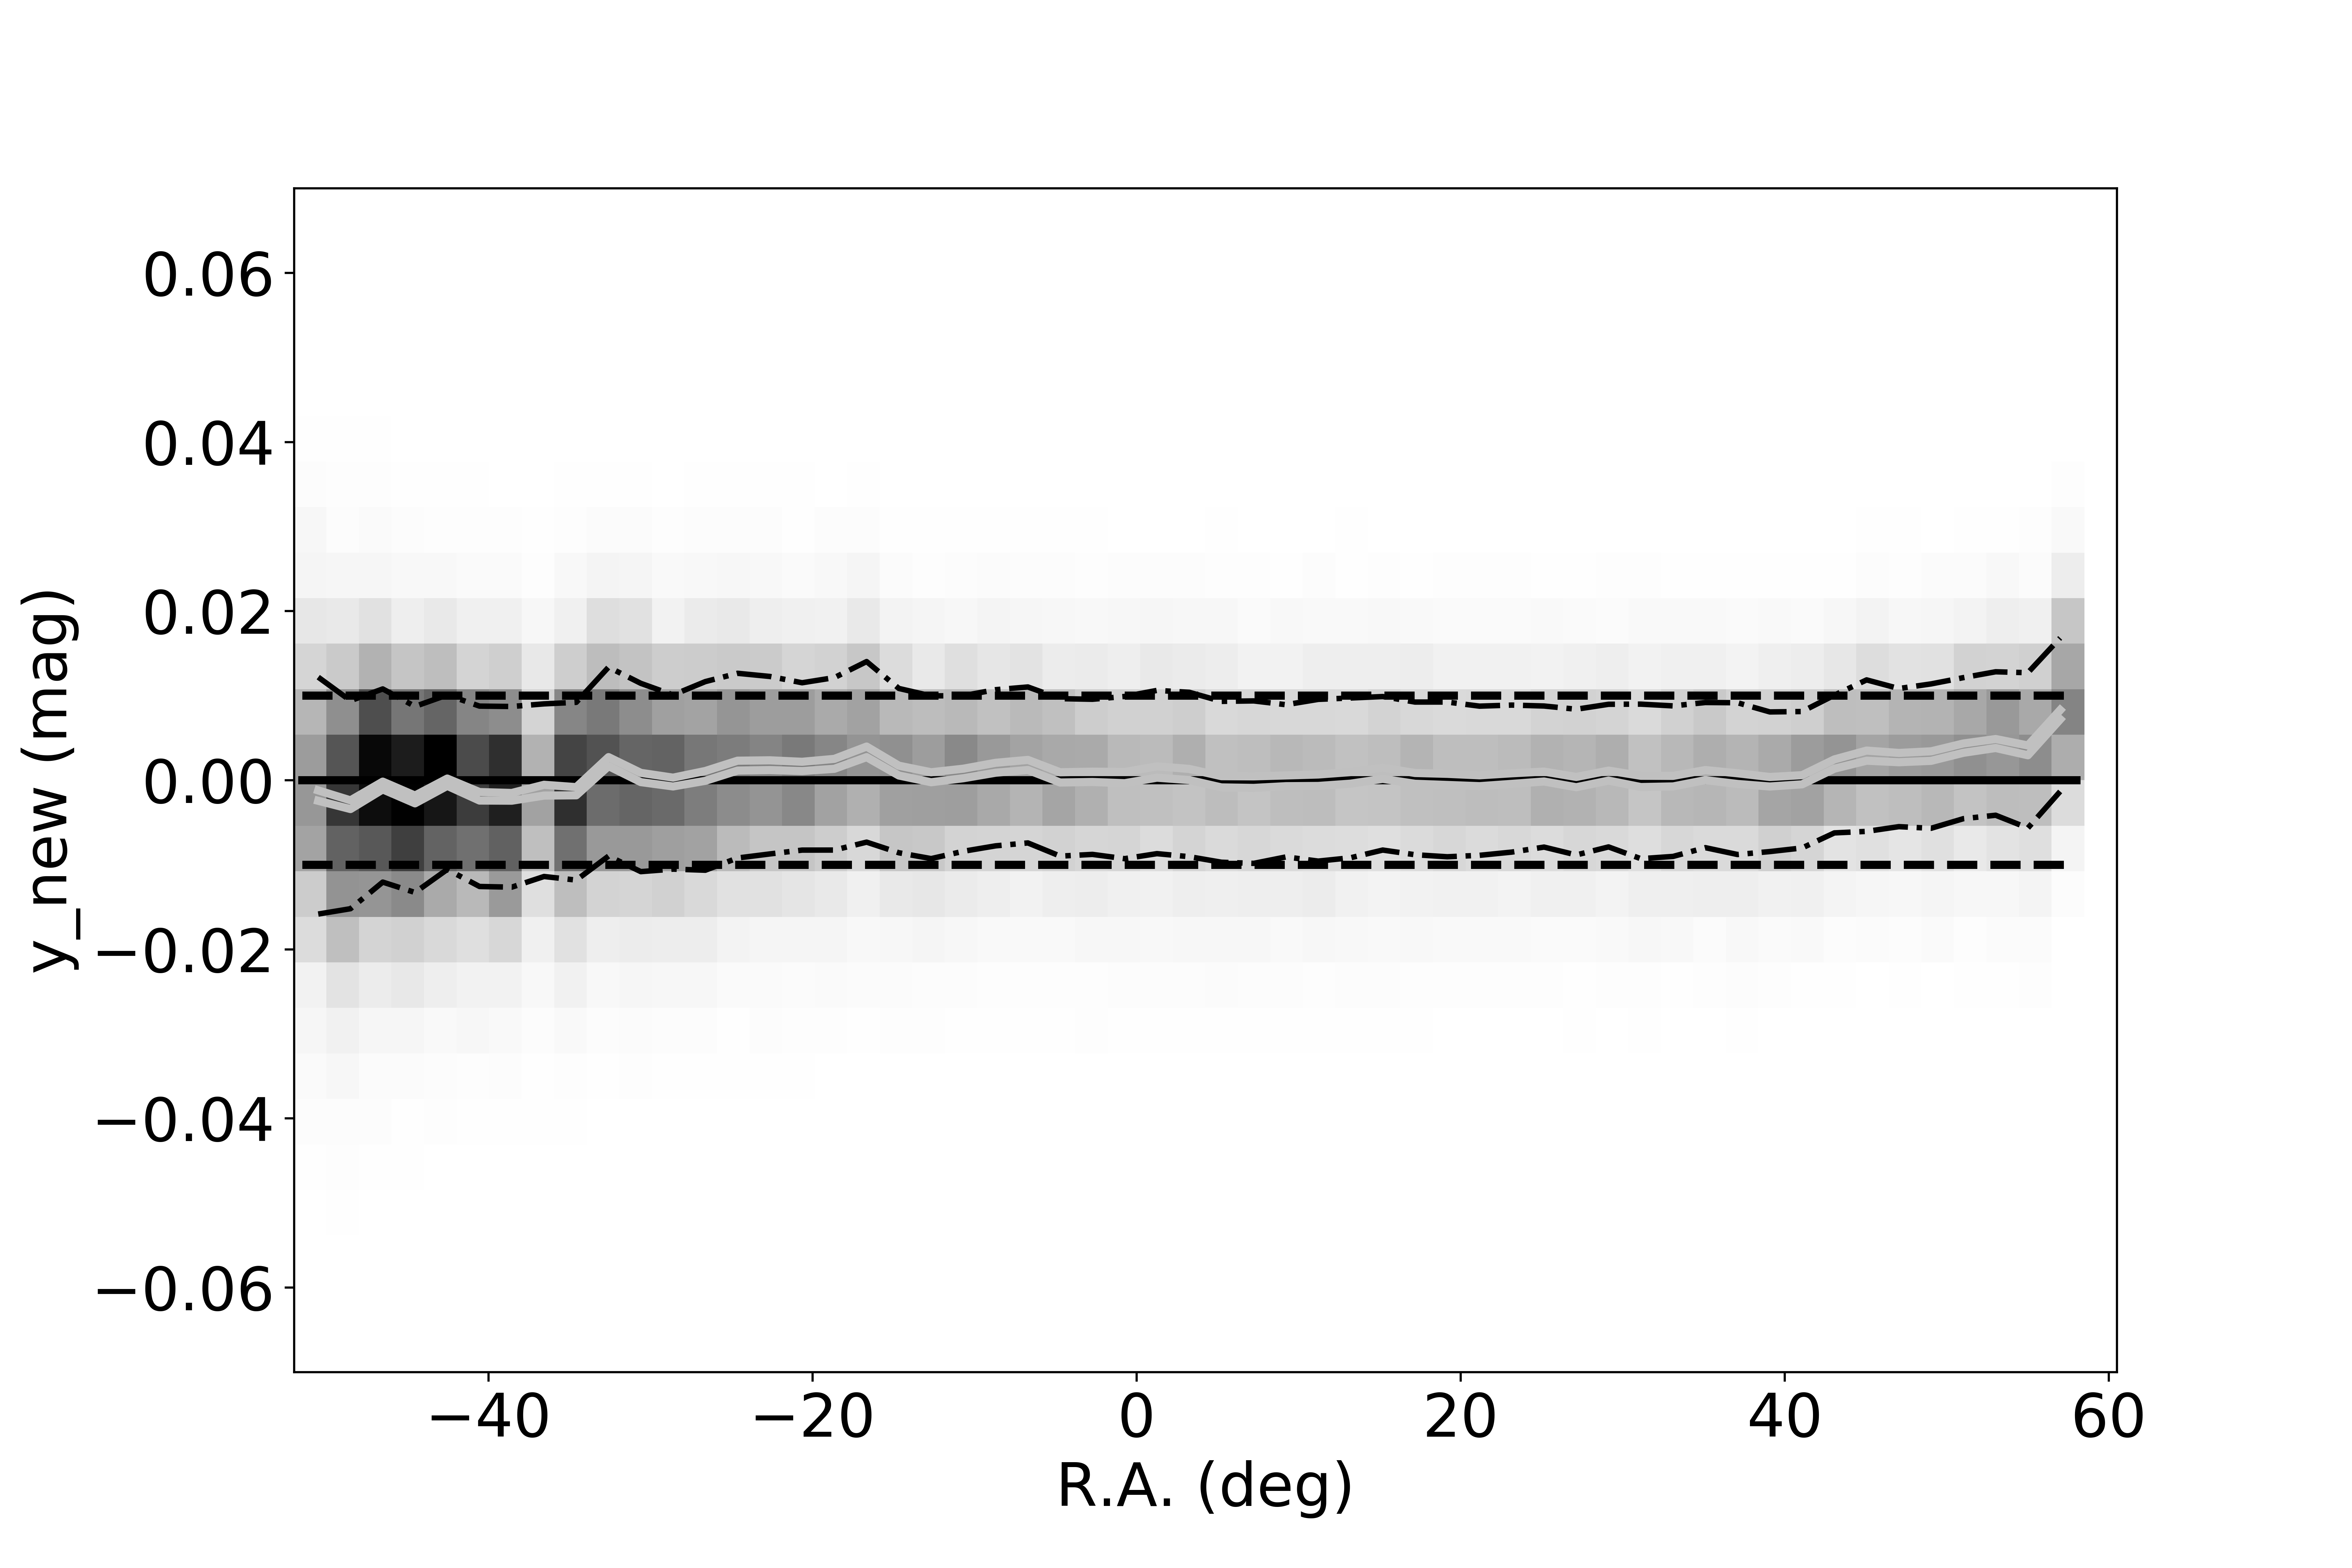
\includegraphics[width=7cm]{figures/testV26vsV33_ynew_z_y_new_RA_Hess.png} 
    \centering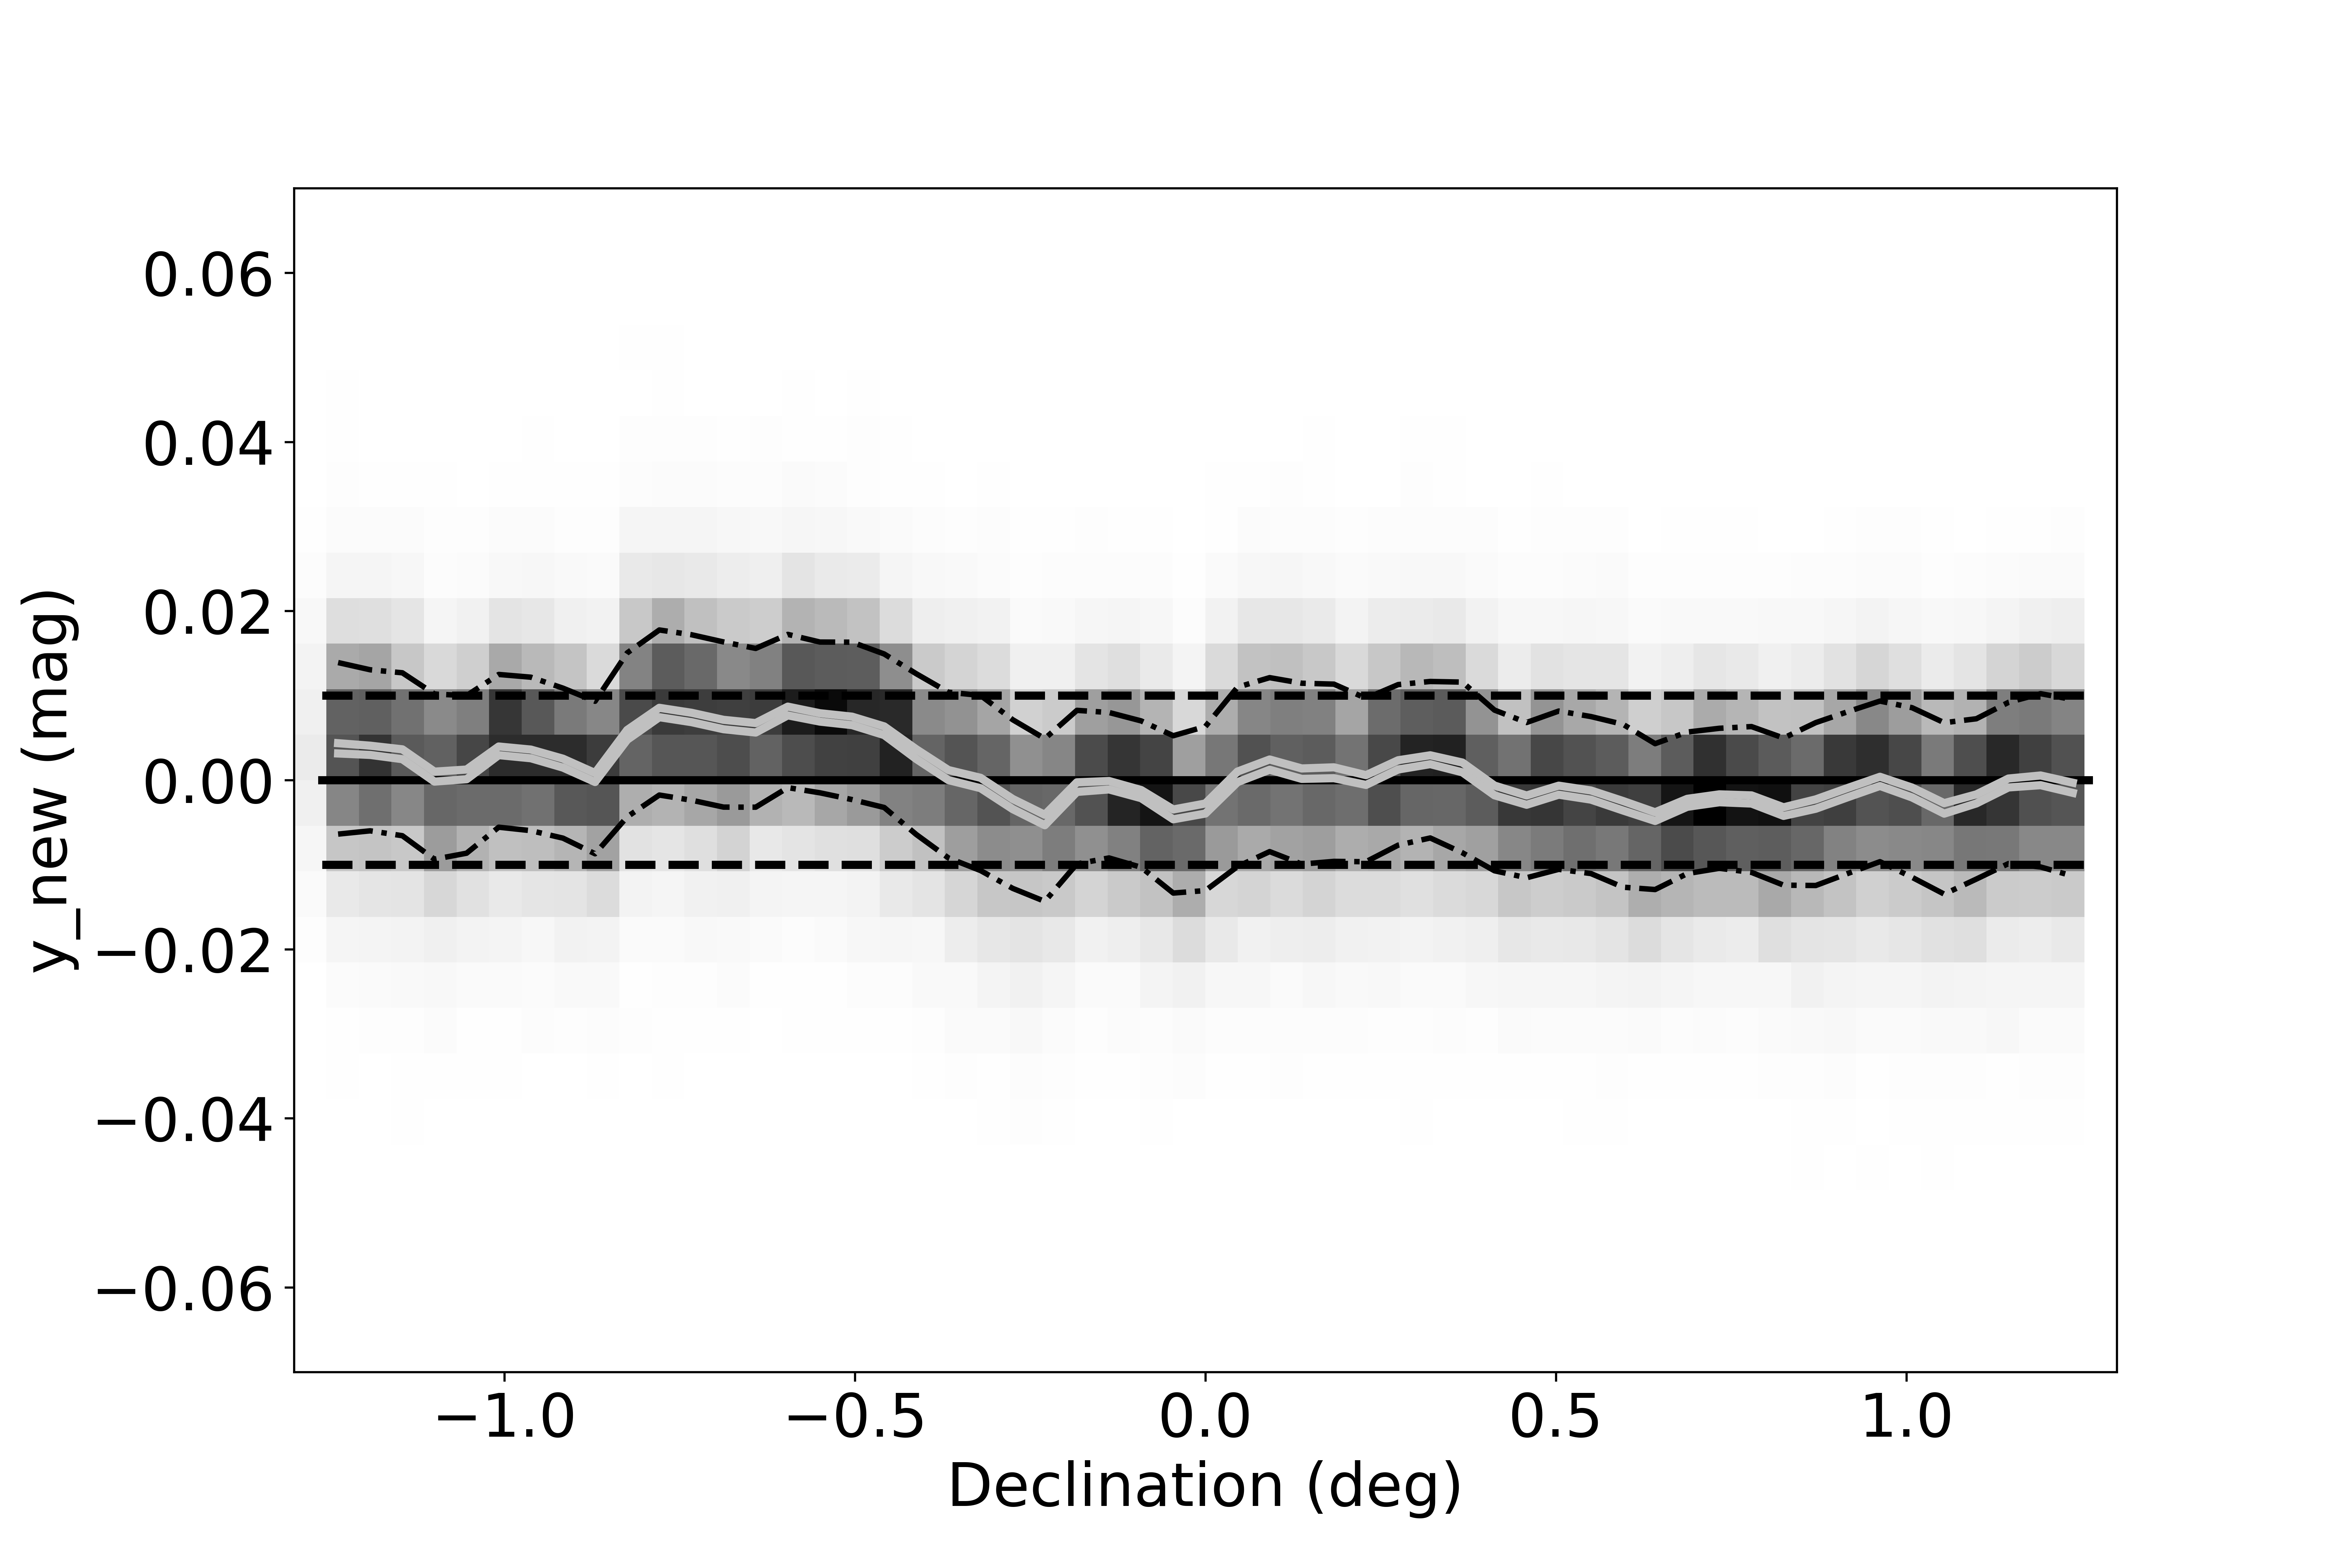
\includegraphics[width=7cm]{figures/testV26vsV33_ynew_z_y_new_Dec_Hess.png}  
\caption{The behavior of the $s$ color (top two panels), the second principal color in the SDSS
$g-r$ vs. $u-g$ color-color diagram, and the $y$ color (bottom two panels), the second 
principal color in the SDSS $i-z$ vs. $r-i$ color-color diagram, for the new v3.4 catalog.
The standard deviation of the median $s$ values binned by R.A. and Declination is 9.8 millimag 
and 1.3 millimag, respectively, and 1.8 millimag and 3.4 millimag for the $y$ color.}
\label{fig:comparesy} 
\end{figure}
  
 

\subsection{Comparison of the new v3.4 SDSS catalog and Gaia DR2 catalog \label{sec:SSCvsGaia}} 
  

\begin{figure}
    \centering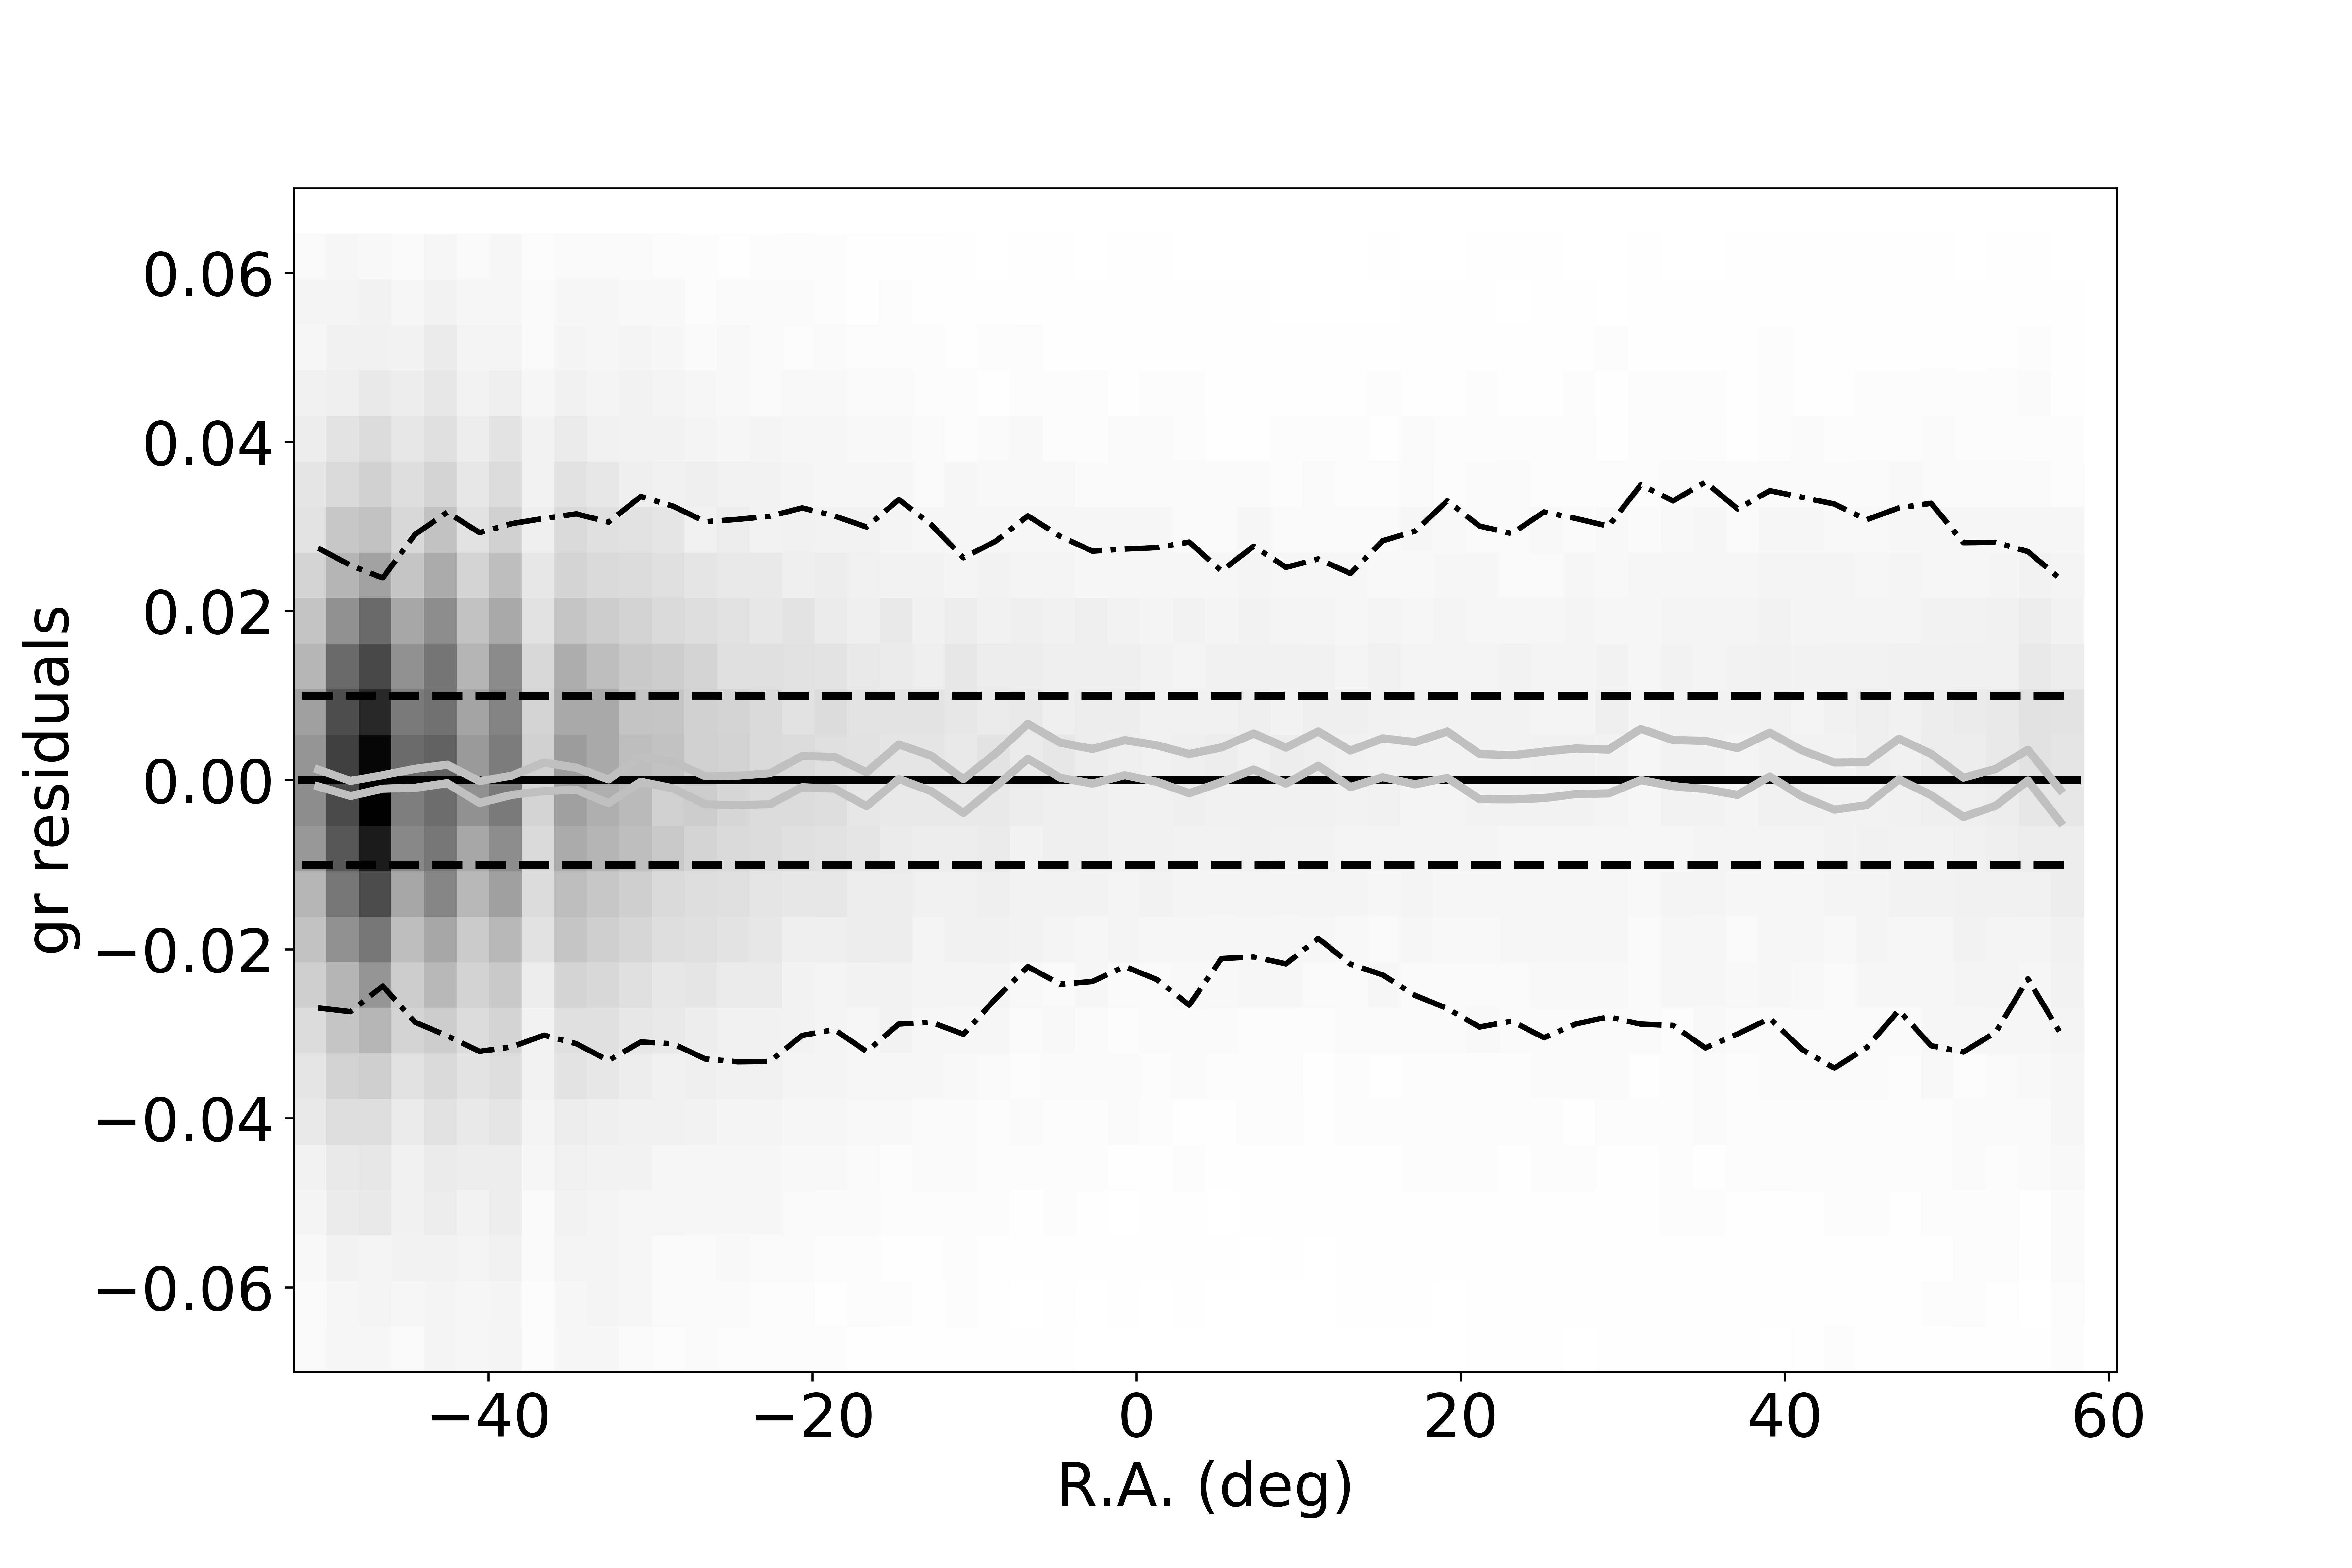
\includegraphics[width=7cm]{figures/colorResidGaiaColors_gr_RA_Hess.png} 
    \centering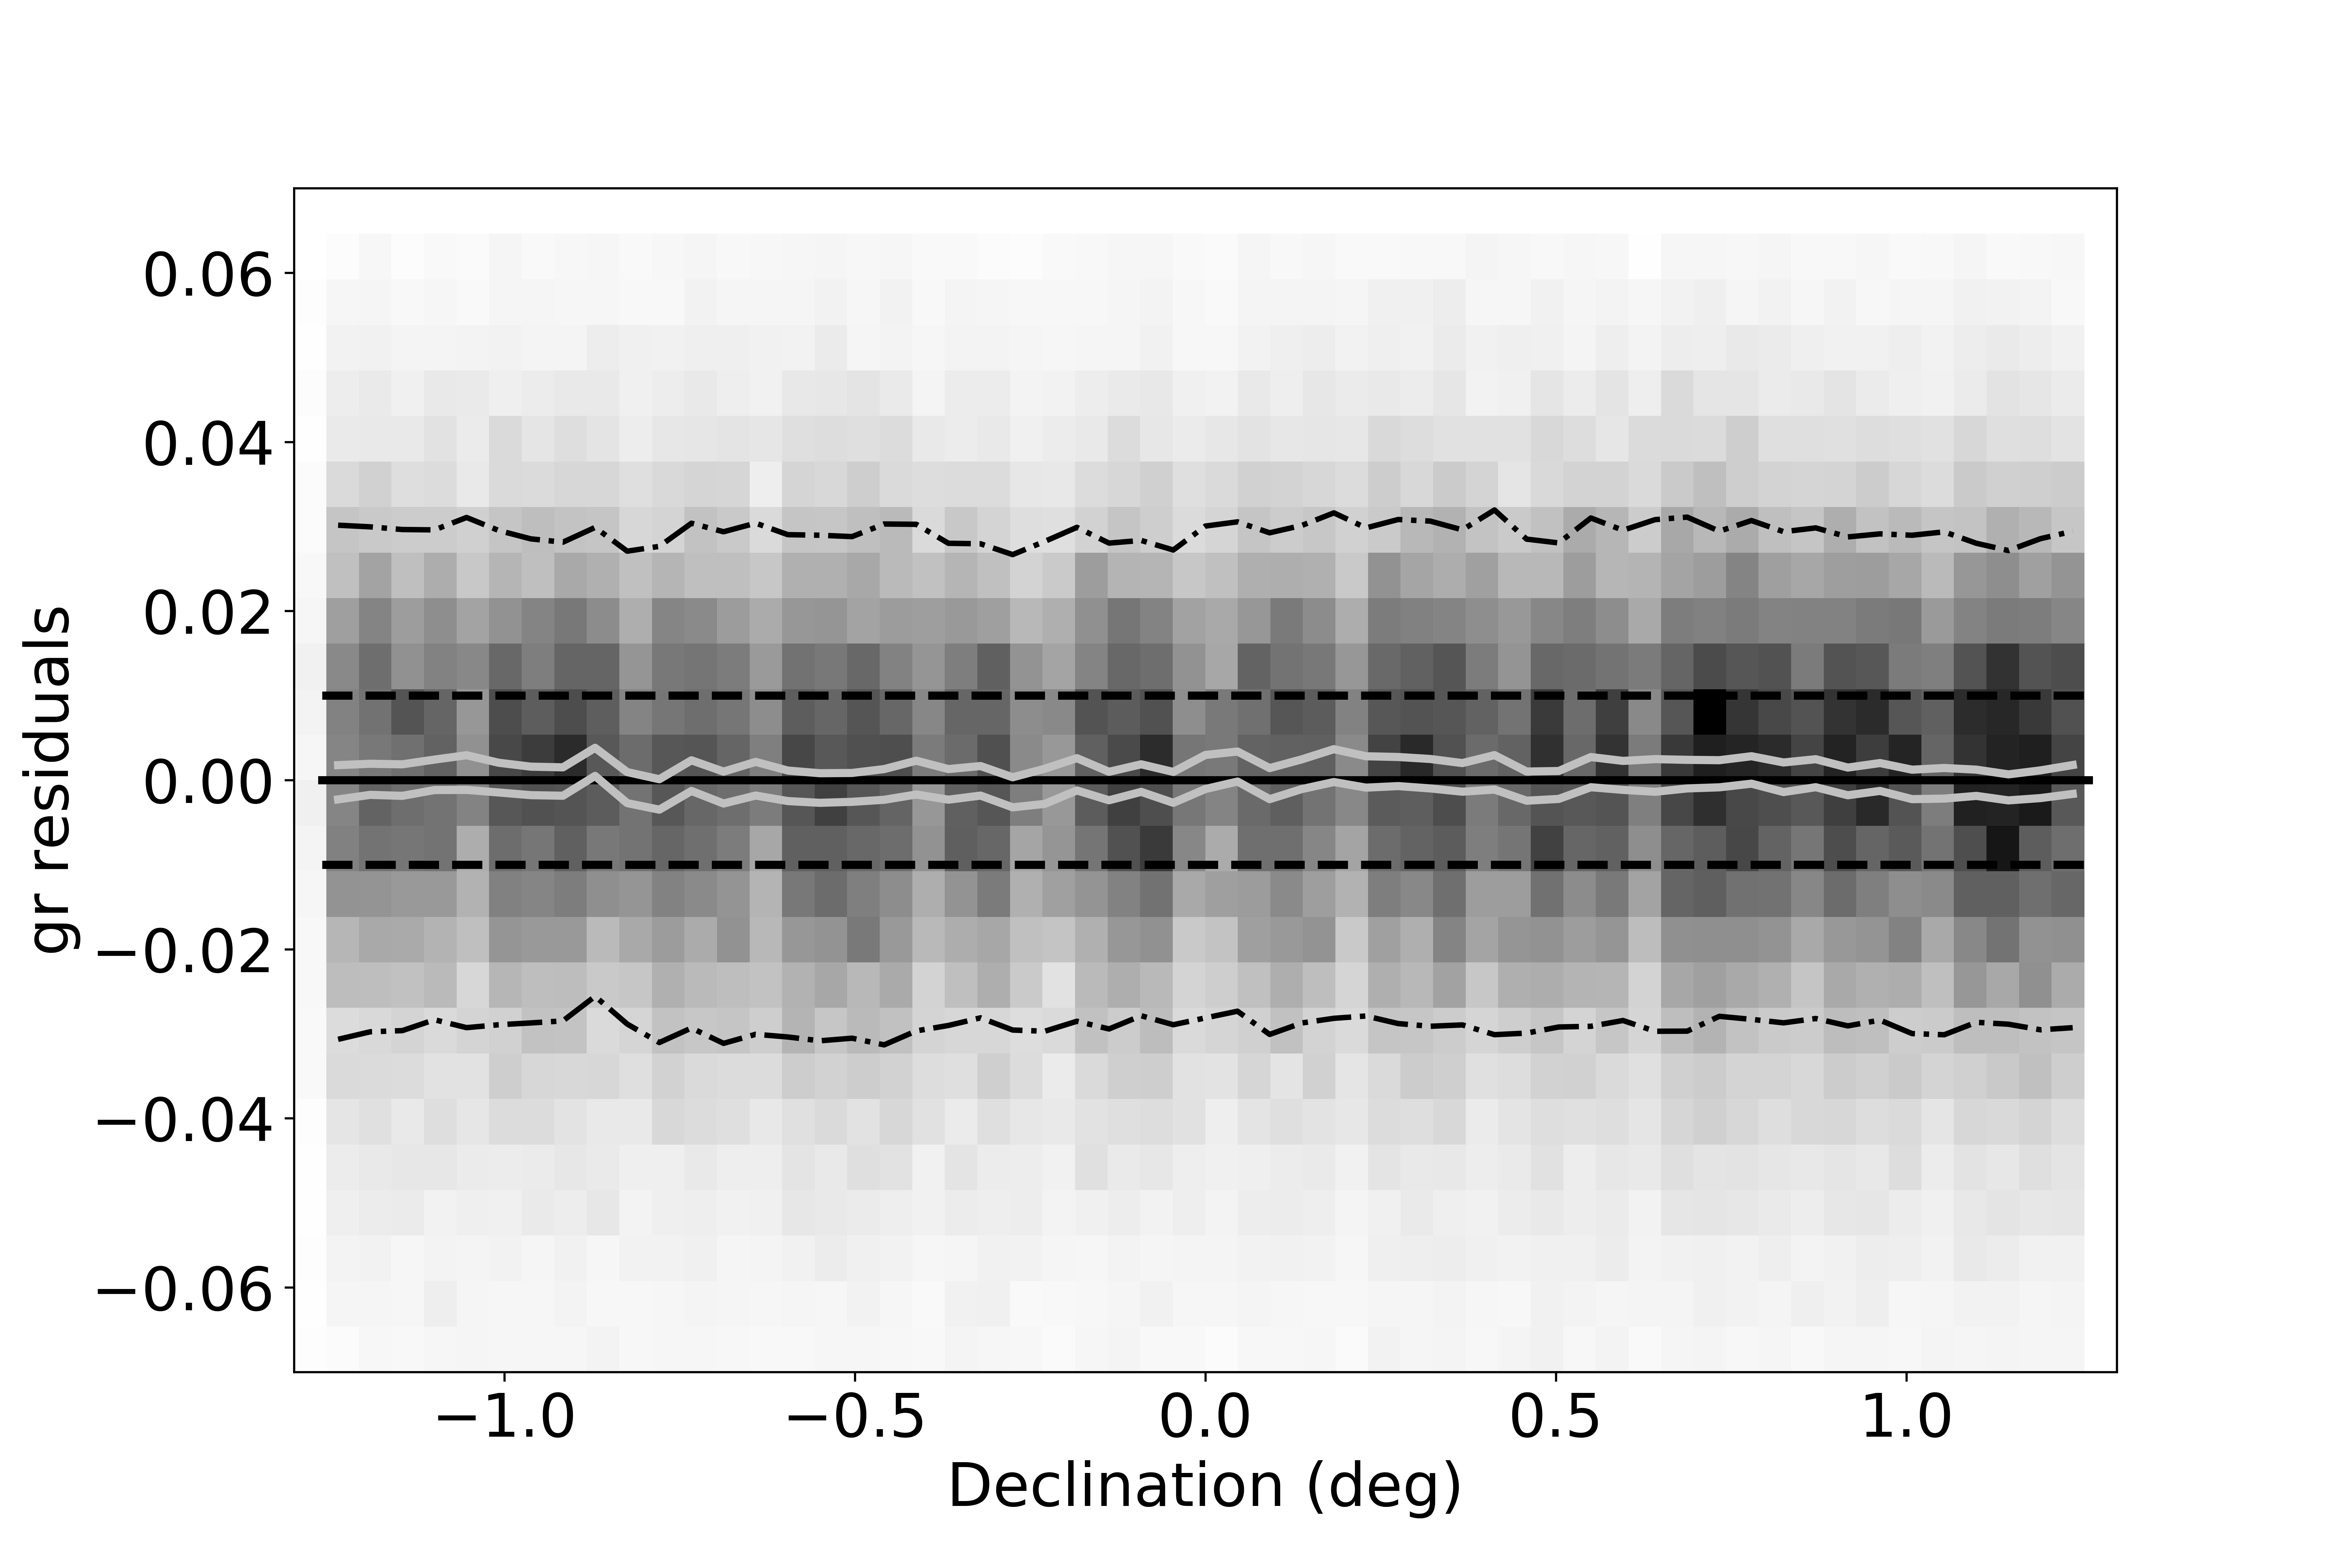
\includegraphics[width=7cm]{figures/colorResidGaiaColors_gr_Dec_Hess.png} 
\caption{Left: analogous to Figure~\ref{fig:graycorrRA}, except that here residuals between
the SDSS $g-r$ color from the v3.4 catalog and a synthetic $g-r$ color generated using 
Gaia's $BP-RP$ color are shown. The binned median scatter is 1.6 millimag. Right: the 
$g-r$ residuals are shown as a function of Declination. The binned median scatter is 0.8 millimag.
}
\label{fig:grVSgaiaRADec}
\end{figure}
 

\subsection{Comparison of the new v3.4 SDSS catalog with DES and Pan-STARRS catalogs \label{sec:DESPS1}} 
  
 
Conclusion: in RA: 3-7 millimag, Dec: 1-2 millimag  (CFIS: 6 millimag in u) 


\begin{deluxetable}{l|c|c|c|c}[ht!]
\tablecaption{The robust standard deviation for binned median magnitude differences between
the new v3.4 SDSS catalog, and DES and Pan-STARRS1 (PS1) catalogs (millimag). \label{tab:DESPS1}}
\tablehead{
\colhead{Band} & \colhead{DES R.A.} & \colhead{DES Dec} & \colhead{PS1 R.A.} & \colhead{PS1 Dec} 
}
\startdata
       $g$        &        5.1    &      1.8   &        3.4    &      1.4        \\
       $r$         &        4.1    &      0.8   &        2.6    &      0.7         \\  
       $i$         &        7.3    &      1.6   &        3.2    &      1.0         \\ 
       $z$        &       13.6    &     3.6   &        6.8    &      2.3         \\ 
\enddata
\end{deluxetable}
   


\begin{figure}
    \centering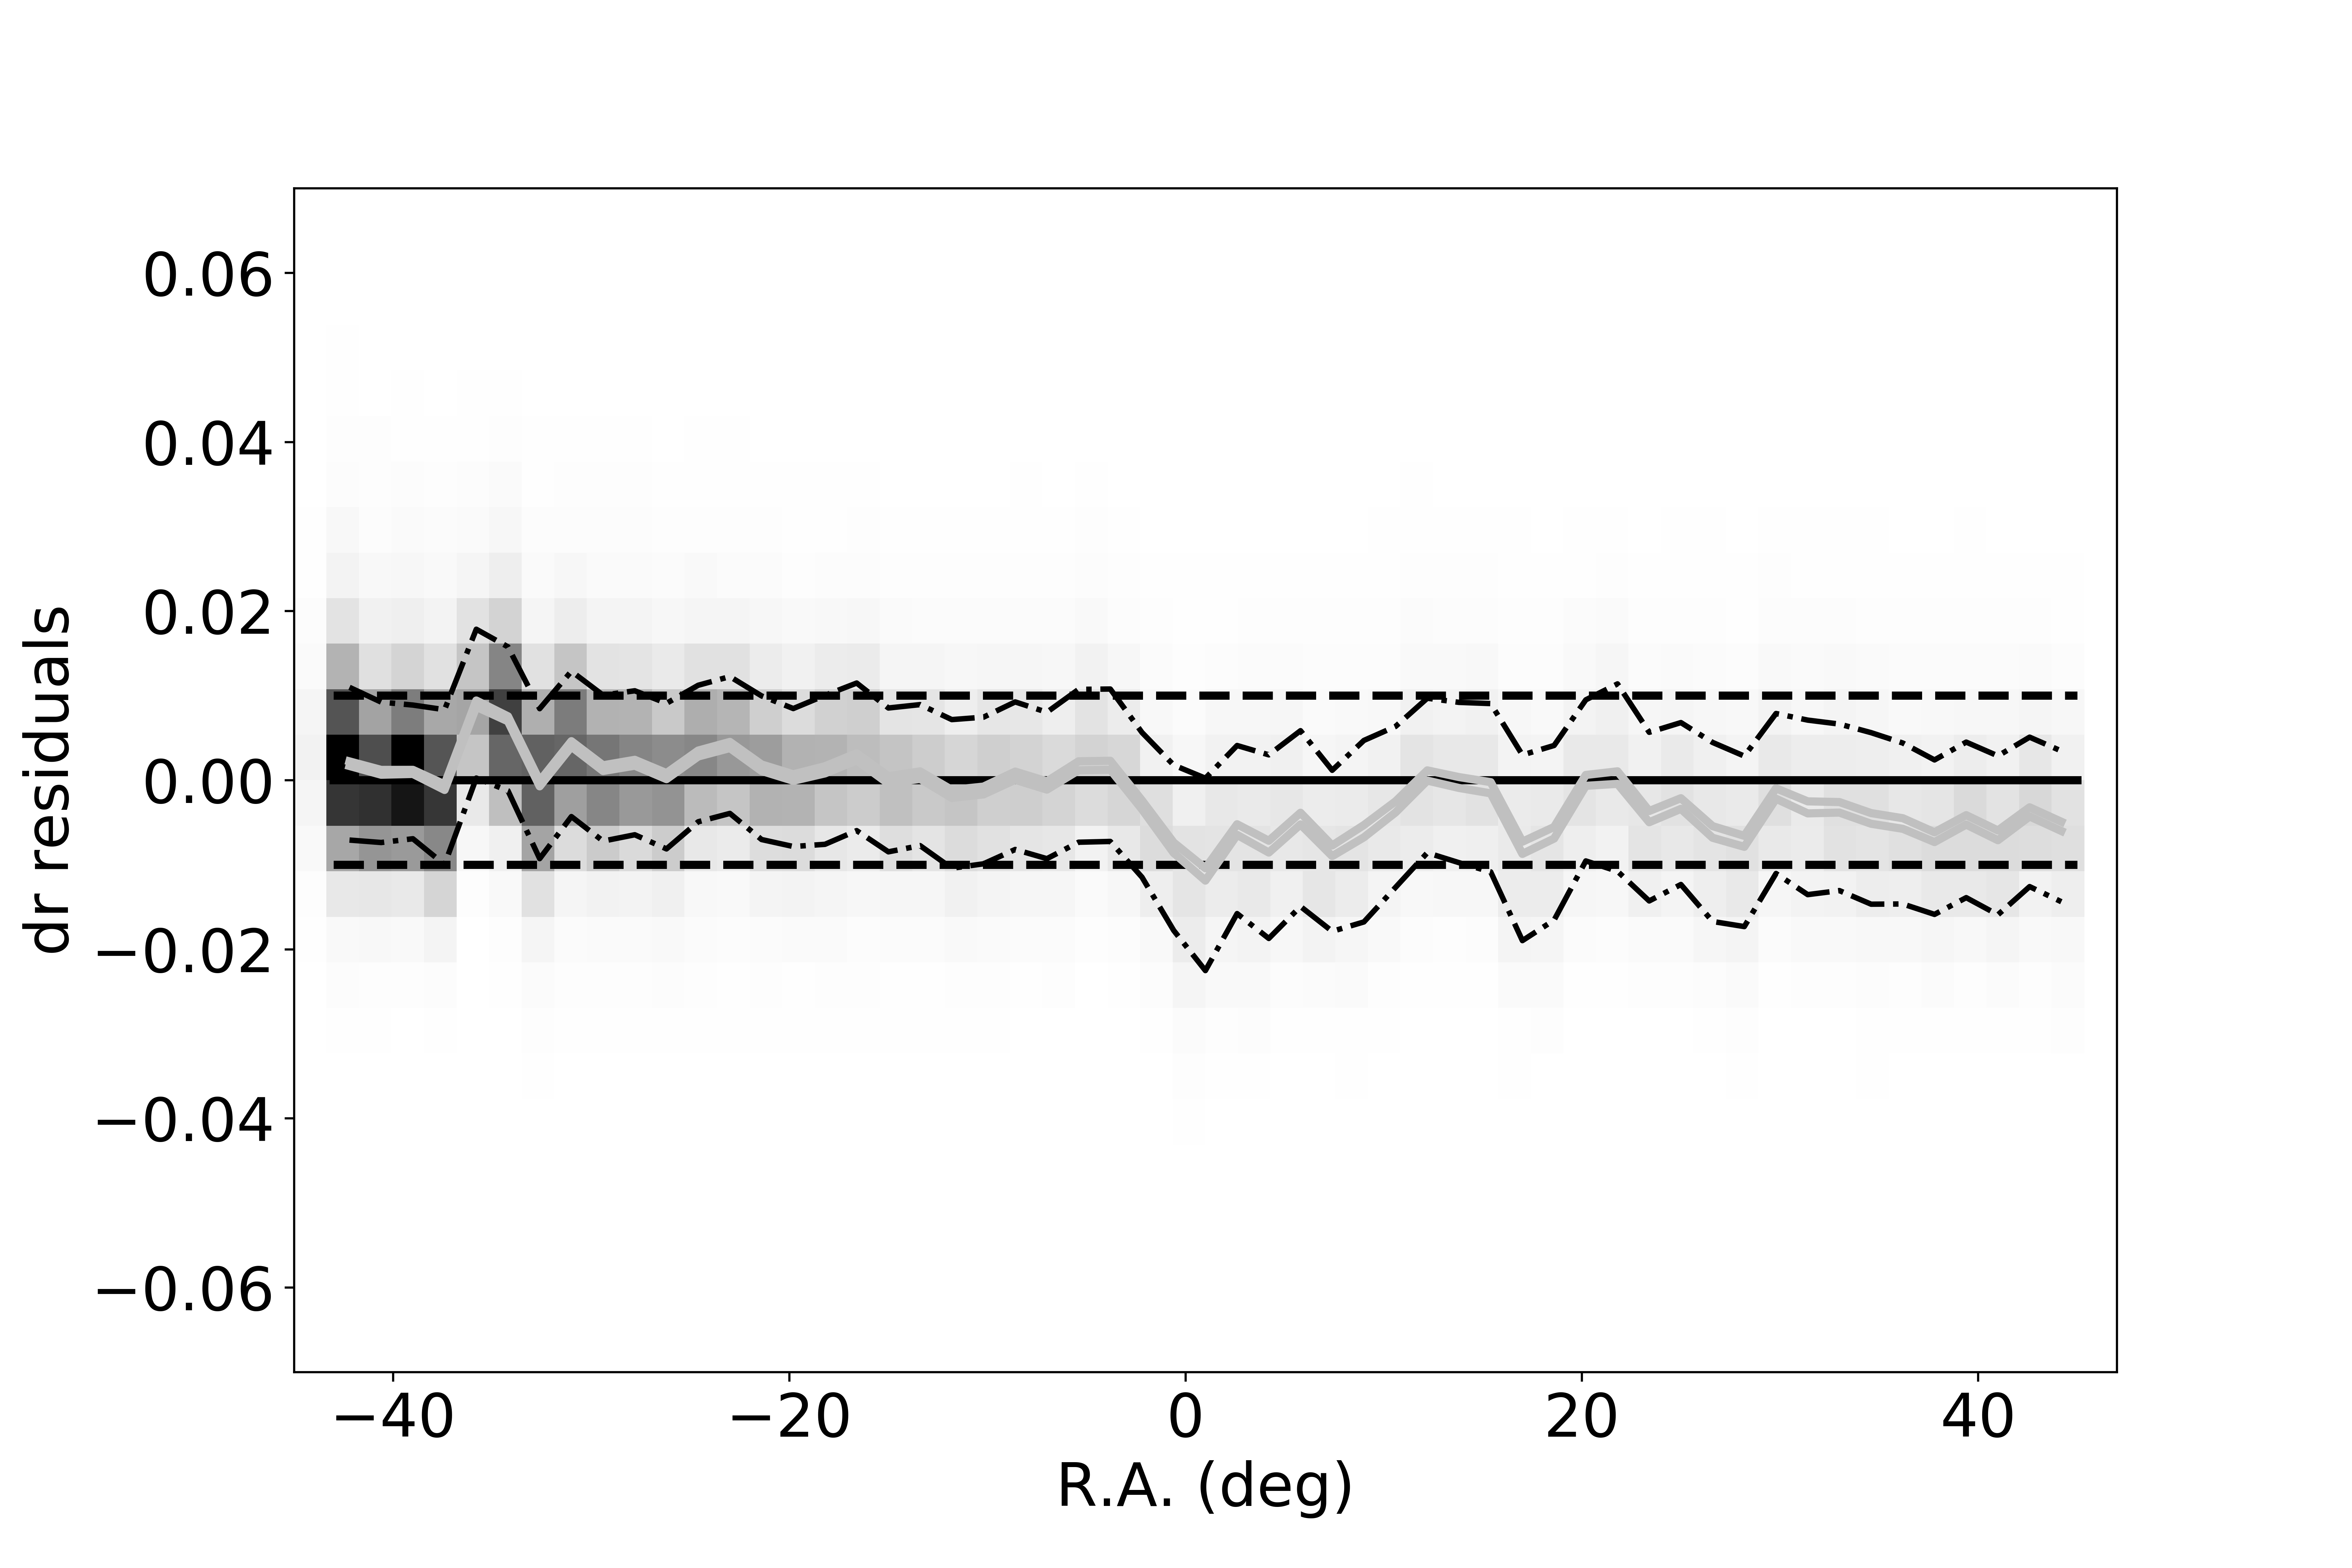
\includegraphics[width=7cm]{figures/colorResidDES2bright_dr_RA_Hess.png}
    \centering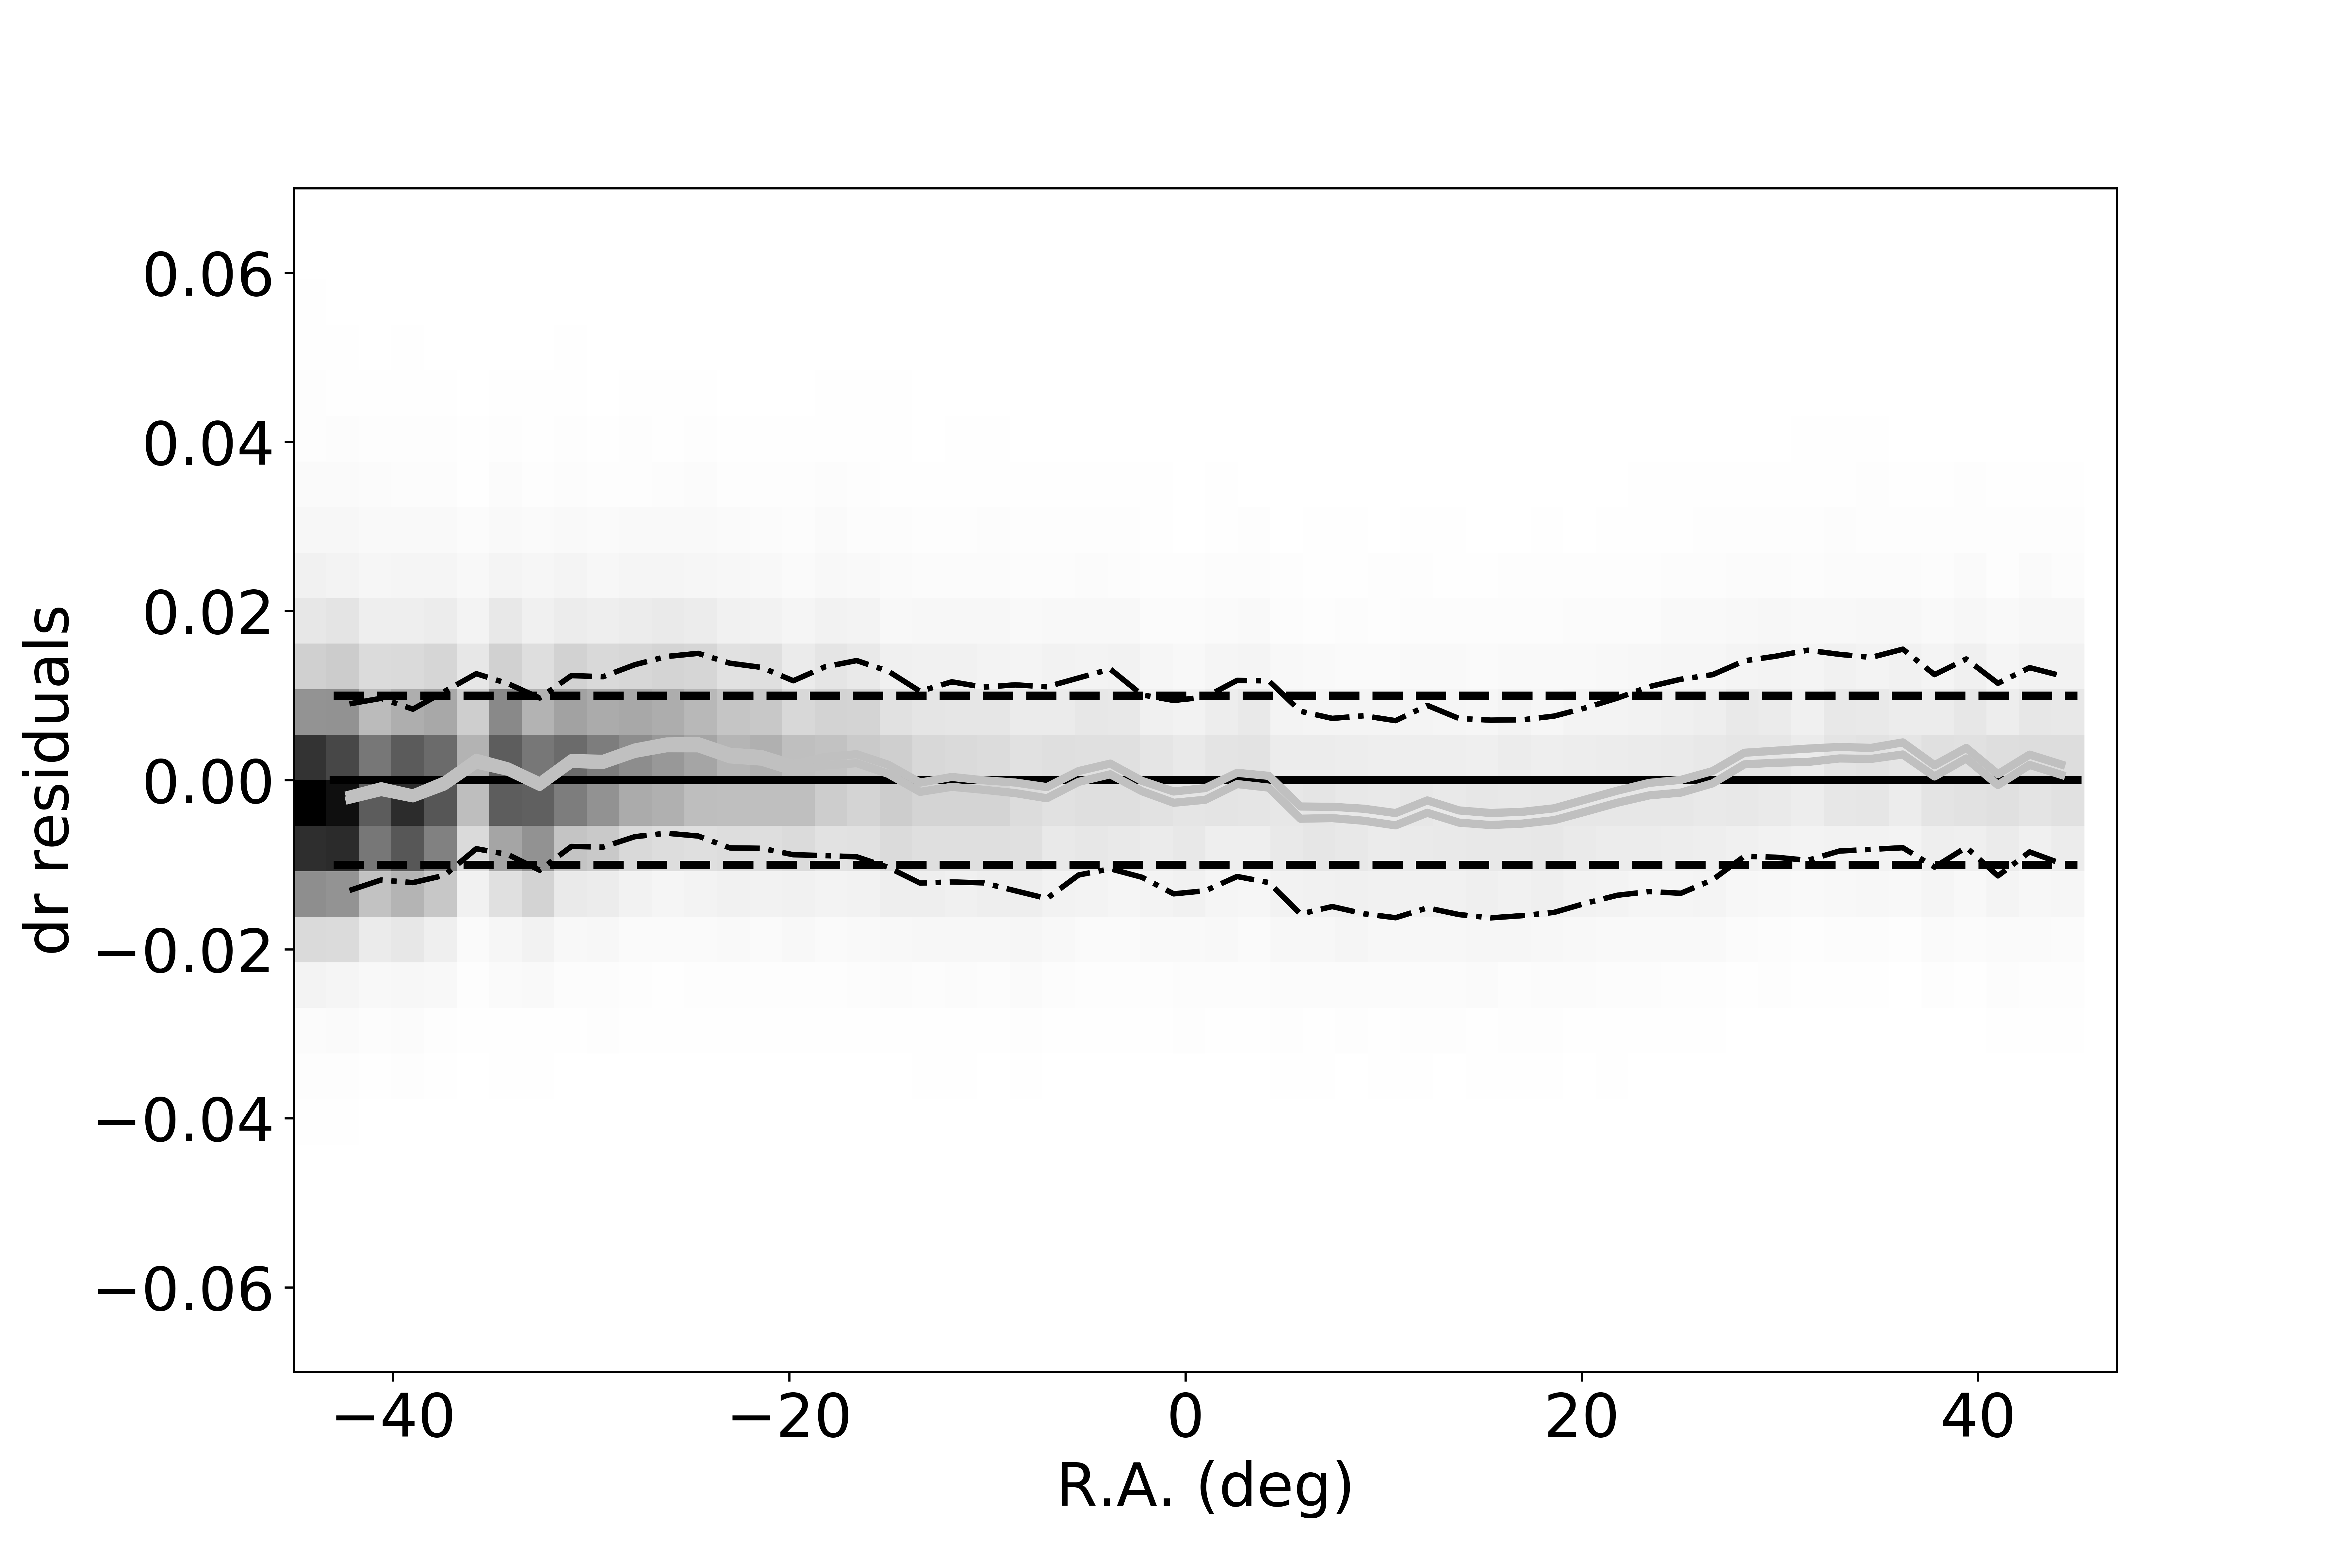
\includegraphics[width=7cm]{figures/colorResidPSbright_dr_RA_Hess.png}
    \centering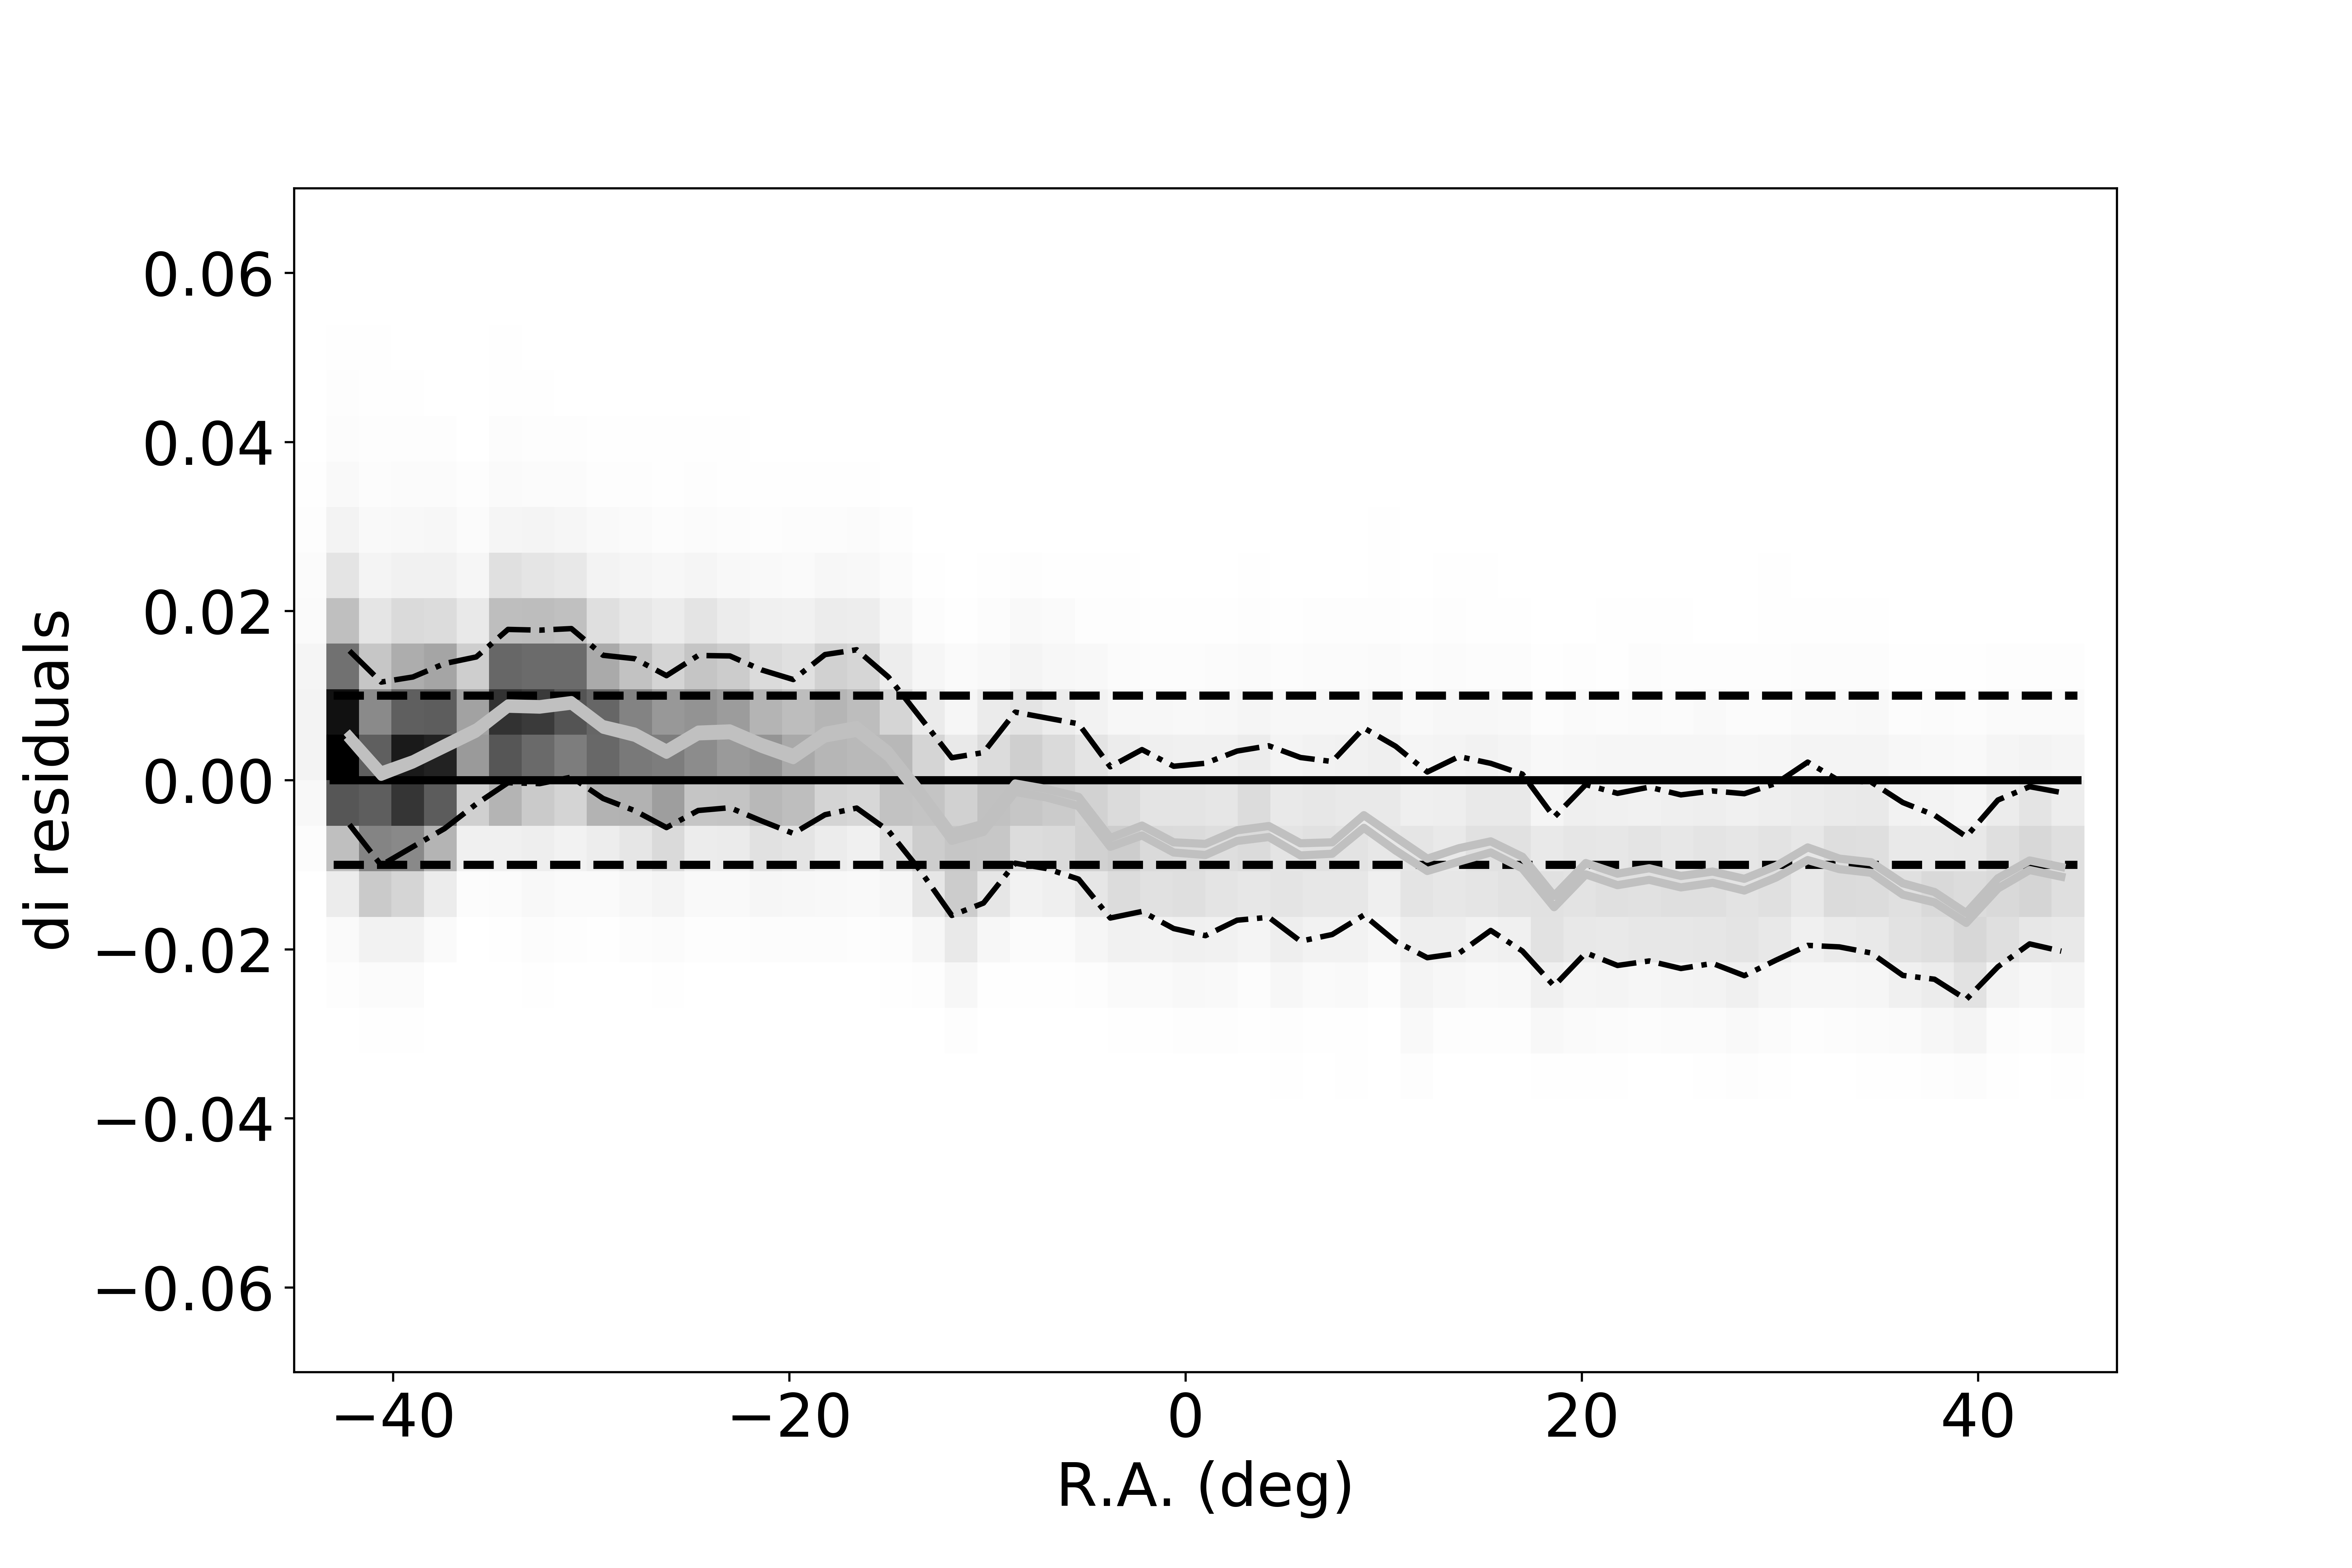
\includegraphics[width=7cm]{figures/colorResidDES2bright_di_RA_Hess.png}
    \centering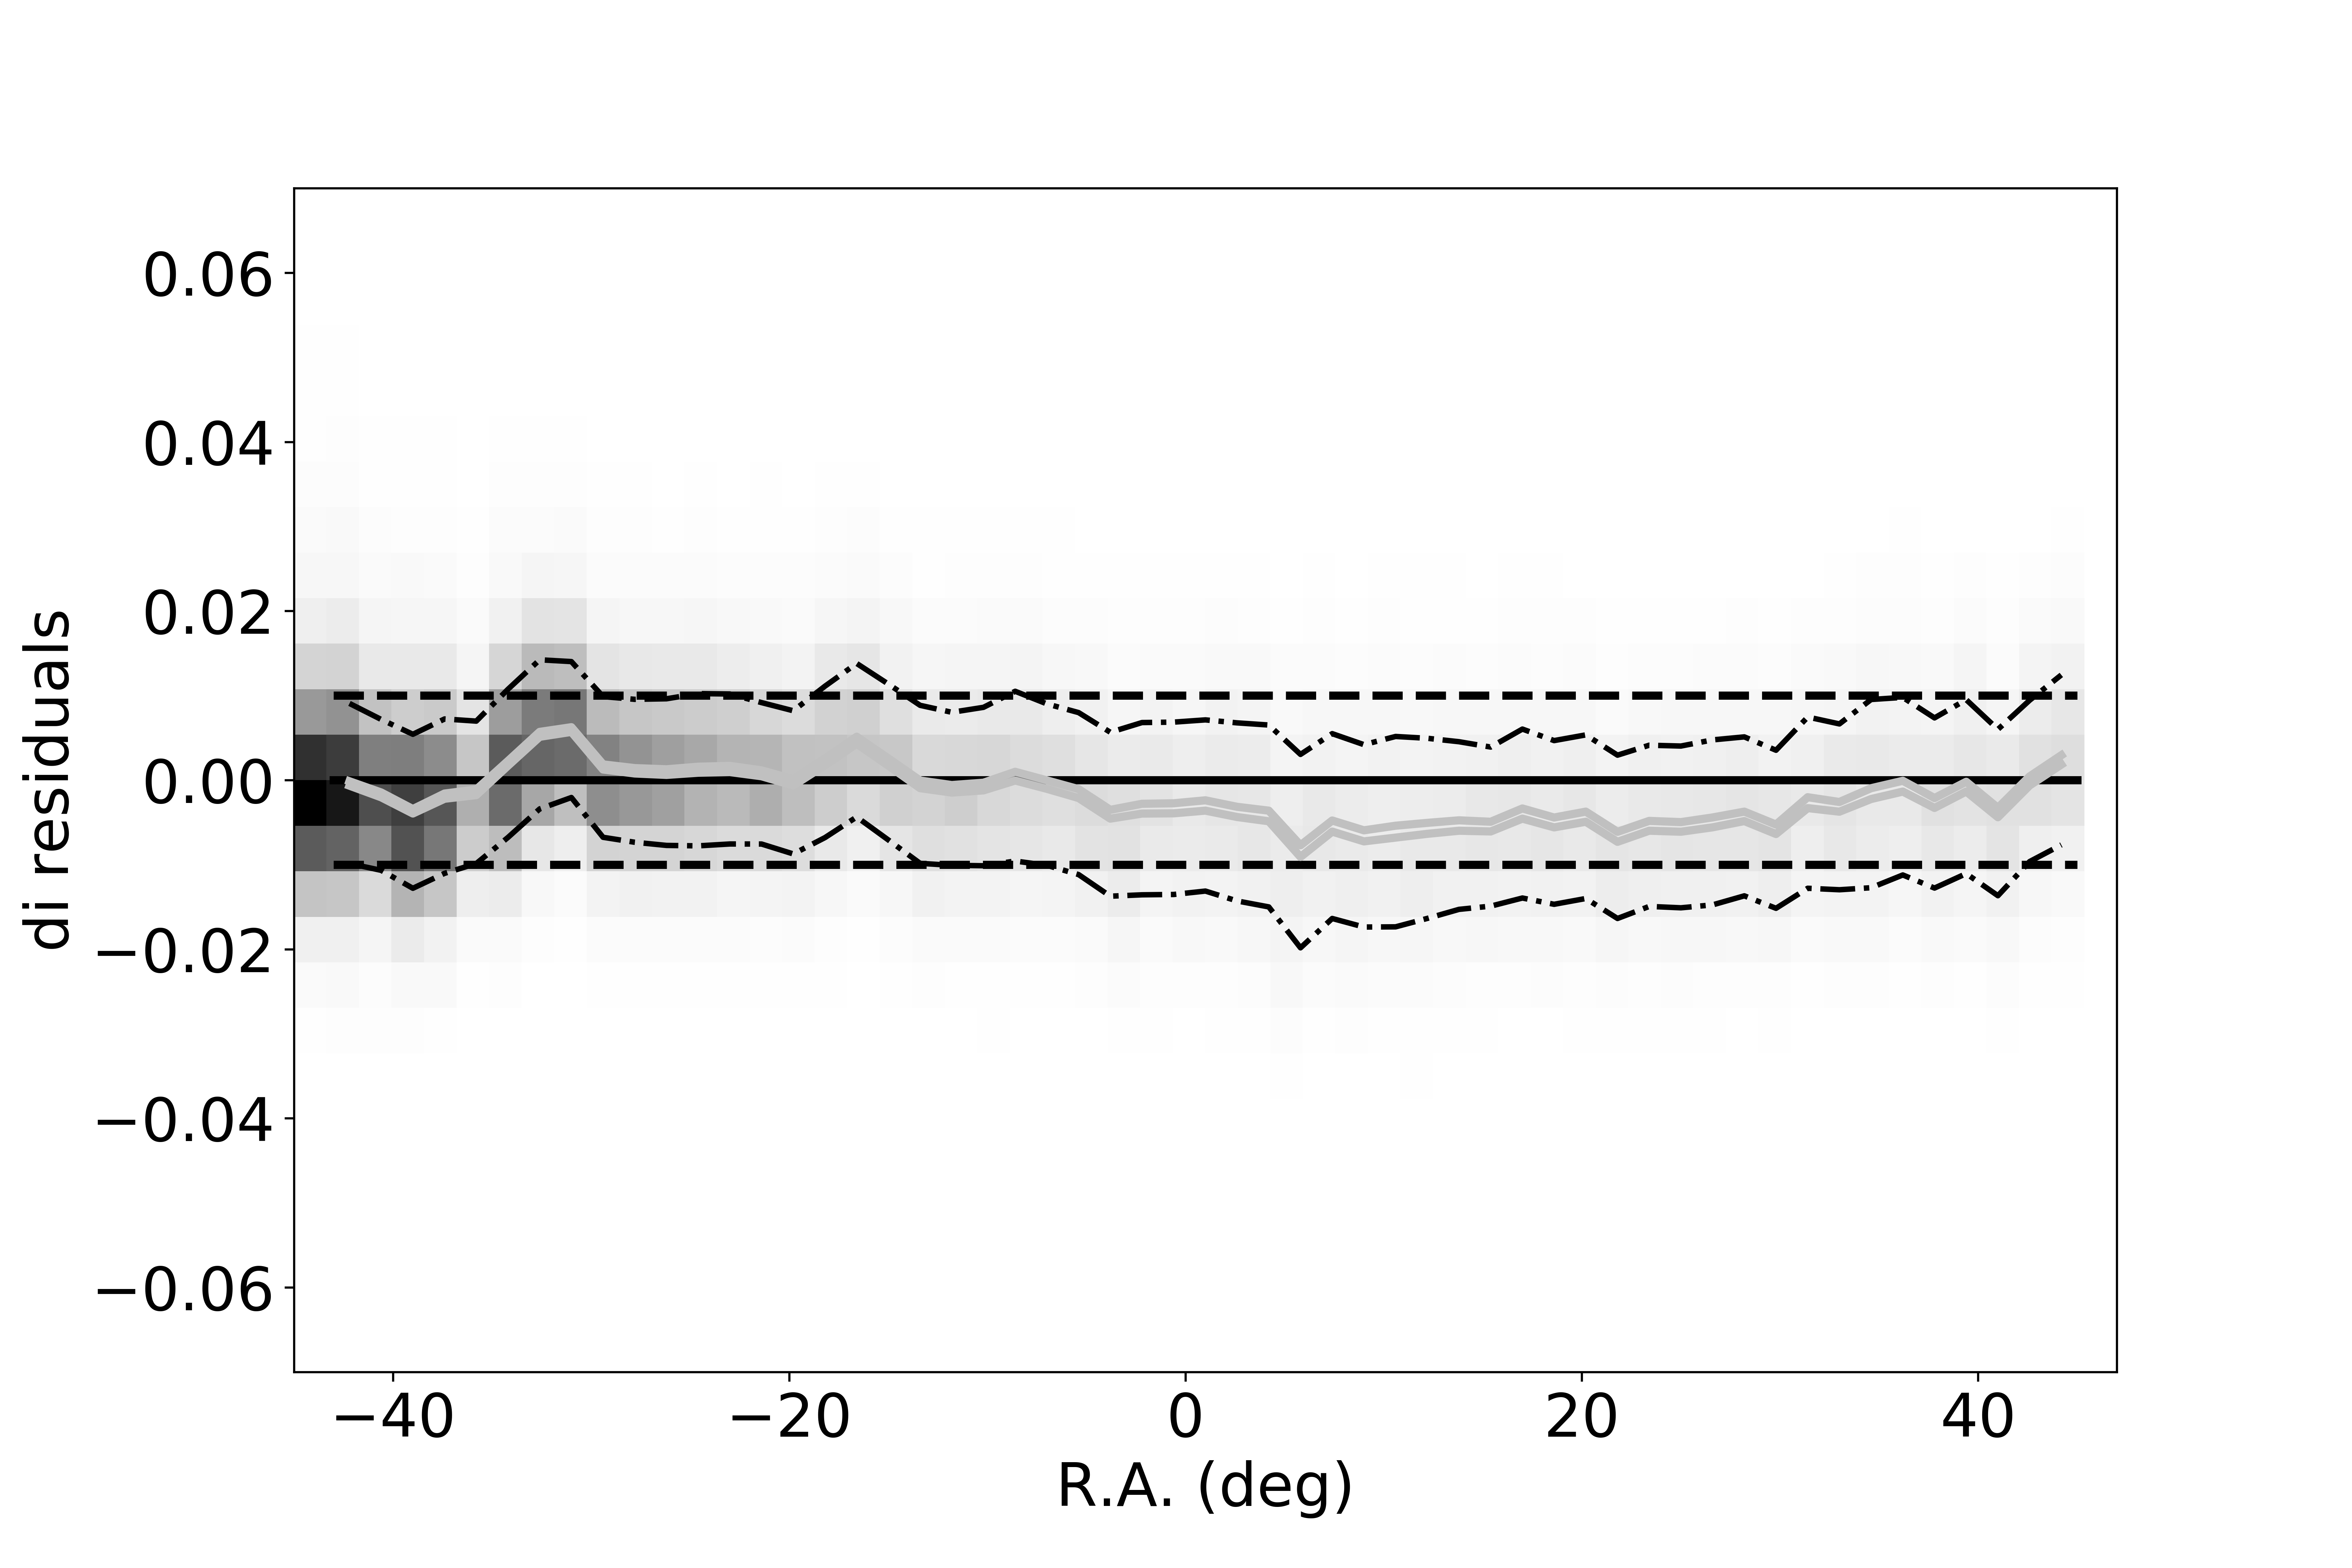
\includegraphics[width=7cm]{figures/colorResidPSbright_di_RA_Hess.png}
    \centering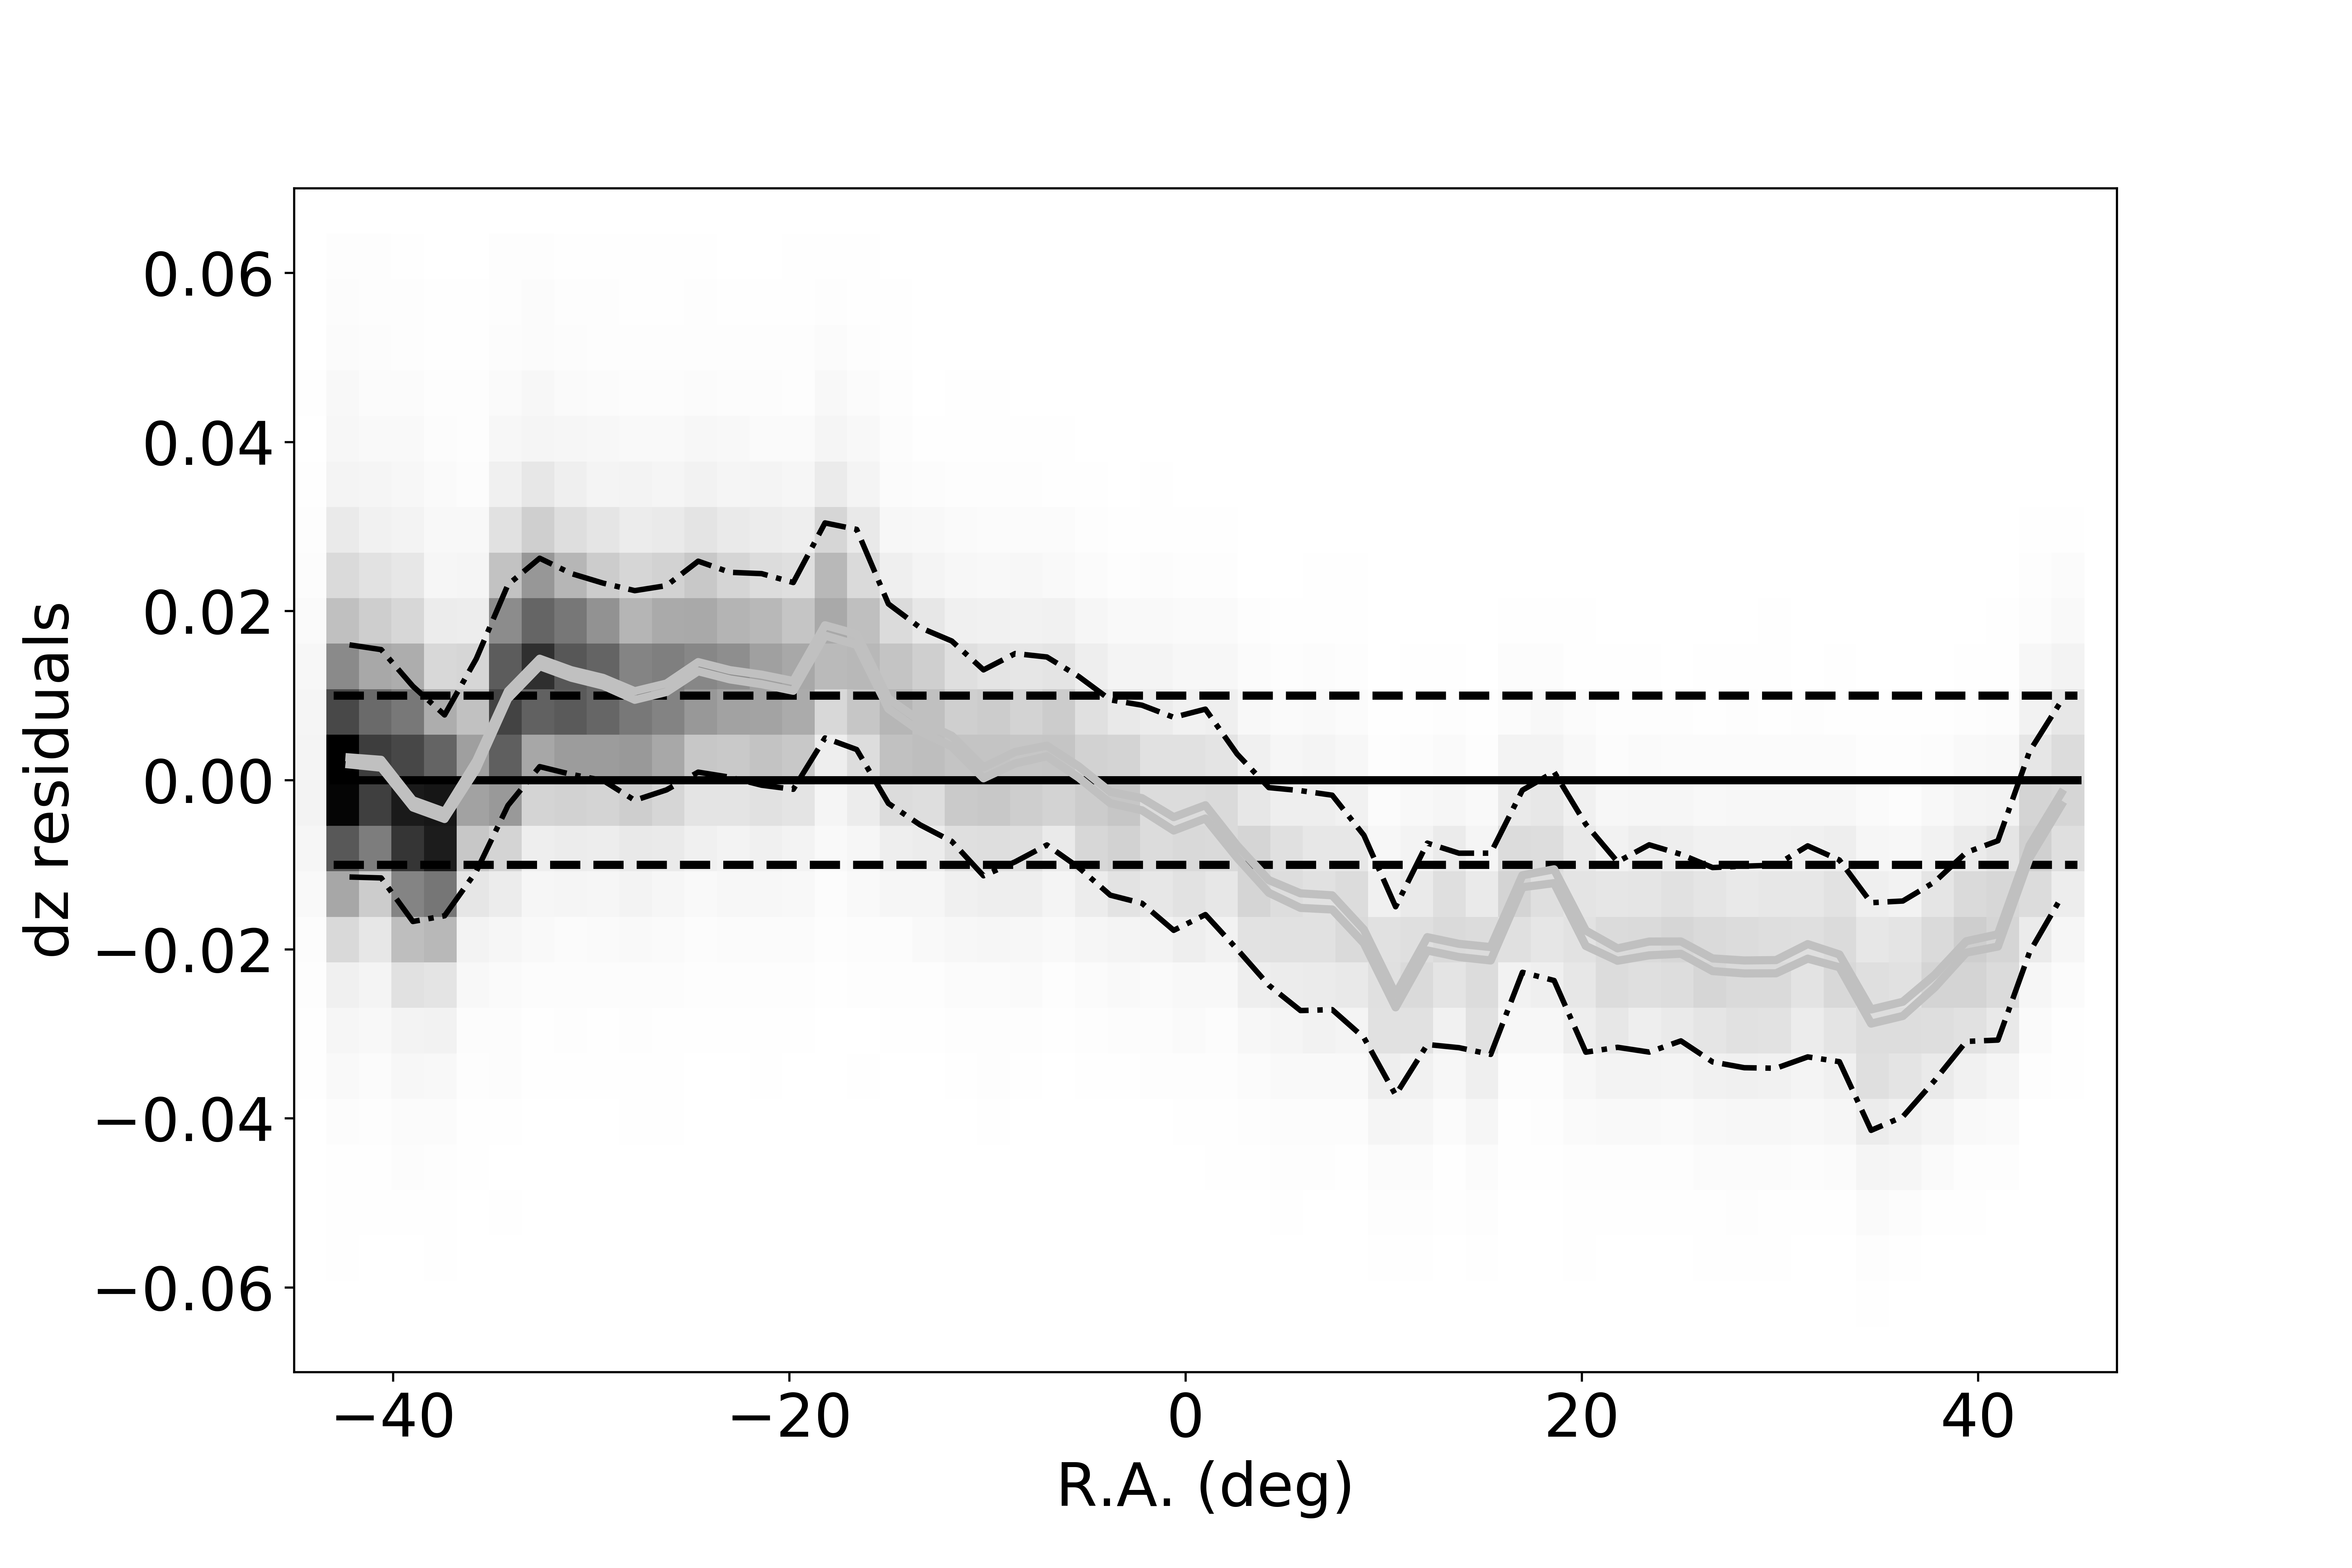
\includegraphics[width=7cm]{figures/colorResidDES2bright_dz_RA_Hess.png}
    \centering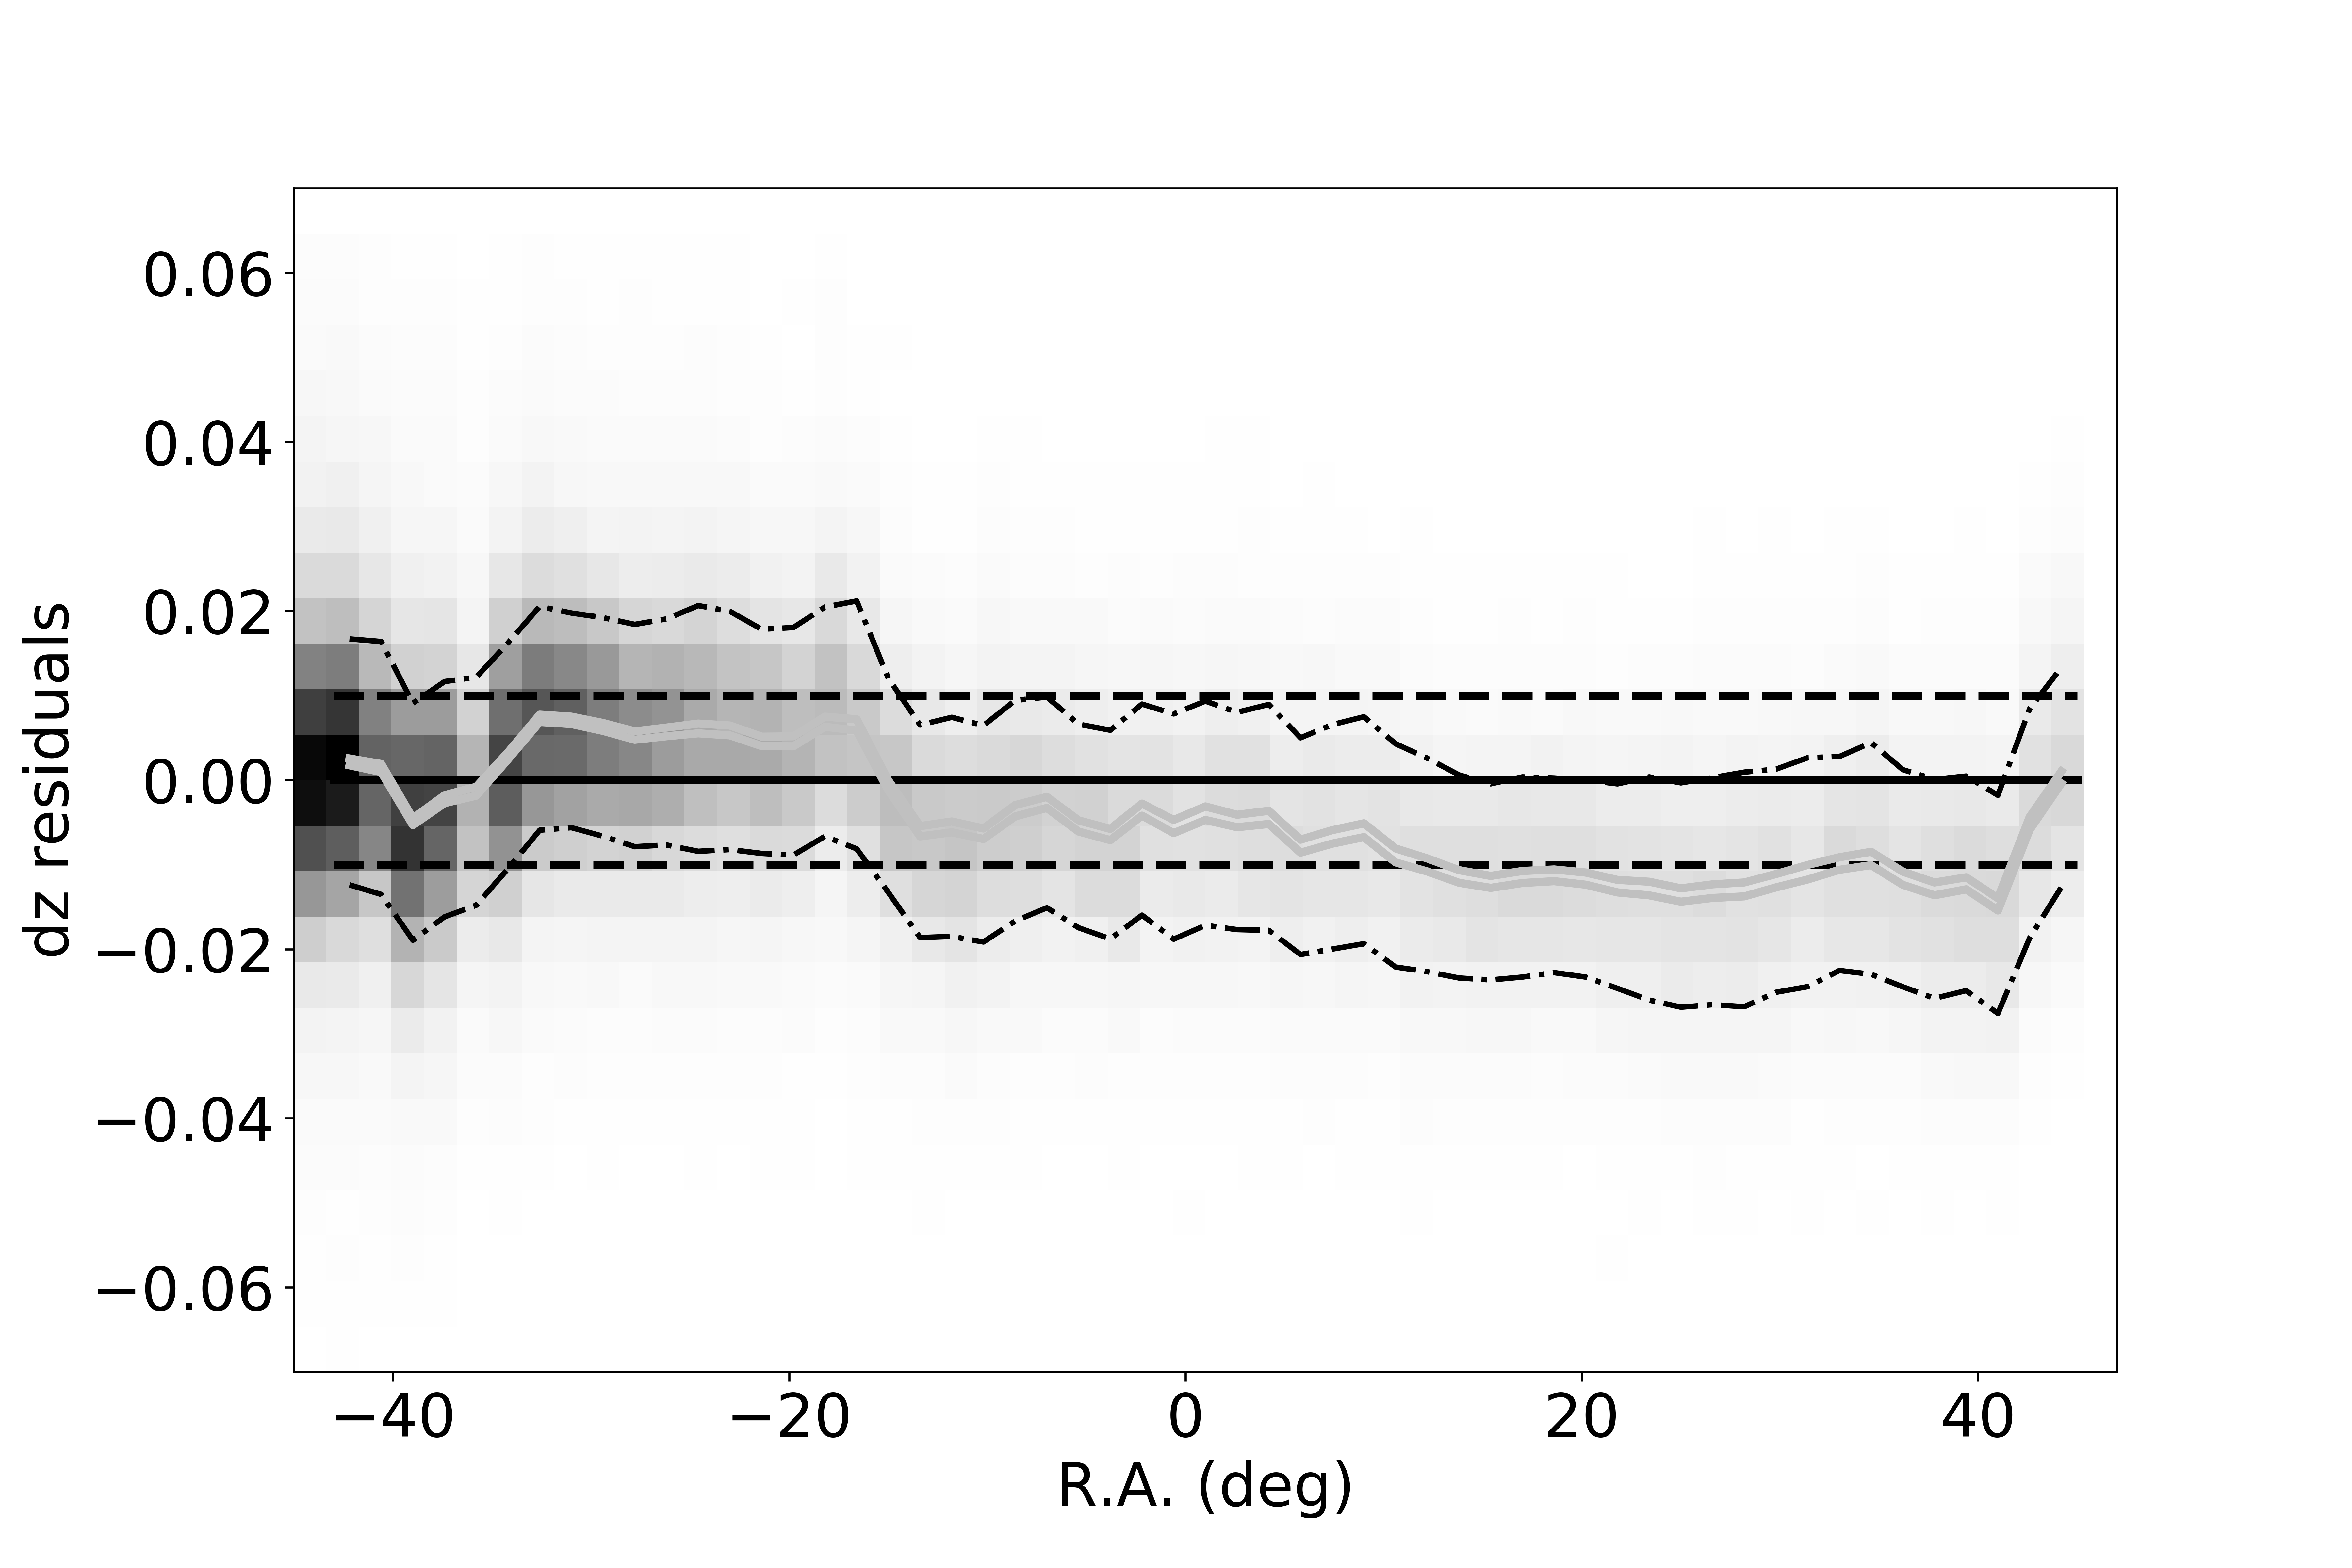
\includegraphics[width=7cm]{figures/colorResidPSbright_dz_RA_Hess.png}
\caption{A comparison of the magnitude differences between the SDSS v3.4 catalog
and DES (left) and Pan-STARRS (right) catalogs, for the $riz$ bands.}
\label{fig:DESPSRA}
\end{figure}

\begin{figure}
    \centering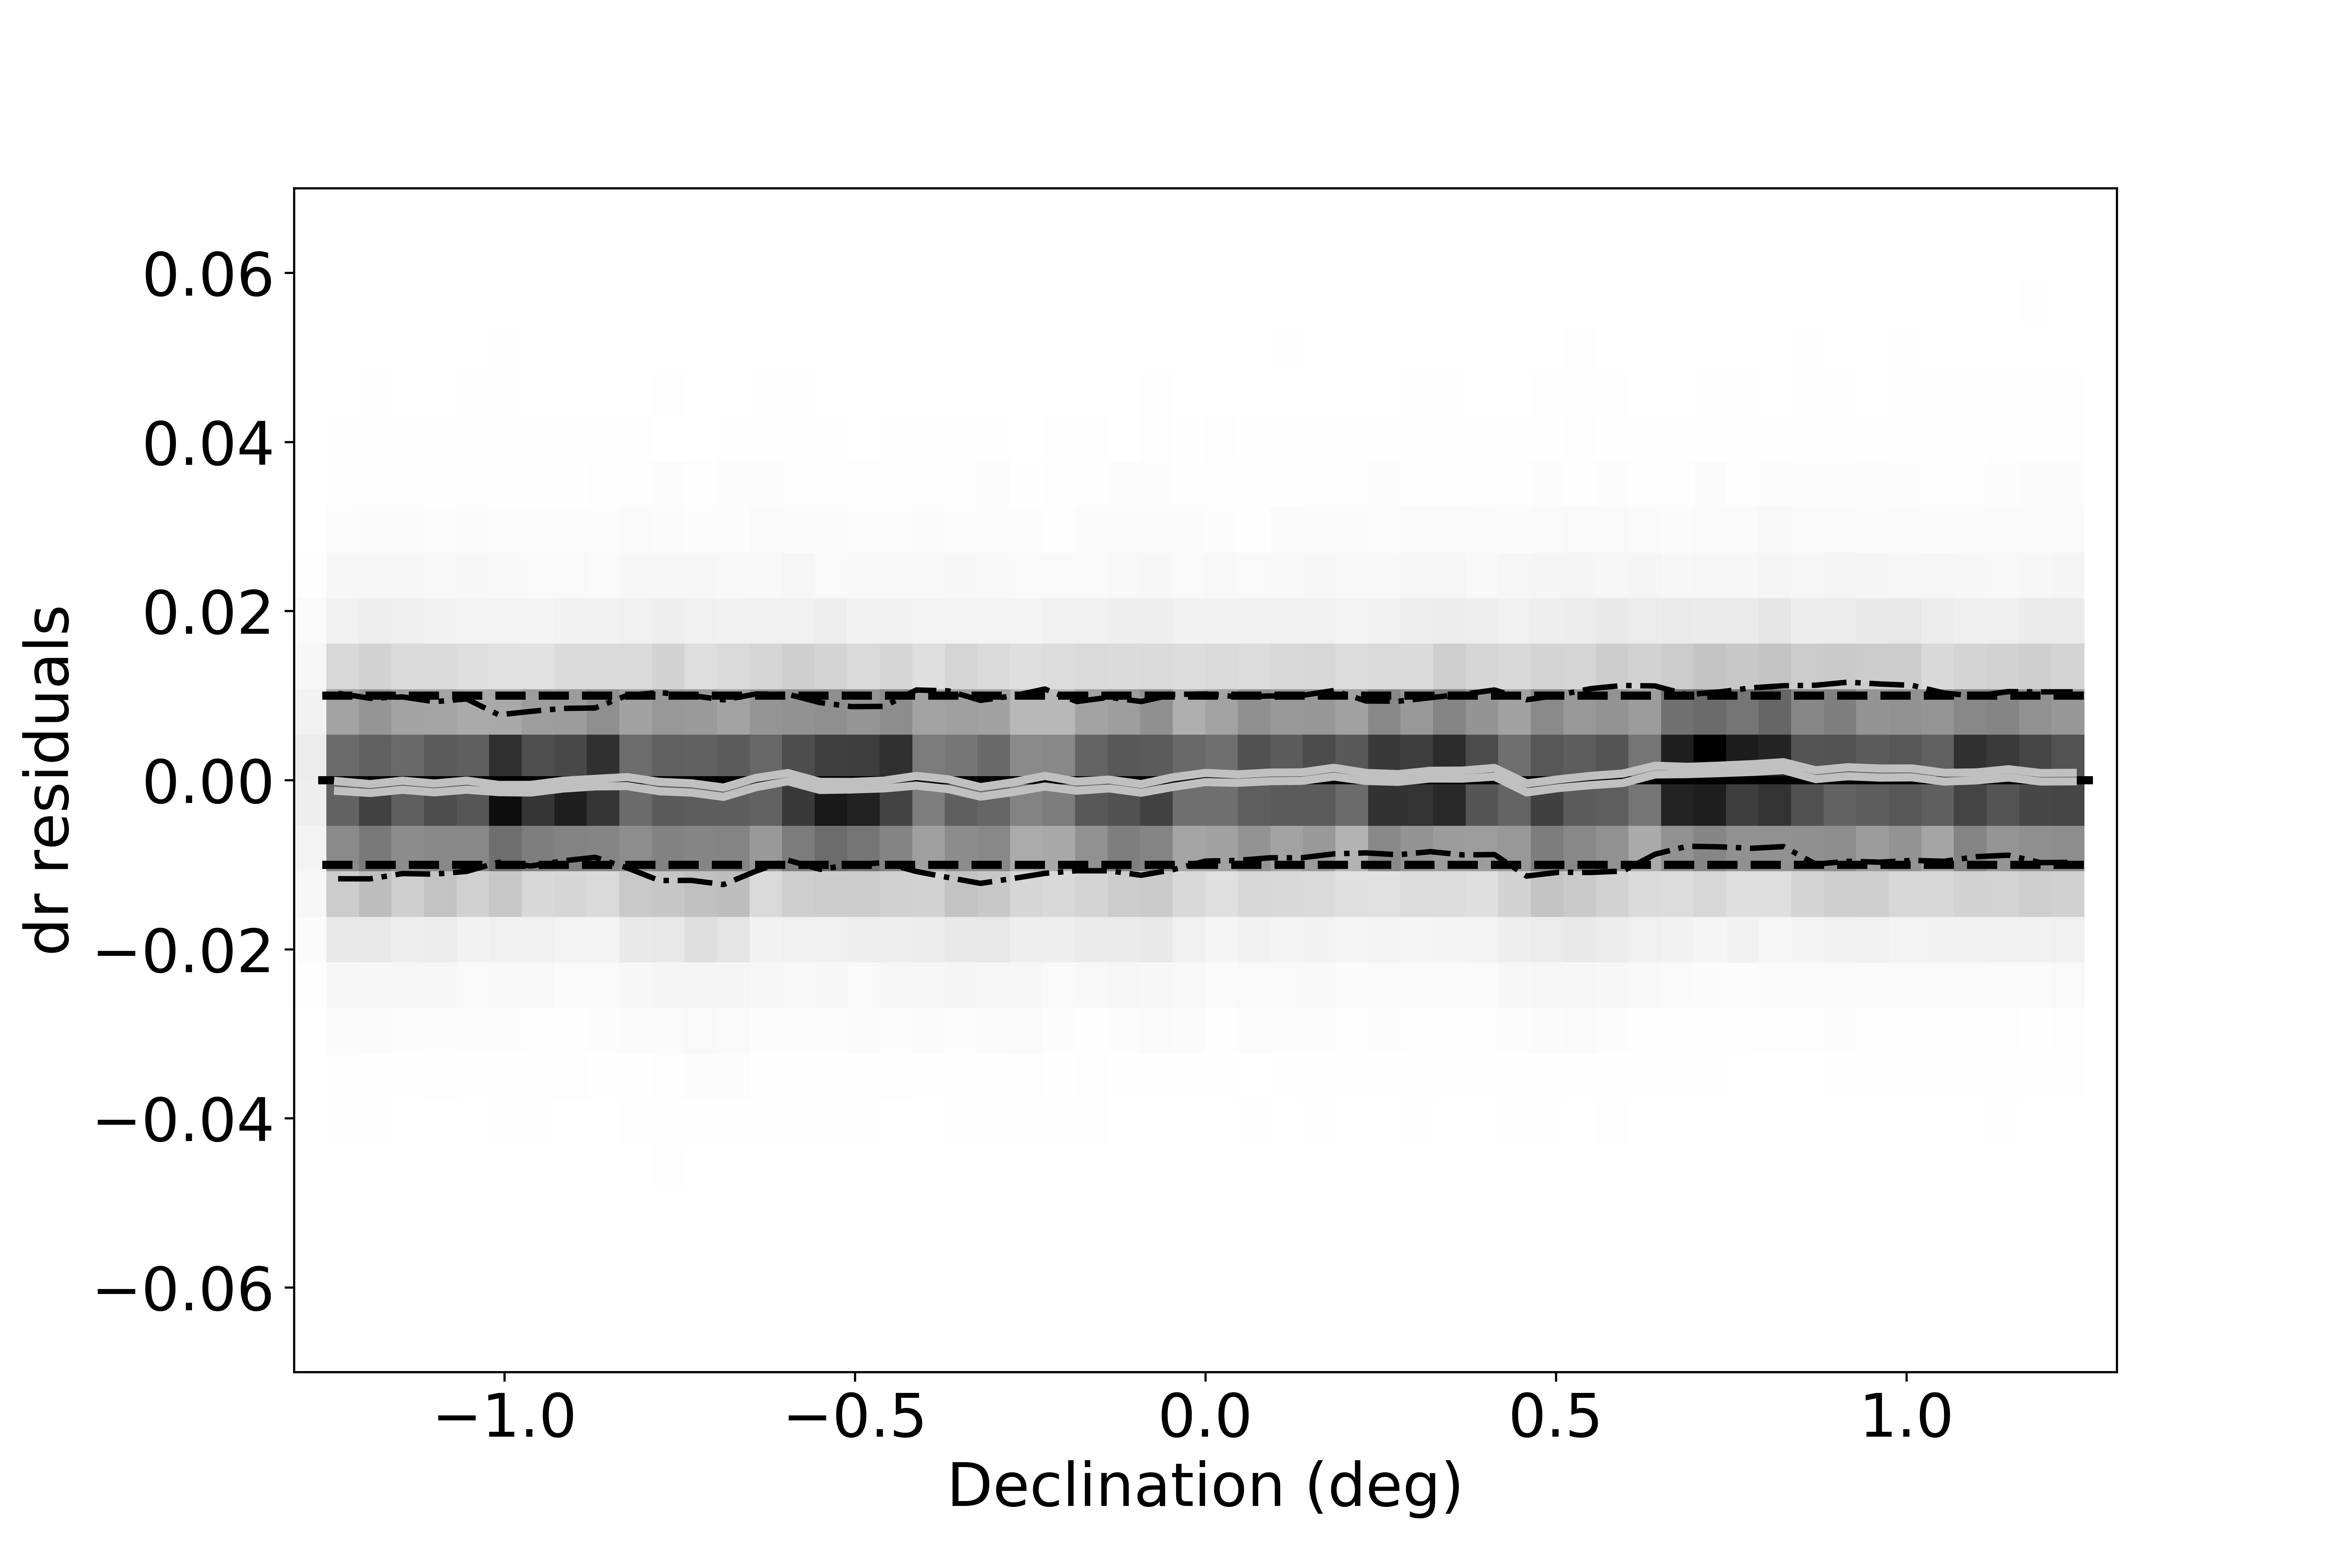
\includegraphics[width=7cm]{figures/colorResidDES2bright_dr_Dec_Hess.png}
    \centering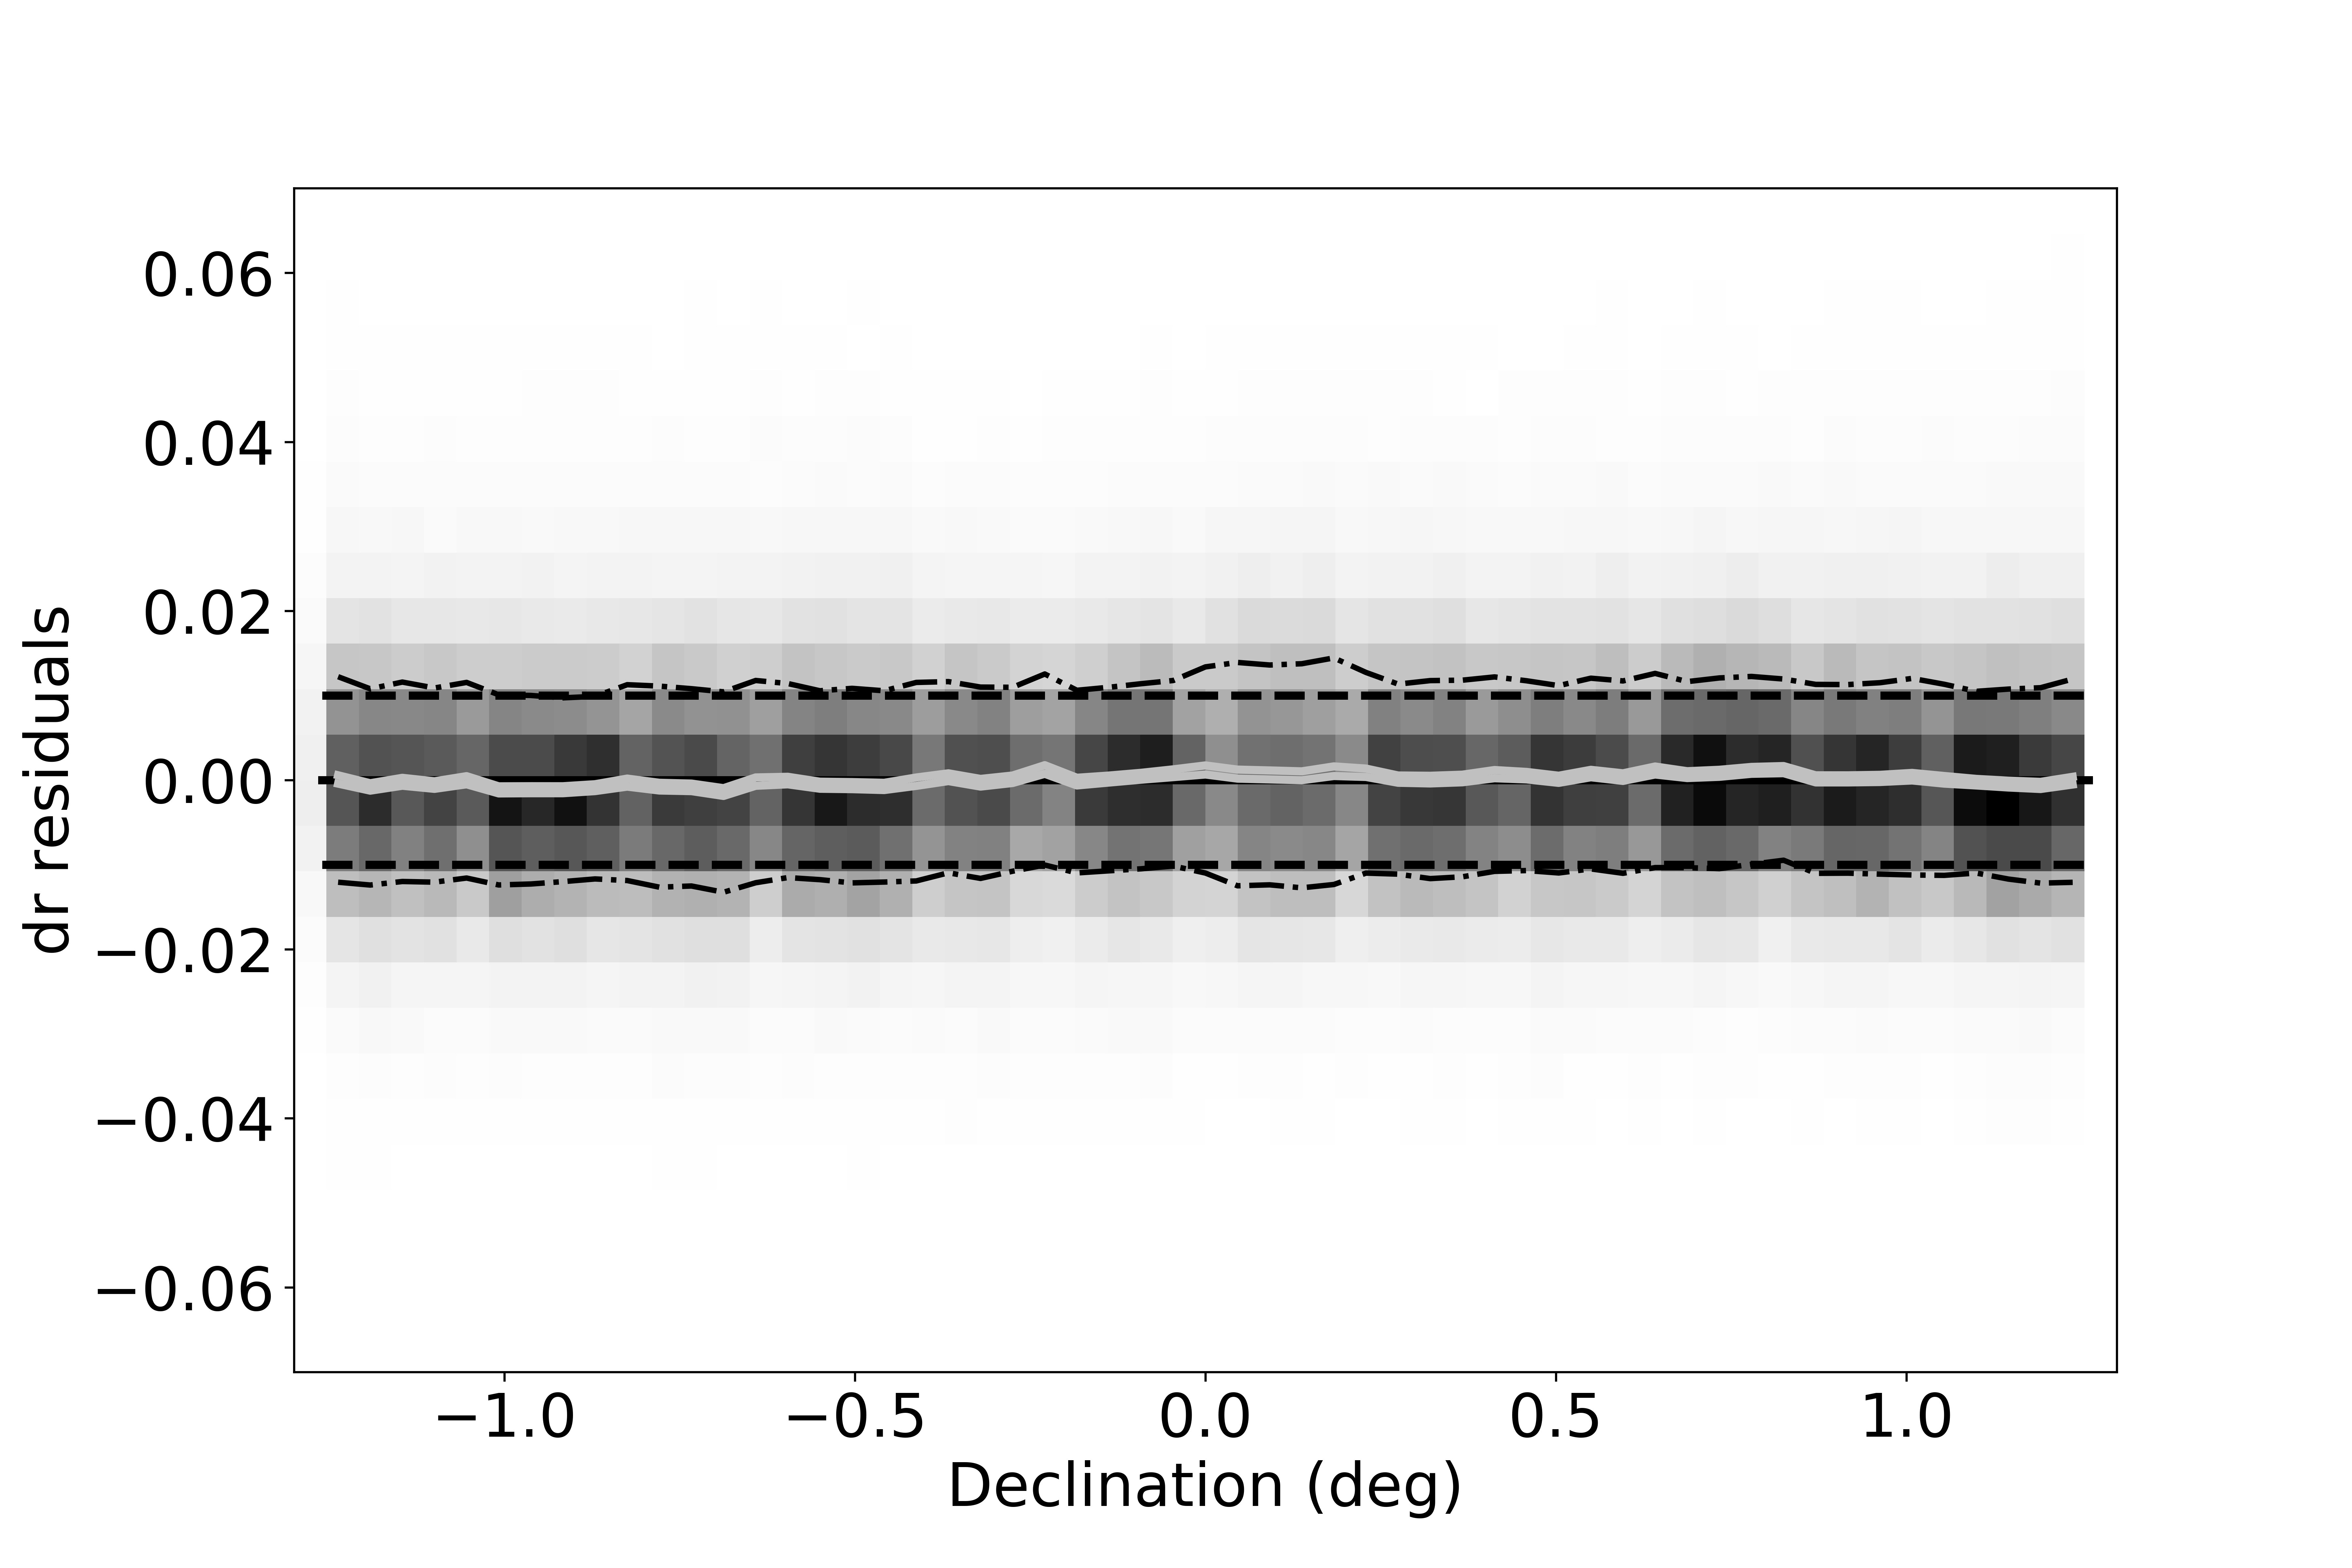
\includegraphics[width=7cm]{figures/colorResidPSbright_dr_Dec_Hess.png}
    \centering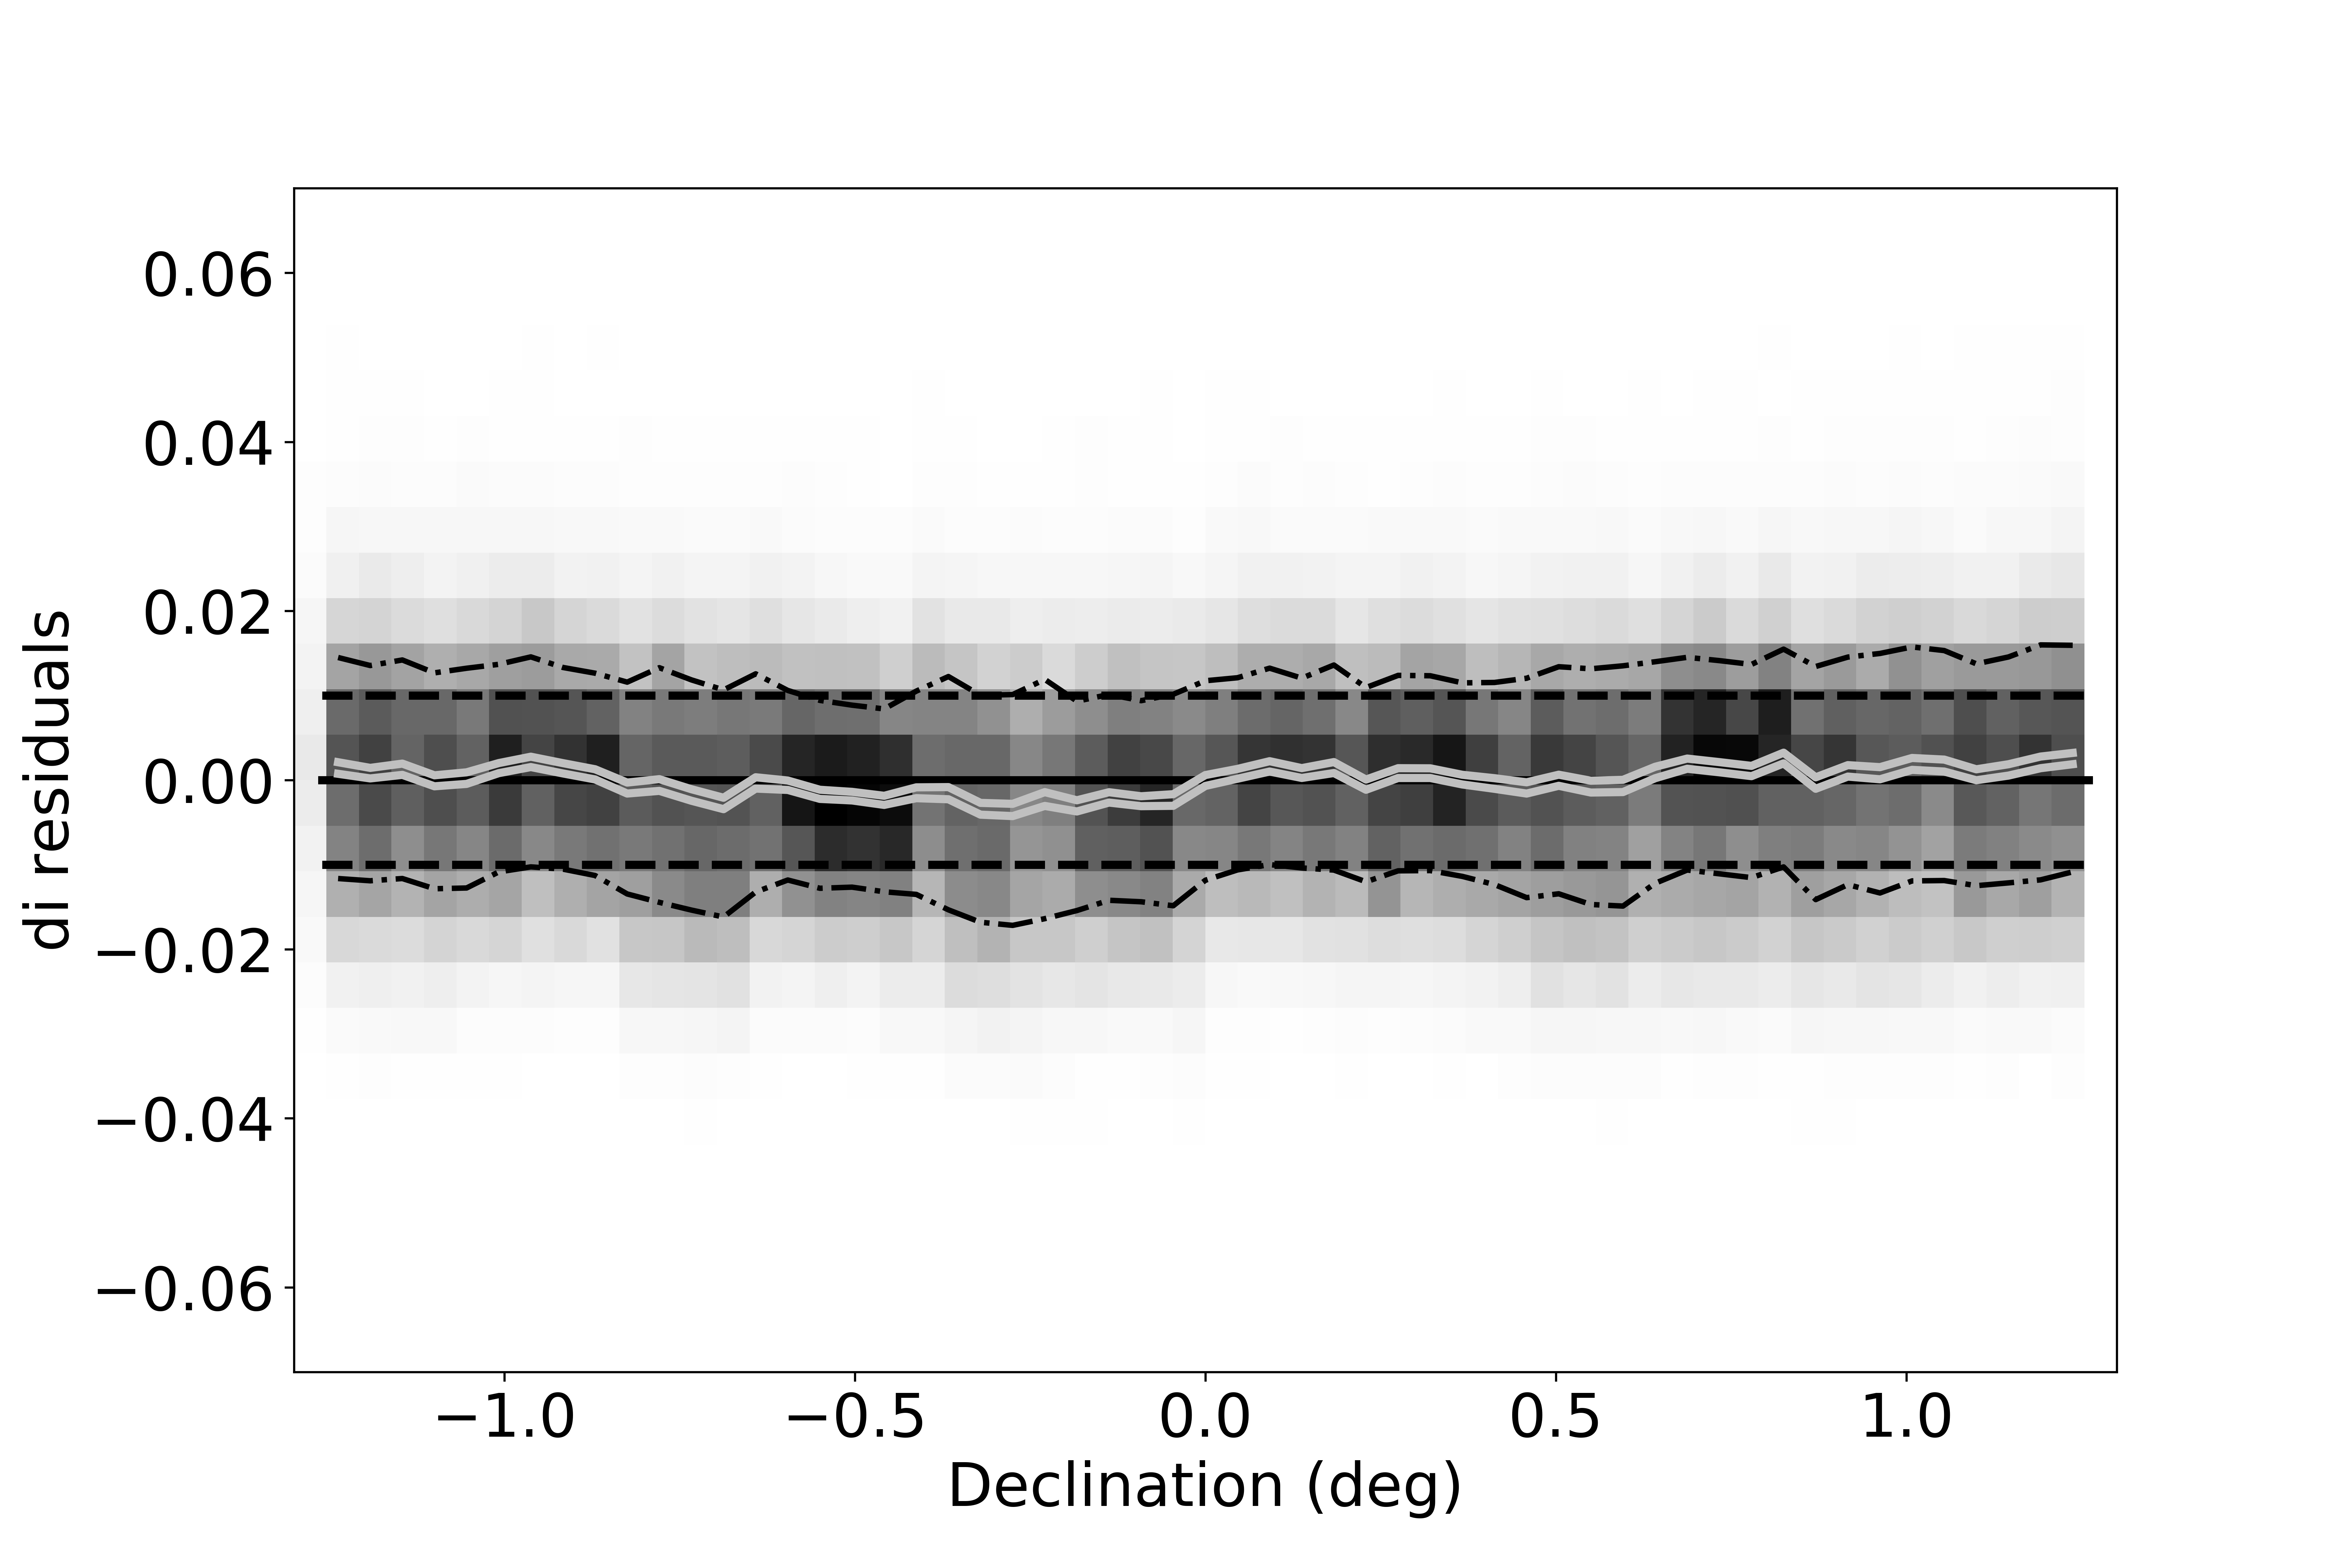
\includegraphics[width=7cm]{figures/colorResidDES2bright_di_Dec_Hess.png}
    \centering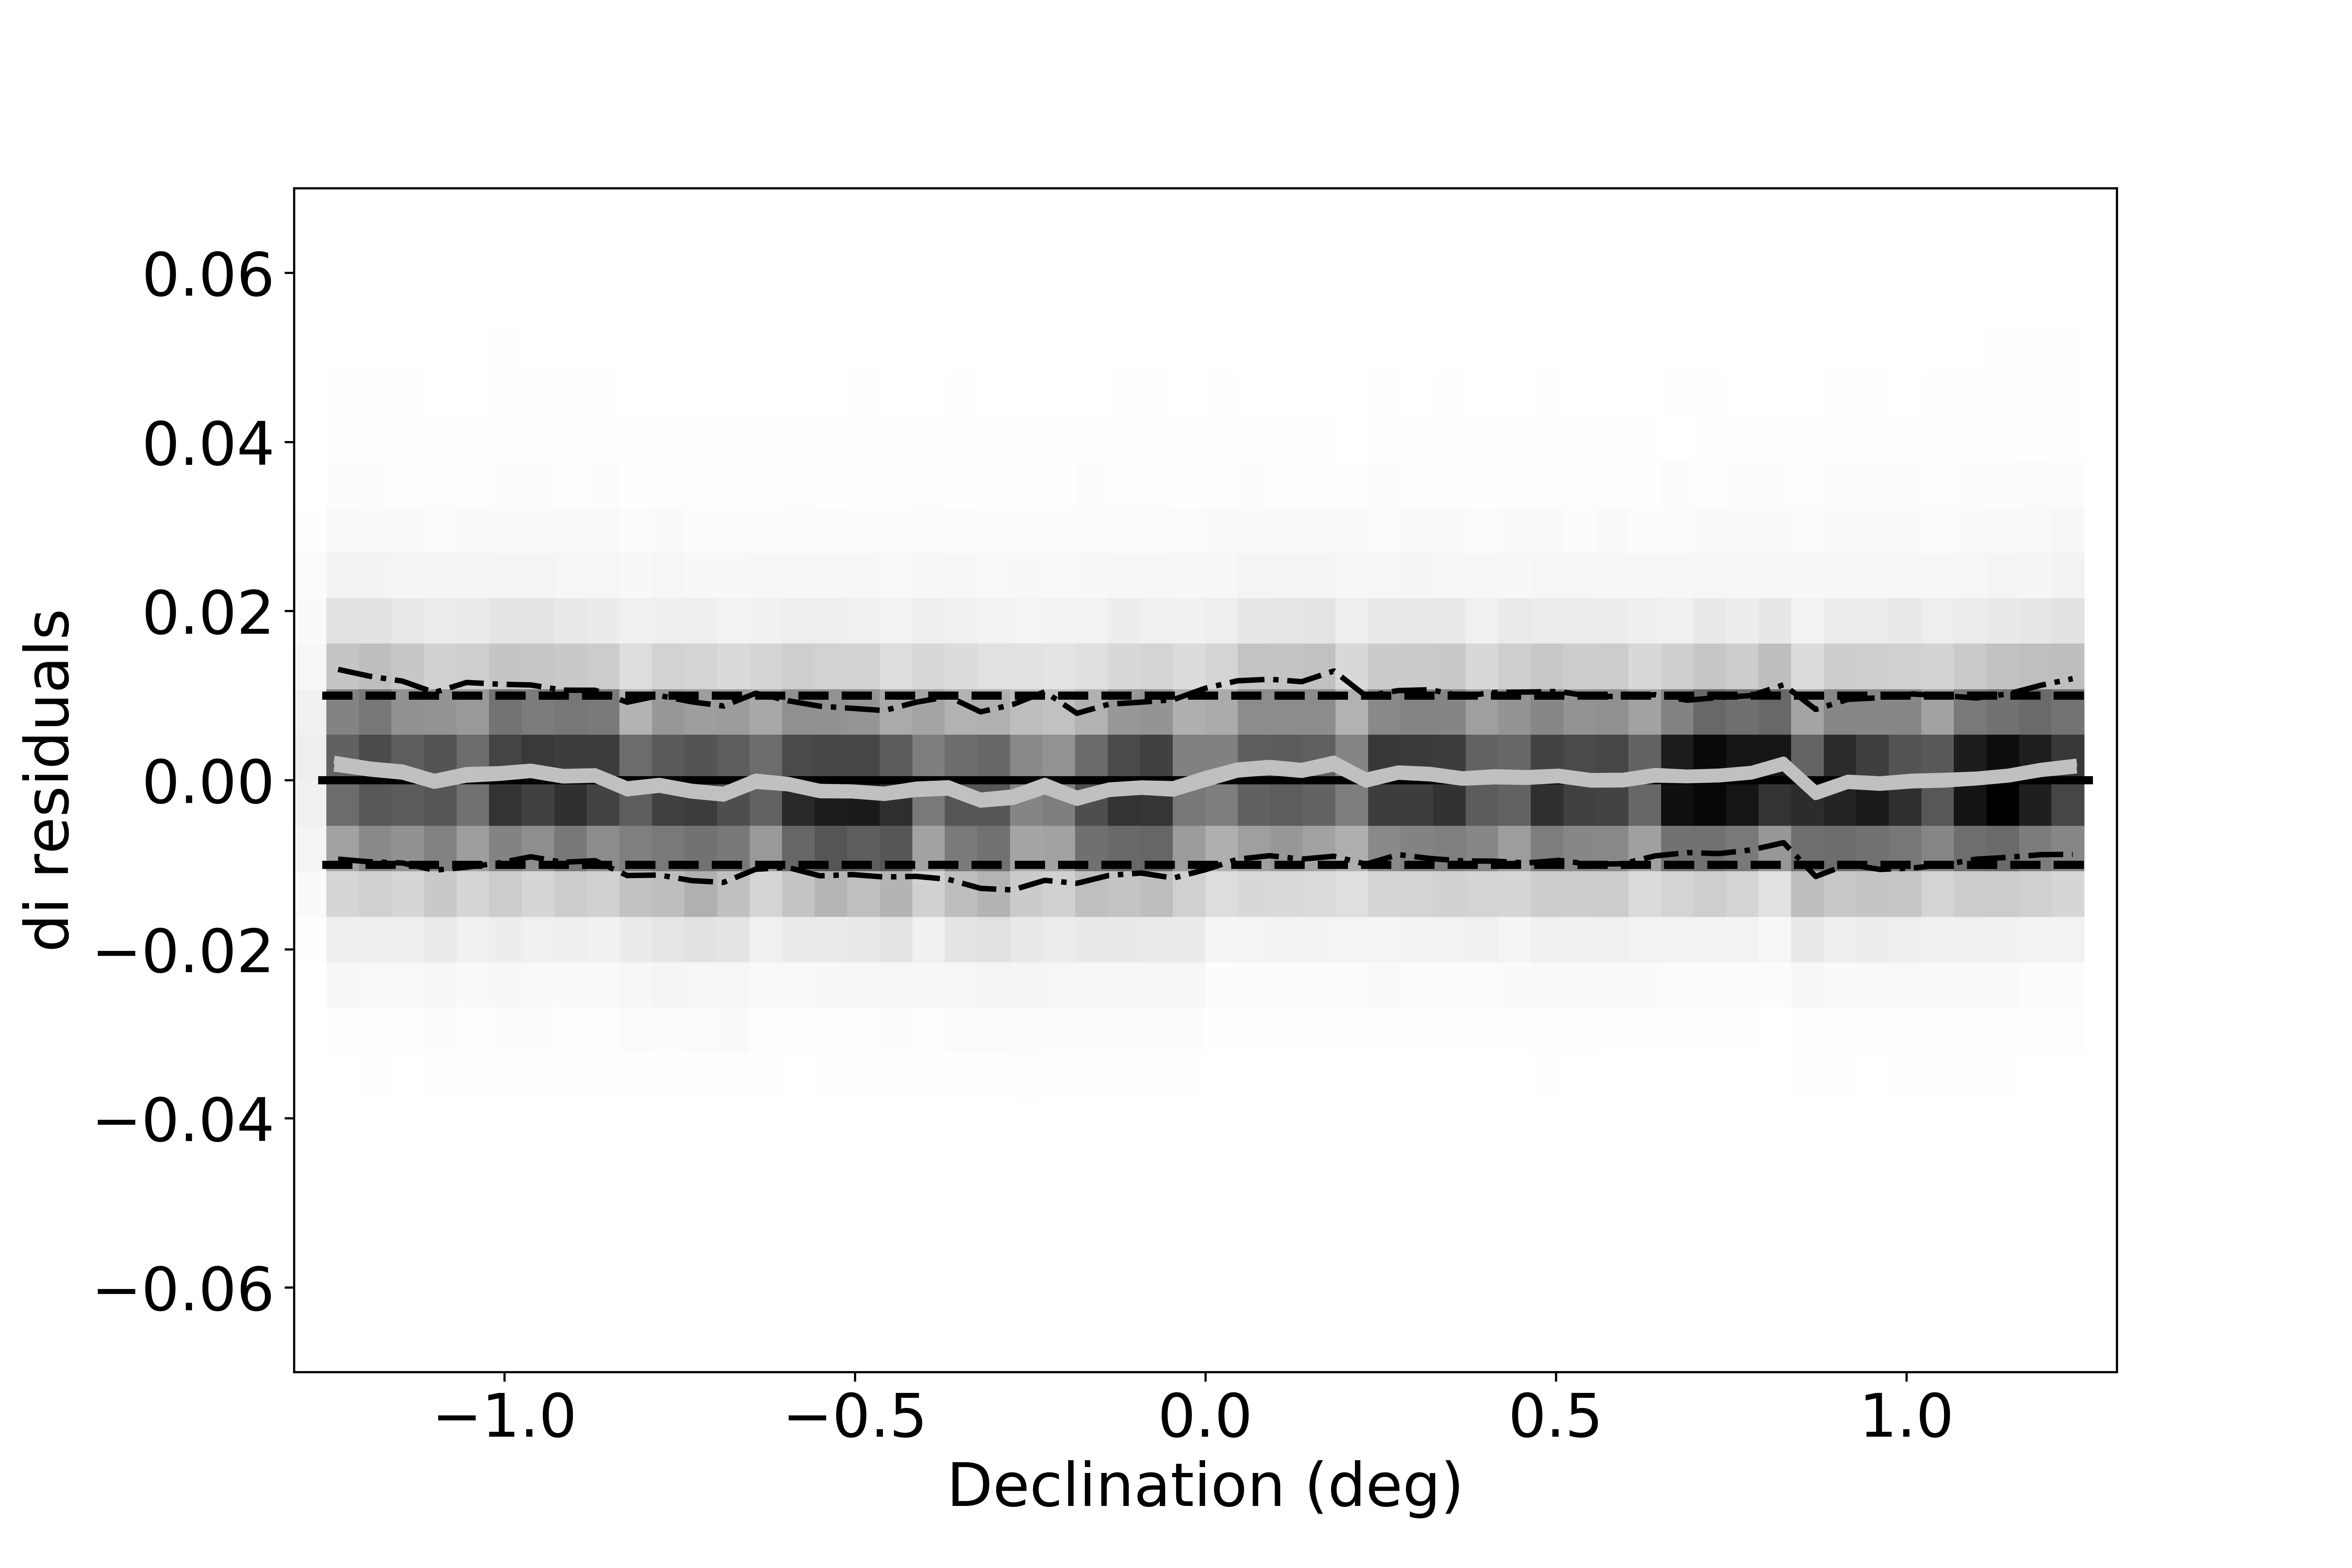
\includegraphics[width=7cm]{figures/colorResidPSbright_di_Dec_Hess.png}
    \centering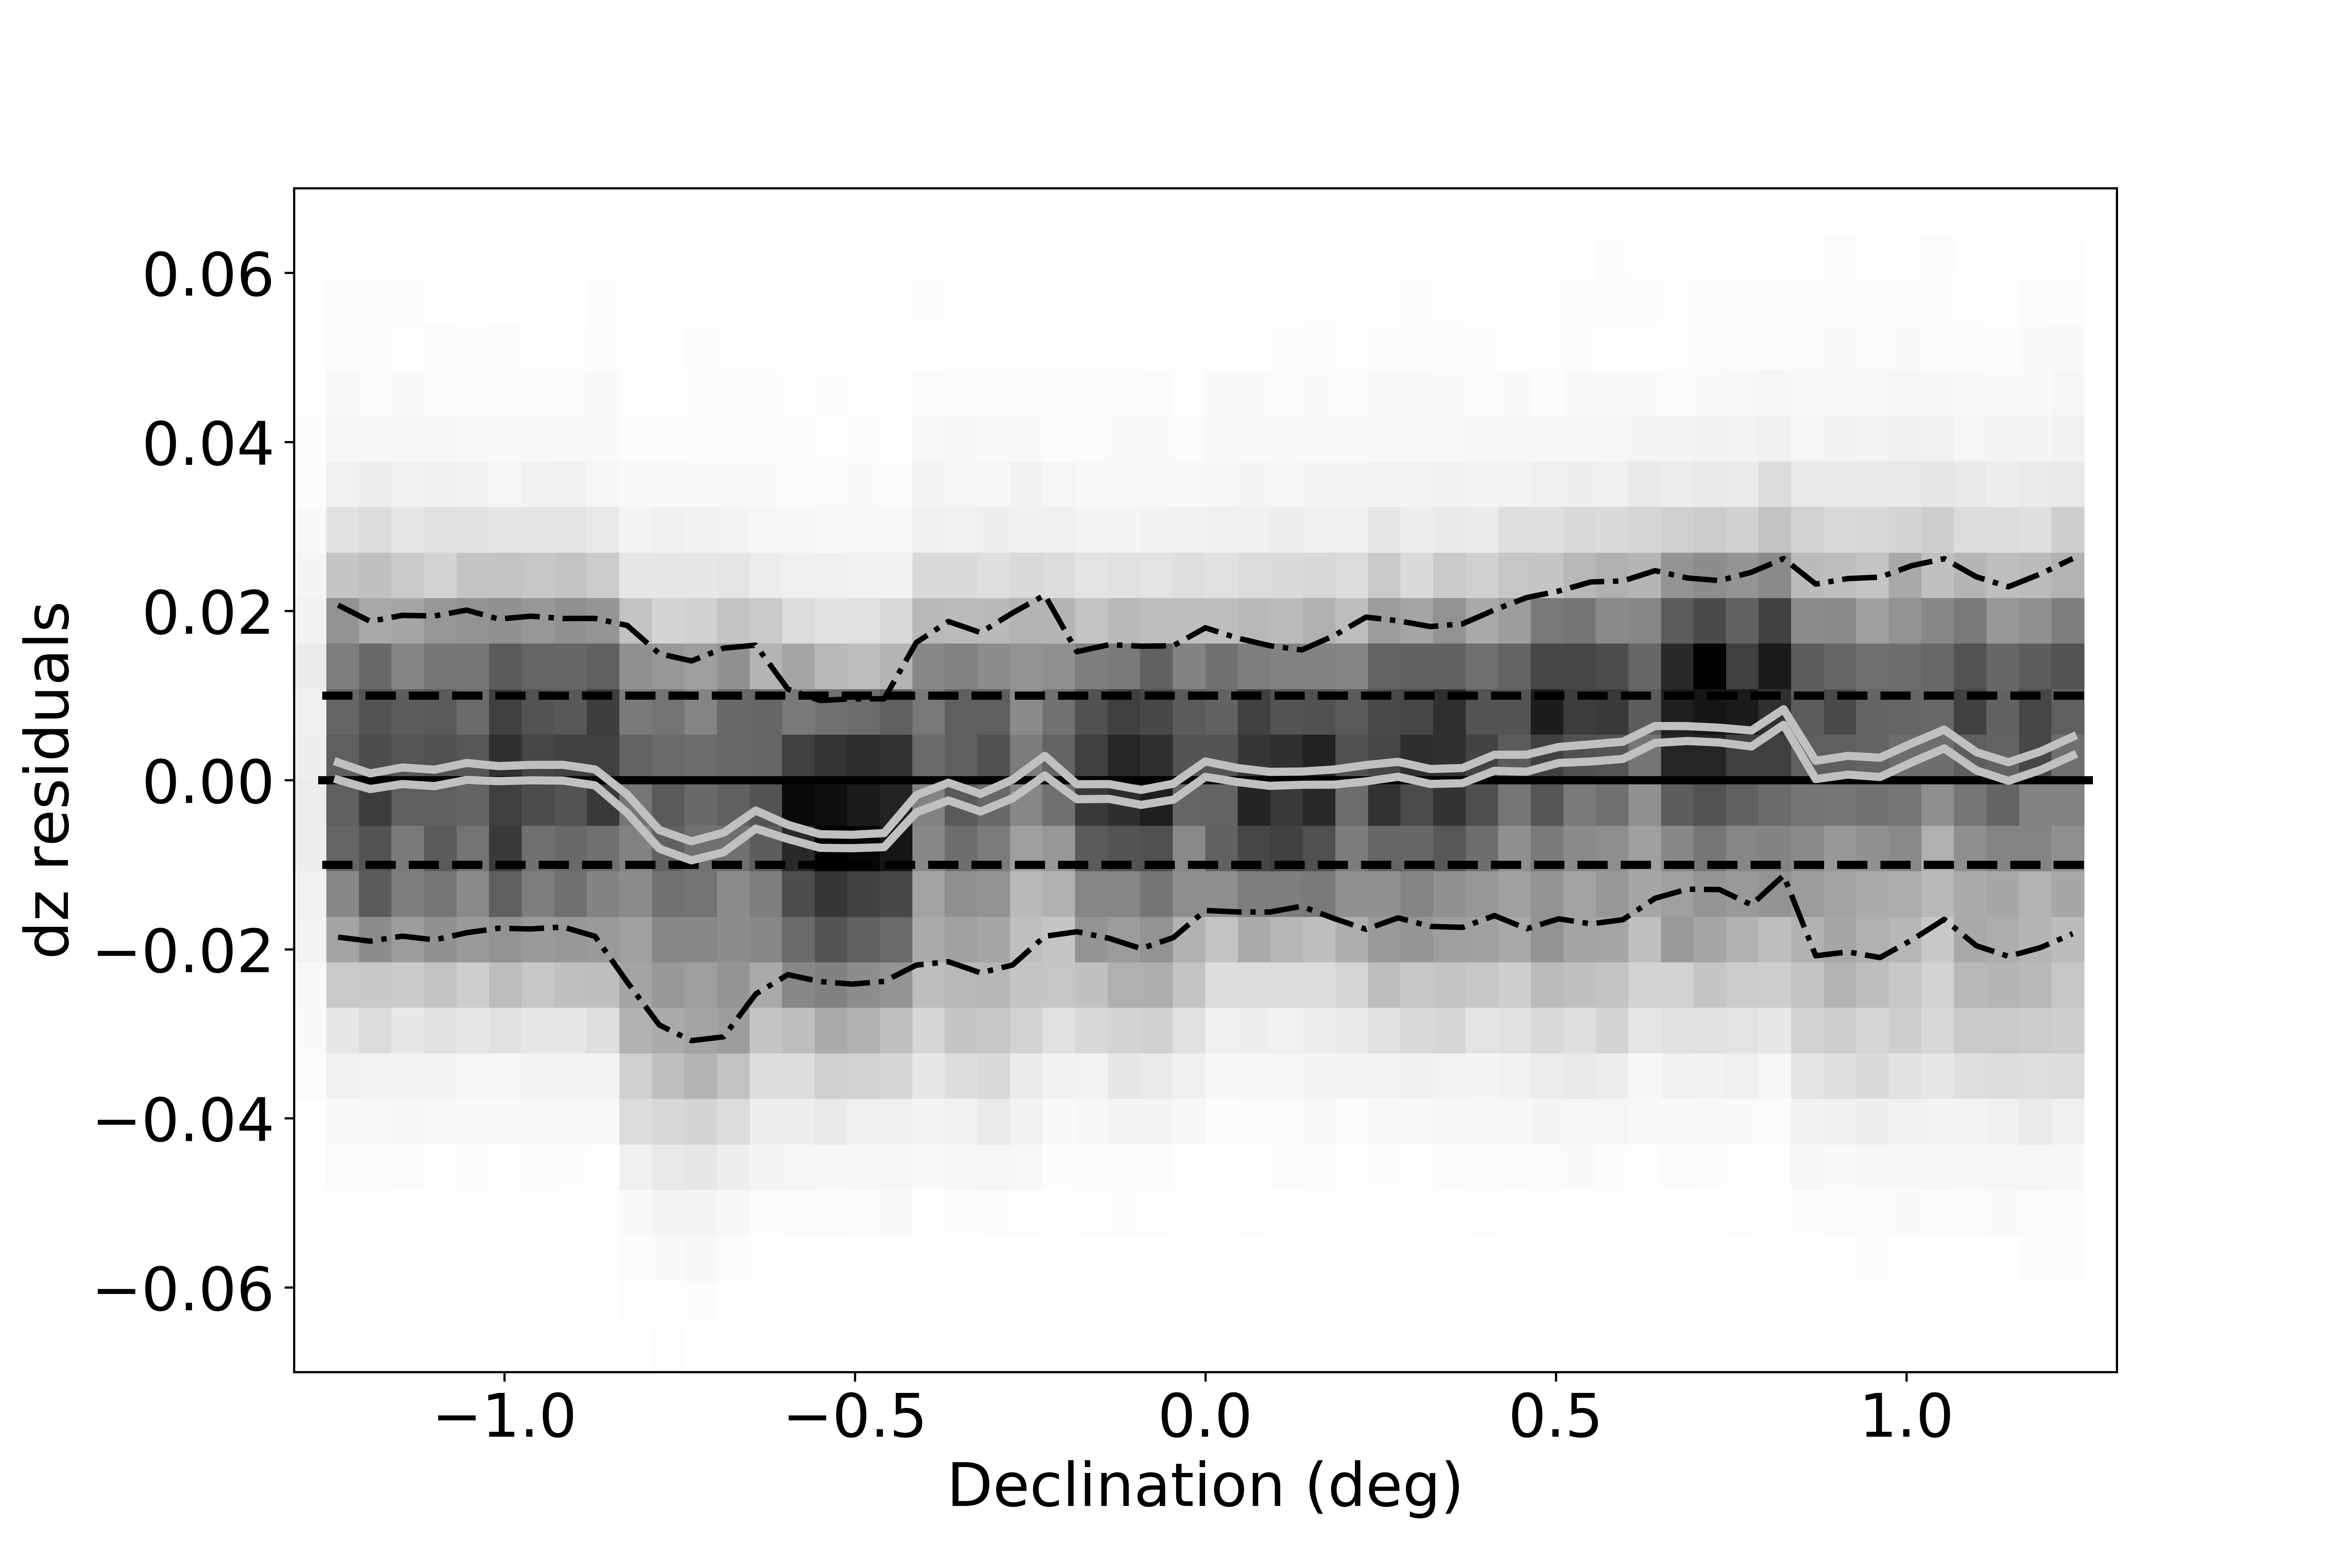
\includegraphics[width=7cm]{figures/colorResidDES2bright_dz_Dec_Hess.png}
    \centering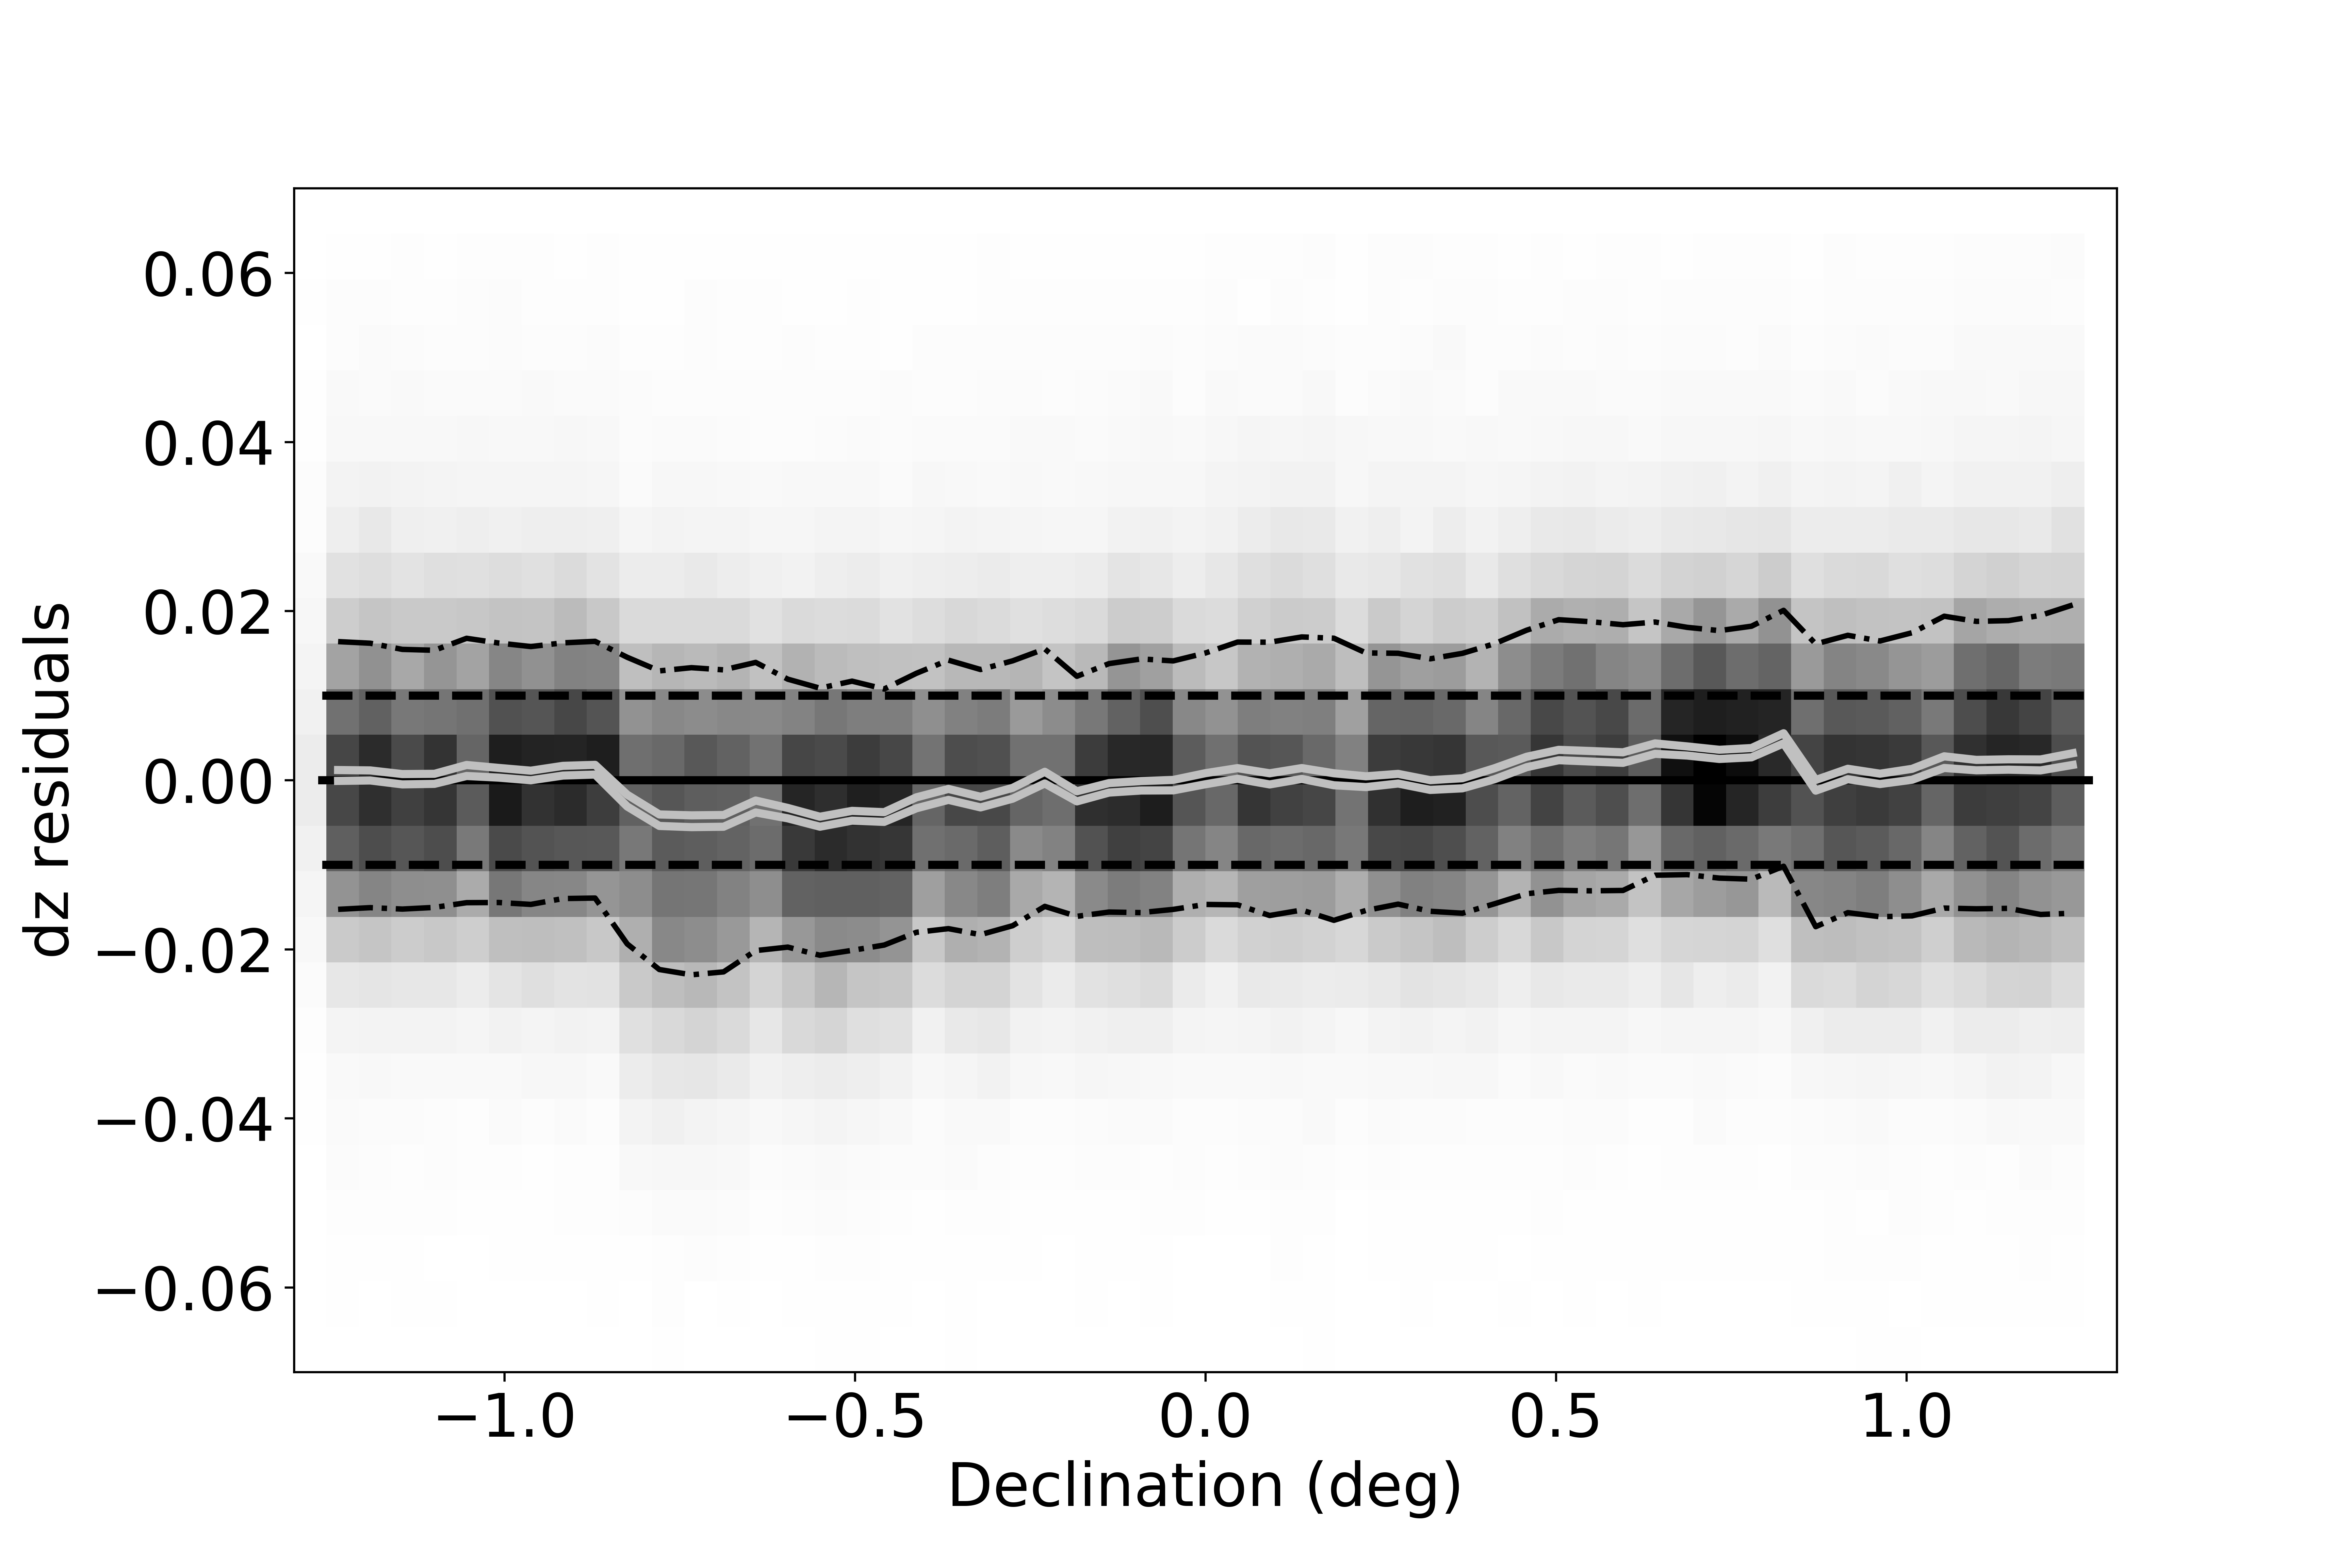
\includegraphics[width=7cm]{figures/colorResidPSbright_dz_Dec_Hess.png}
\caption{Analogous to Figure~\ref{fig:DESPSRA}, except that magnitude differences
are binned by Declination.}
\label{fig:DESPSDec}
\end{figure}

\begin{figure}
    \centering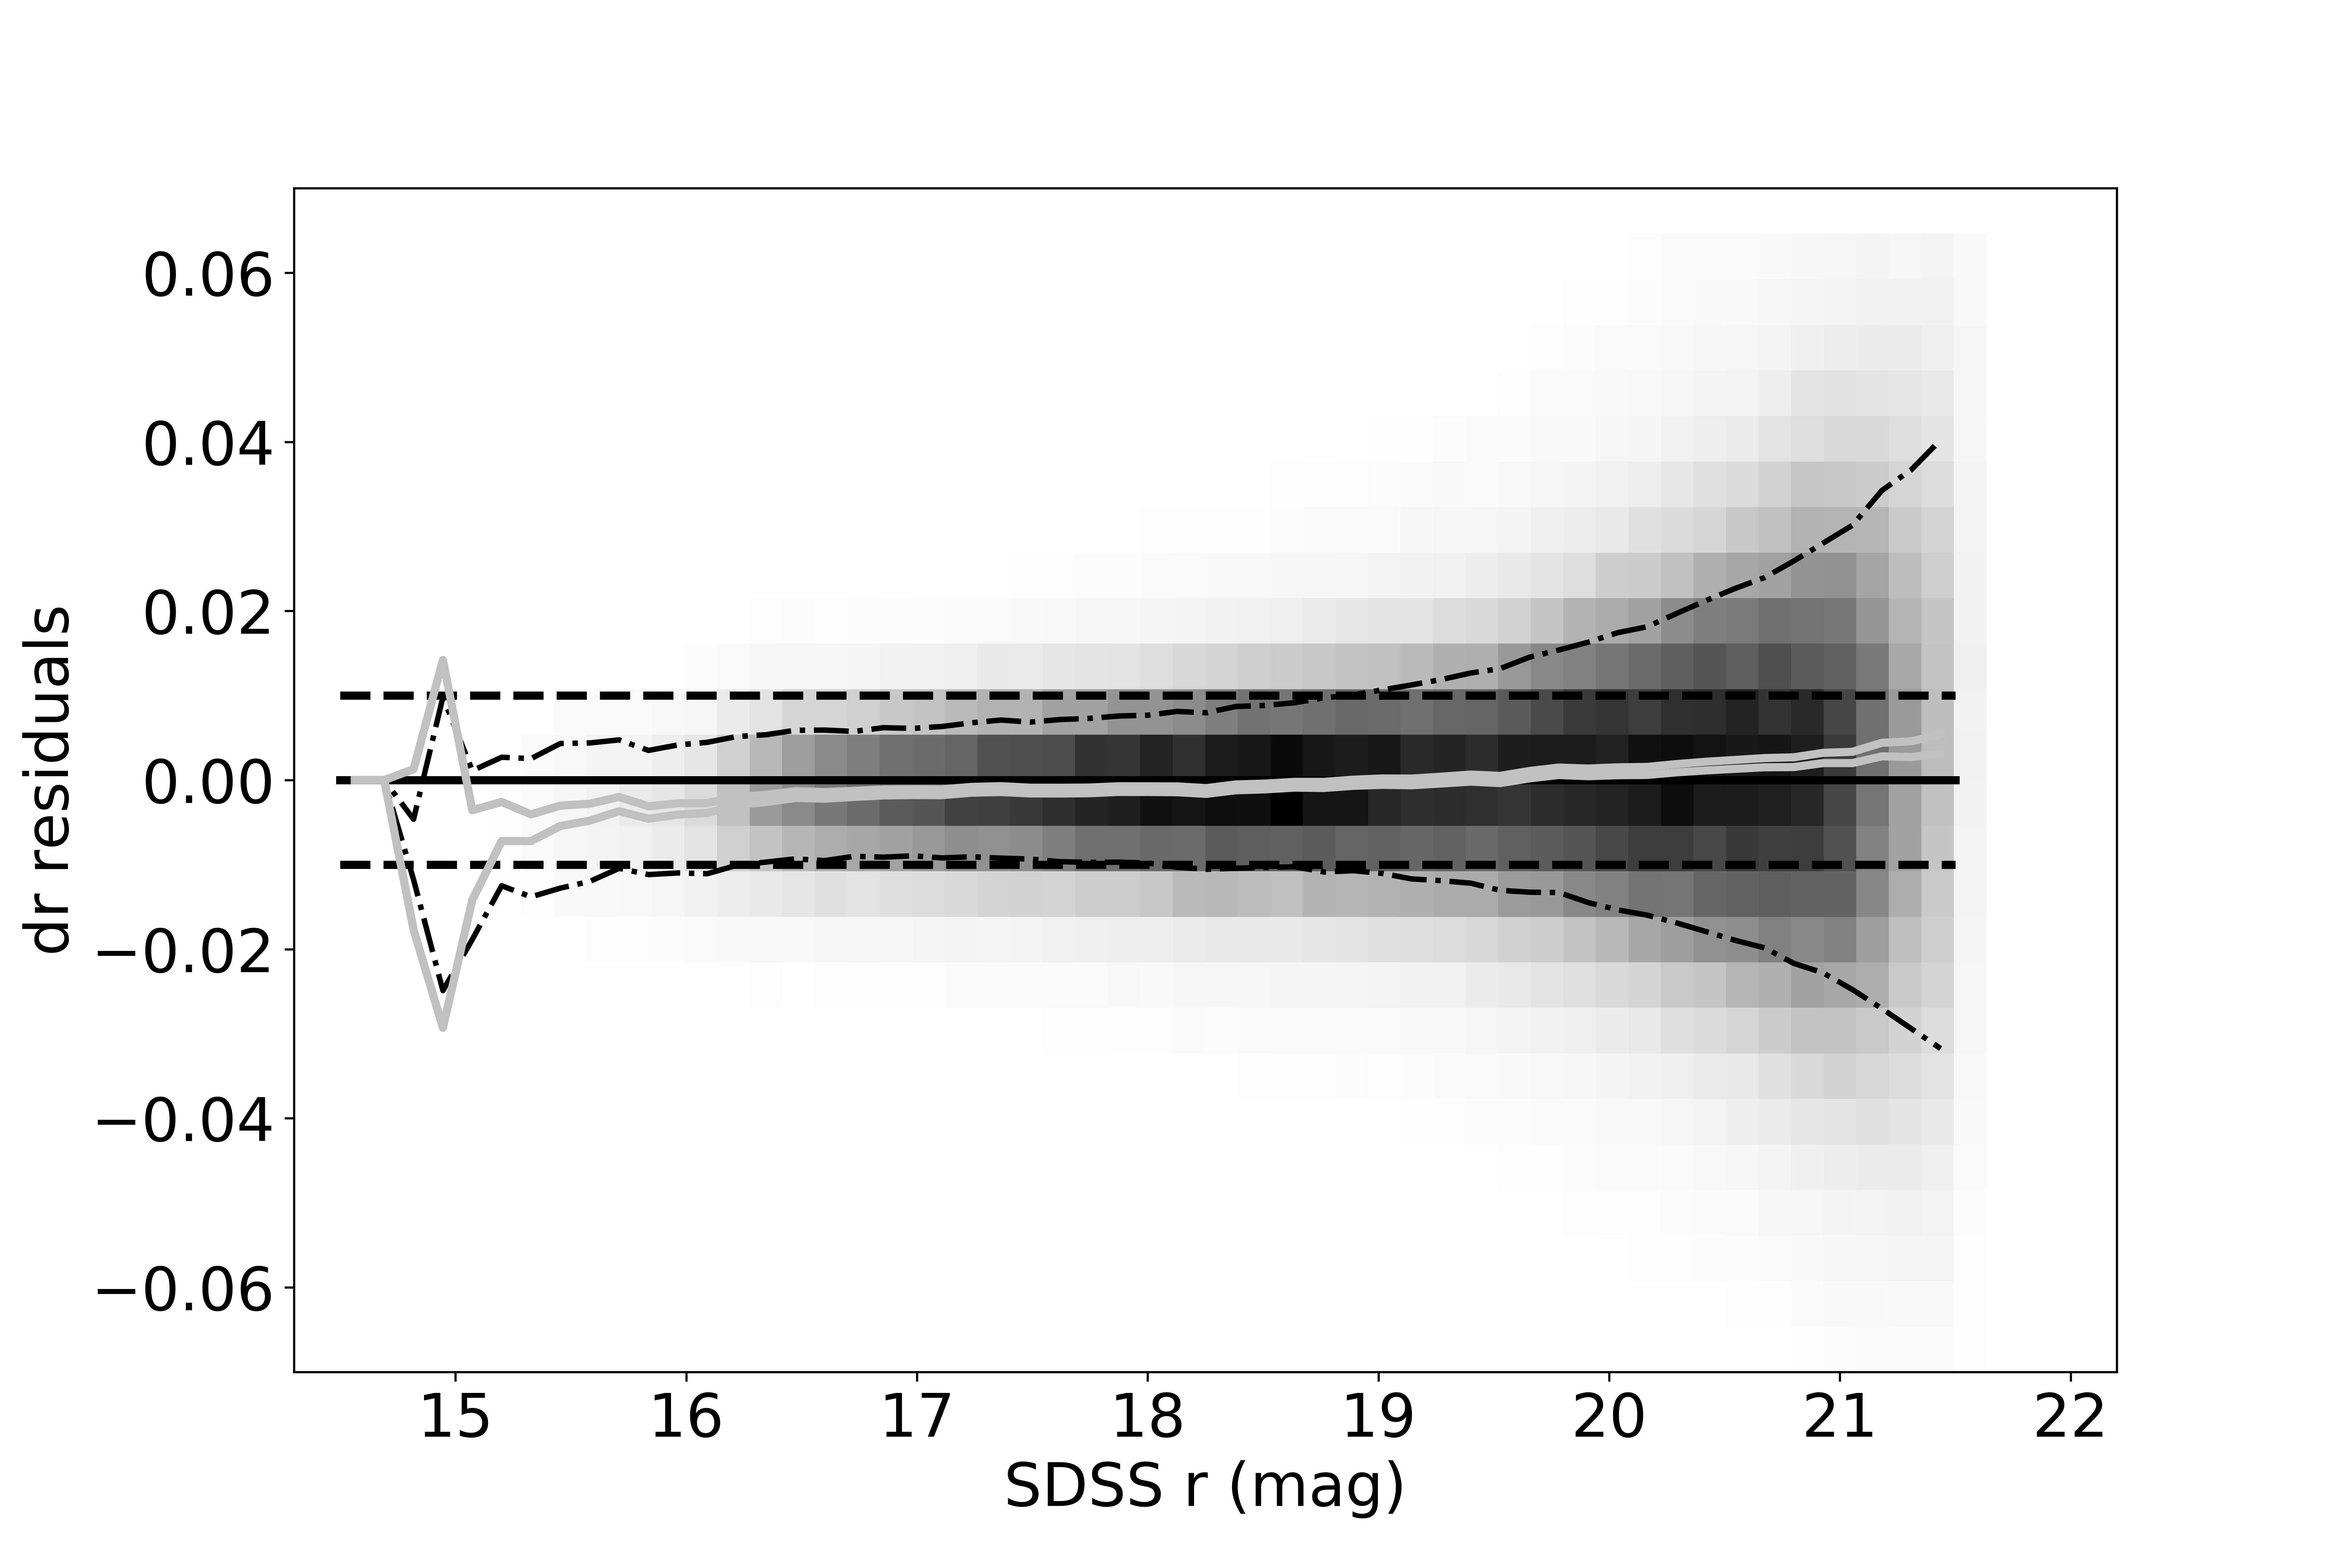
\includegraphics[width=7cm]{figures/colorResidDES2_dr_rmag_Hess.png}
    \centering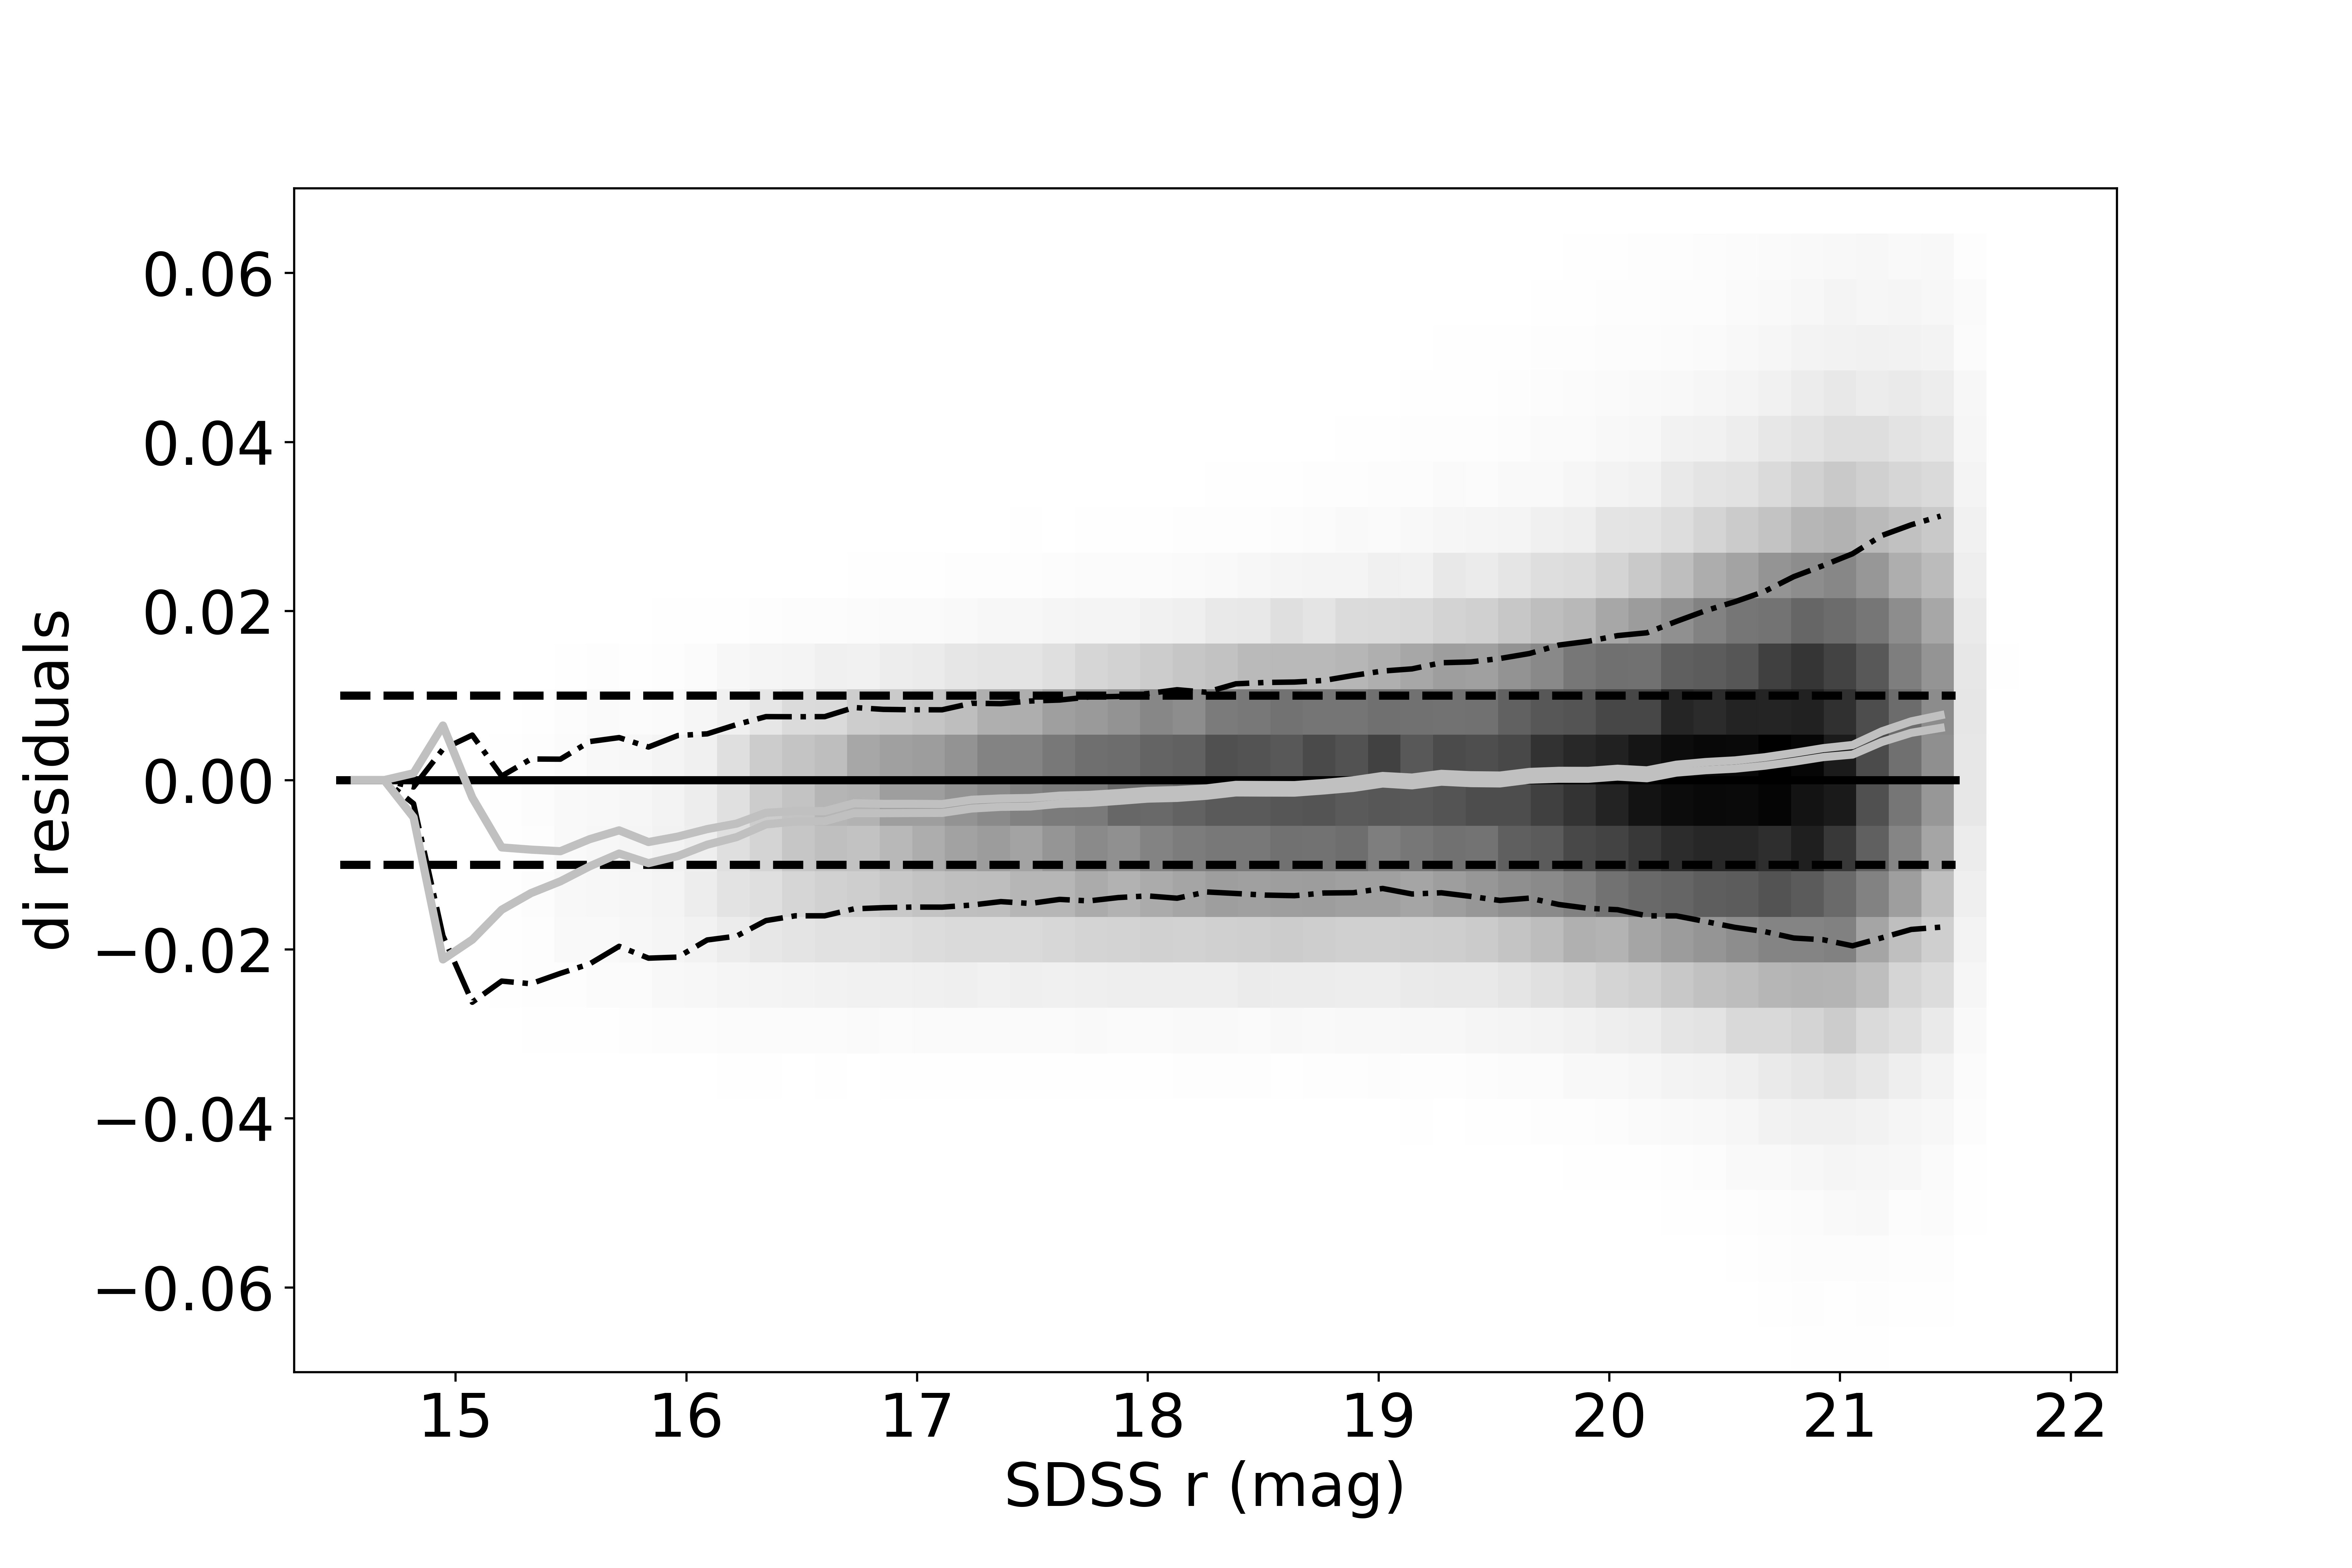
\includegraphics[width=7cm]{figures/colorResidDES2_di_rmag_Hess.png} 
\caption{A comparison of the magnitude differences between the SDSS v3.4 catalog
and DES catalog, for the $r$ and $i$ bands. Note the good agreement even at the
faint end ($20<r<21$), where Gaia Gmag magnitudes appear too faint by about
0.02 mag (see Figure~\ref{fig:gaiaJump}).} 
\label{fig:drVSr}
\end{figure}



\subsection{Comparison of the new v3.4 SDSS catalog and $u$ band data from the CFIS catalog  \label{sec:CFIStest}} 


CFIS: as a function of RA, the maximum u band zeropoint offset is limited to $<0.02$ mag,
           with rms of 17 millimag. 


\begin{figure}
    \centering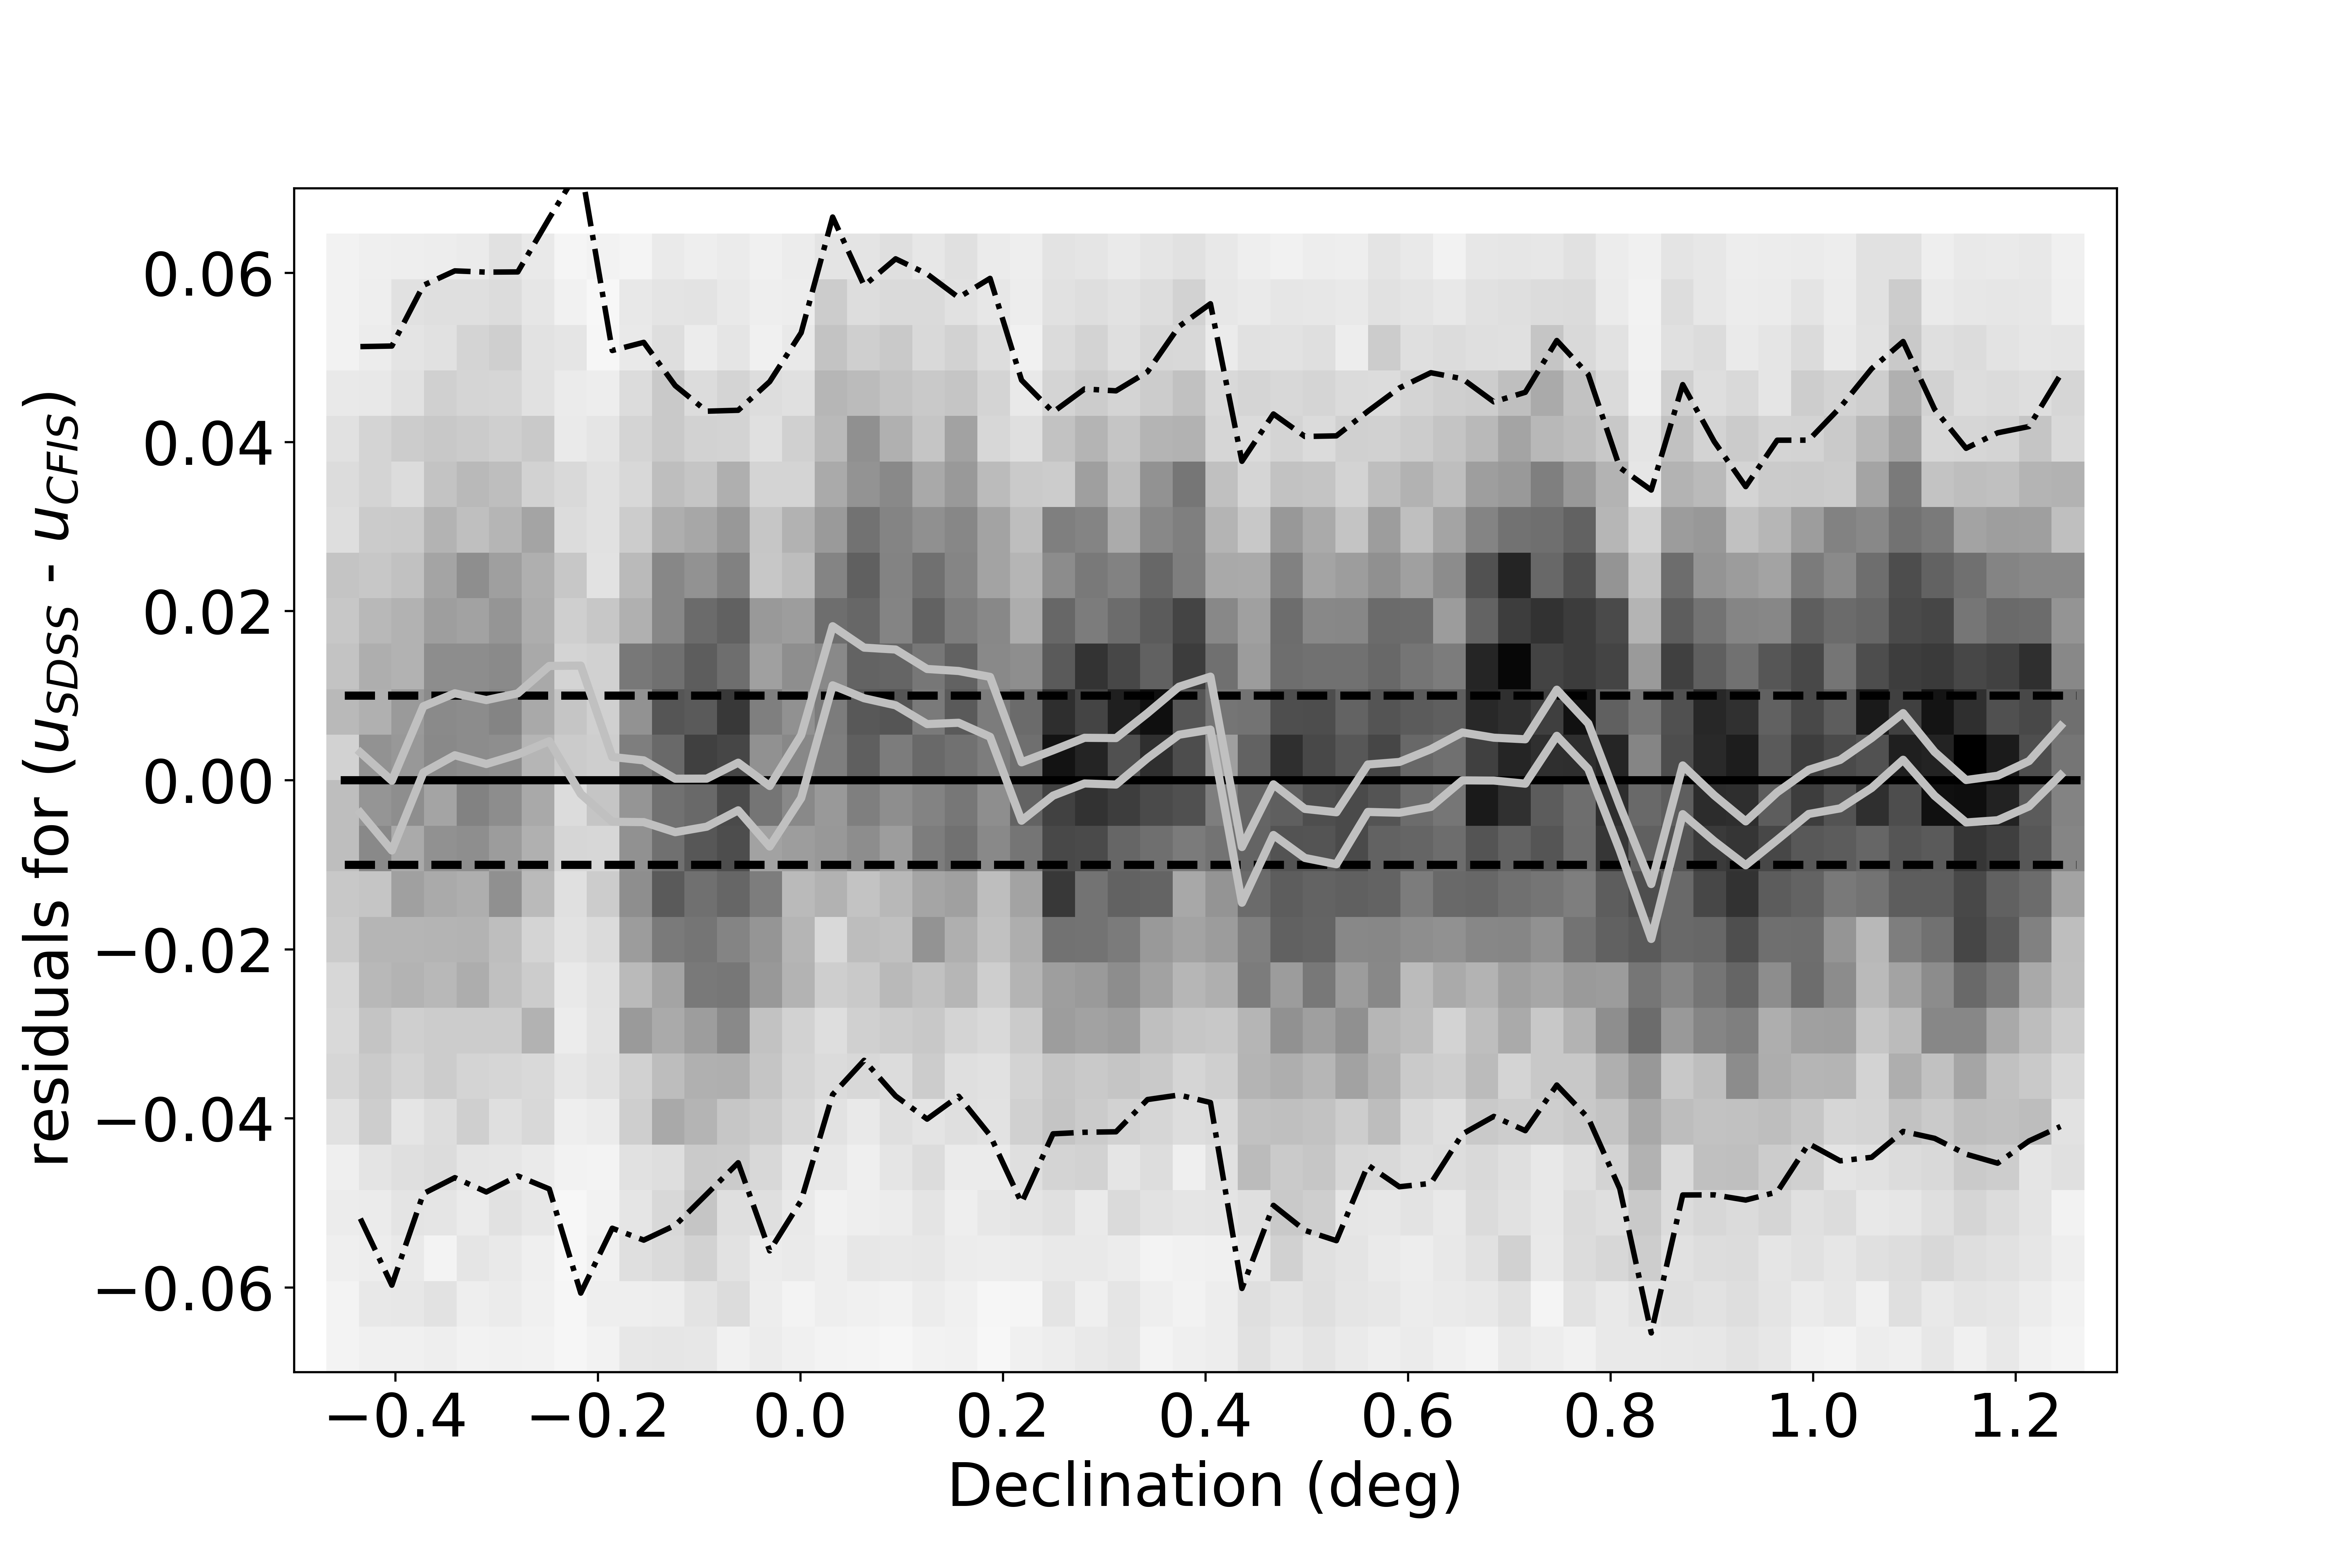
\includegraphics[width=9cm]{figures/colorResidCFISug_Dec_Hess.png} 
\caption{Analogous to Figure~\ref{fig:graycorrDec}, except that here residuals 
between the SDSS $u$ band magnitudes and $u$ band magnitudes from the CFIS
catalog (corrected for small color terms, $\sim0.05$ mag, as a function of the $u-g$ color),
for $\sim$150,000 matched stars with $1.0 <u-g < 2.1$ and $r<20$ are shown. 
The binned median scatter is 5.7 millimag. Note that the CFIS data are available
only for Declination $>$ -0.45 degree.}
\label{fig:CFIS}
\end{figure}

 